%% !TeX program = lualatex

%%%%%%%%%%%%%%%%%%%%%%%%%%%%%%%%%%%%%%%%%%%%%%%%%%%%%%%%%
% Niniejszy plik przedstawia przykładowy skład 
% pracy dyplomowej na Wydziale Matematyki PWr. 
% 
%
%%%%%%%%%%%%%%%%%%%%%%%%%%%%%%%%%%%%%%%%%%%%%%%%%%%%%%%%%
% Domyślną opcją jest: praca magisterska, język polski.
% W przypadku pracy pisanej w języku angielskim dodajemy 
% opcję [english]. 
% Dla pracy licencjackiej dodajemy opcję [licencjacka].
% Dla pracy inżynierskiej dodajemy opcję [inzynierska].
% Dopuszczalne są podwójne opcje, np. [licencjacka, english].
% Opcje dodajemy w kwadratowym nawiasie przy \documentclass.
%
%
%%%%%%%%%%%%%%%%%%%%%%%%%%%%%%%%%%%%%%%%%%%%%%%%%%%%%%%%%
\documentclass[english]{pwr_wmat_praca_dyplomowa}
%%%%%%%%%%%%%%%%%%%%%%%%%%%%%%%%%%%%%%%%%%%%%%%%%%%%%%%%%
%              DANE DO PRACY
%
% W przypadku pracy dyplomowej w języku angielskim nie jest konieczne 
% wypełnianie pól: \tytul{}, \kierunek{}, \specjalnosc{}, 
%                  \streszczenie{}, \slowakluczowe{}.
%%%%%%%%%%%%%%%%%%%%%%%%%%%%%%%%%%%%%%%%%%%%%%%%%%%%%%%%%
%
% Imię i nazwisko autora
\autor{Magdalena Wolniaczyk}
%
% Tytuł pracy dyplomowej 
% \tytul{Tytuł pracy dyplomowej} 
\tytulang{Comparison of Cognitive Diagnosis Models}
%
% Tytuł / stopień / imię i nazwisko opiekuna
\opiekun{Dr inż. Andrzej Giniewicz}
%
% Kierunek studiów wybieramy spośród następujących:
% 1) Matematyka
% 2) Matematyka i Statystyka
% 3) Matematyka stosowana
% \kierunekstudiow{Matematyka}
%
% Kierunek studiów po angielsku wybieramy spośród następujących:
% 1) Mathematics
% 2) Mathematics and Statistics
% 3) Applied Mathematics
\kierunekstudiowang{Applied Mathematics}
%
% Specjalność wybieramy spośród następujących: 
% KIERUNEK: Matematyka
% 1) Matematyka teoretyczna,
% 2) Statystyka matematyczna,
% 3) Matematyka finansowa i ubezpieczeniowa,
%
% KIERUNEK: Matematyka i Statystyka
% 4) Matematyka,
% 5) Statystyka i analiza danych, 
%
% 6) -- (w przypadku braku specjalizacji).
% \specjalnosc{Matematyka teoretyczna} 
%
% Specjalność w języku angielskim wybieramy spośród następujących:
% KIERUNEK: Matematyka
% 1) Theoretical Mathematics,
% 2) Mathematical Statistics,
% 3) Financial and Actuarial Mathematics,
%
% KIERUNEK: Matematyka i Statystyka
% 4) Mathematics,
% 5) Statistics and Data Analysis,
%
% KIERUNEK: Applied Mathematics
% 6) Financial and Actuarial Mathematics, 
% 7) Mathematics for Industry and Commerce,
% 8) Computational Mathematics,
% 9) Modelling, Simulation and Optimization.
%
% 10) -- (w przypadku braku specjalizacji).
\specjalnoscang{Data Engineering} 
%
% Krótkie streszczenia po polsku i angielsku
% - nie dłuższe niż 530 znaków.
% \streszczenie{Tutaj piszemy krótkie streszczenie pracy (nie powinno być dłuższe niż 530 znaków).}
\streszczenieang{Cognitive Diagnosis Models are one of the tools of mathematical cognitive psychology. Those models allow researchers to measure the skills of people based on some test results. The traits are described by latent variables. The test usually has dichotomous answers, which are linked to latent variables through a design matrix called the $Q$-matrix. The aim of this thesis was a comparison of commonly used models and measurement of their robustness. Furthermore, a~simulation study was conducted, to measure the effect of $Q$-matrix misspecification. Analysis of the real data set was attempted as well.}
%
% Podajemy najważniejsze słowa kluczowe po polsku i angielsku
% - w obu przypadkach, nie więcej niż 150 znaków.
% \slowakluczowe{tutaj podajemy najważniejsze słowa kluczowe (łącznie nie powinny być dłuższe niż 150 znaków).}  
\slowakluczoweang{Cognitive Diagnosis Models, $Q$-matrix, DINA, DINO, NIDA, G-NIDA, CDM validation, CDM robustness}
%
%
%%%%%%%%%%%%%%%%%%%%%%%%%%%%%%%%%%%%%%%%%%%%%%%%%%%%%%%%%
% Definicje, lematy, twierdzenia, przykłady i wnioski
% Komendy wywołujące twierdzenia, definicje, itd., 
% czyli 'theorem', 'definition', 'corollary', itd., 
% można zmienić wedle uznania.
\theoremstyle{plain}
\newtheorem{theorem}{Twierdzenie}
\numberwithin{theorem}{chapter}
\newtheorem{lemma}[theorem]{Lemma} 
\newtheorem{corollary}[theorem]{Wniosek}
\newtheorem{fact}[theorem]{Fact}
\theoremstyle{definition}
\numberwithin{theorem}{chapter}
\newtheorem{definition}[theorem]{Definition} 
\newtheorem{example}[theorem]{Example}
\newtheorem{note}[theorem]{Note}
%%%%%%%%%%%%%%%%%%%%%%%%%%%%%%%%%%%%%%%%%%%%%%%%%%%%%%%%%
\usepackage{tikz}
\usetikzlibrary{arrows}
\usepackage{tkz-graph}
\usepackage{multicol}
\usepackage{verbatim}
\usepackage{listings}

\usepackage{xcolor}

\definecolor{backcolour}{RGB}{251,251,251}
\definecolor{mygray}{RGB}{120,120,120}
\definecolor{myorange}{RGB}{226,77,54}
\definecolor{myblue}{RGB}{68,116,179}

\lstdefinestyle{codestyle}{
	backgroundcolor=\color{backcolour},   
	stringstyle=\color{myorange},
	keywordstyle=\color{myblue},
	numberstyle=\ttfamily\tiny\color{mygray},
	basicstyle=\ttfamily\footnotesize,
	breakatwhitespace=false,         
	breaklines=true,                 
	captionpos=b,                    
	keepspaces=true,                 
	numbers=left,                    
	numbersep=5pt,                  
	showspaces=false,                
	showstringspaces=false,
	showtabs=false,                  
	tabsize=3
}

\lstset{style=codestyle}

\usepackage{float}
\usepackage{booktabs}
%%%%%%%%%%%%%%%%%%%%%%%%%%%%%%%%%%%%%%%%%%%%%%%%%%%%%%%%%
%\makeatletter
%\patchcmd{\chapter}{\if@openright\cleardoublepage\else\clearpage\fi}{}{}{}
%\makeatother
%%%%%%%%%%%%%%%%%%%%%%%%%%%%%%%%%%%%%%%%%%%%%%%%%%%%%%%%%
\begin{document}
	\frontmatter
	\maketitle
	\mainmatter
	%\newpage\thispagestyle{empty}
	%\mbox{}
	%\newpage
	\tableofcontents
	%\listoffigures
	%\listoftables
	{\backmatter \chapter{Introduction}}
	
	Consider the case where teachers or researchers want to assess the abilities of the examinees. They need a tool that will allow them to clearly evaluate, not whether the students can solve an item correctly, but whether they have the skills that are needed to solve it. Cognitive Diagnosis Models are the tool that makes it possible. CDMs analysis can help to improve the quality of teaching and to provide feedback to students on their strengths and weaknesses because teachers will know how to enforce whether students have specific skills. They will be able to focus on those skills that are not mastered by students and help them to work on it.
	
	Cognitive Diagnosis Models are an area of psychometric research that has seen substantial growth in the past two decades, though the mathematics behind them, dating back to the year 1977. CDMs are latent class multidimensional statistical models that classify examinees as masters or non masters of different skills. CDMs can be categorized as either reduced or general (saturated) models. The reduced models are usually preferred due to the smaller number of parameters and their easy interpretation. However, they make strong assumptions about the data and model fit is therefore compromised. General models allow for greater flexibility, but with more demanding requirements. 
	
	In the real life, it is not known whether the obtained data can be modeled with a~specific model, so it is useful to know which model deals with the CDM misspecification and how a misspecified $Q$-matrix affects the obtained results. The purpose of this thesis is a~comparison of known Cognitive Diagnosis Models to find out the answer to this question. Moreover, the thesis is to show how the test and students' responses analysis with the use of CDMs looks like. 
	
	The first chapter contains a theoretical introduction to Cognitive Diagnosis Models, a detailed description of the models that will be analyzed and a description of methods in the field of mathematical statistics that will be used for estimation and its evaluation. The second chapter is devoted to simulations and their analysis. The first part concerns the CDM misspecification and is aimed at checking whether one of the analyzed models is more robust to mistake than the others. The models used in this section are DINA, DINO, NIDA and G-NIDA. The second part concerns a $Q$-matrix misspecification. Its~purpose is to check how the estimation is influenced by an incorrectly defined $Q$-matrix. Both parts contain relative and absolute fit evaluation and a summary of the obtained results. The third chapter is the analysis of the real data. The model which turned out to be the most robust was used for the estimation. This part of the work aims to show how Cognitive Diagnosis Models can be put into practice. On the basis of the obtained results, conclusions were drawn about the skills of students from the examined group. Then it was checked whether it is possible to improve the test that was used for the analysis by increasing and reducing the number of items in that test. The last part is a summary of the thesis and drawing conclusions.
	
	\chapter{Theory}
	
	\section{Cognitive Diagnosis Models}
	
	Traditional and most commonly employed models for measuring proficiency, like Item Response Theory (IRT) models or the Classical Test Theory (CTT) models (described in details in Weiner's book \cite{irt_ctt}), conceptualize examinee's knowledge as a~unidimensional latent construct. These types of models can be used for various purposes and they are the most useful in determining the position of one examinee relative to other examinees and the test items. Both IRT and CTT models provide single overall scores, but do not naturally provide sufficient diagnostic information \cite{de_la_torre_2016}. This need in educational assessments is met by the Cognitively Diagnostic Assessments (CDAs). CDAs are diagnostic tools, that is why statistical models which are capable of separating this level of information from the data are needed. Such models are called Cognitive Diagnosis Models (CDMs) or Diagnostic Classification Models (DCMs) \cite{de_la_torre_2014,dino_model}. 
	
	Cognitive Diagnosis Models offer an alternative psychometric framework for providing diagnostic information in the form of the examinee classification with respect to a set of attributes (skills). CDMs are latent class models that model responses as a function of discrete latent variables \cite{de_la_torre_2014}. 
	
	There are many examples of Cognitive Diagnosis Models in psychometric literature. Models can differ in different aspects, for example, it is possible to distinguish them by the possession of the skills for successfully mastering an item -- model can be compensatory (just one of the assigned skills has to be possessed) or non-compensatory (examinee has to possess all of the required skills). 
	
	In Table \ref{tab:cdms} on page \pageref{tab:cdms} few examples of Cognitive Diagnosis Models divided into compensatory and non-compensatory groups are presented. In Section \ref{section:cdm_misspec}, several of the models mentioned in the table, namely DINA, DINO, NIDA and G-NIDA, will be analyzed. 
	
	\begin{table}[t]
		\centering
		\small
		\begin{tabular}{l l c} 
			\hline  
			{\rule{0pt}{3ex}}Model & Model name & Model type \\ [0.5ex]
			\hline 
			{\rule{0pt}{3ex}}DINA & Deterministic Input Noisy ``And'' Gate Model \cite{dina_model} & \multirow{4}{*}{non-compensatory} \\
			NIDA & Noisy Input Deterministic Output ``And'' Gate Model \cite{nida_maris} \qquad & \\
			G-NIDA & Generalized NIDA Model \cite{nida_maris} & \\
			R-RUM & Reduced Reparameterized Unified Model \cite{rrum} & \\
			\hline
			{\rule{0pt}{3ex}}DINO & Deterministic Input Noisy ``Or'' Gate Model \cite{dino_model} & \multirow{4}{*}{compensatory}\\
			NIDO & Noisy Input Deterministic Output ``Or'' Gate Model \cite{book_models} & \\
			A-CDM & Additive Cognitive Diagnosis Model \cite{de_la_torre_2011} & \\
			C-RUM & Compensatory Reparameterized Unified Model \cite{rrum} & \\ [0.5ex] 
			\hline
		\end{tabular}
		\caption{Examples of Cognitive Diagnosis Models.}
		\label{tab:cdms} 
	\end{table}
	
	\subsection{Input and output in a CDMs analysis}
	
	The analysis and estimation of Cognitive Diagnosis Models require two input matrices. The first matrix contains the item responses of examinees and it is called the response matrix. The second one is called $Q$-matrix and it specifies the relationship between each item on a~test and content-related skills \cite{gdina_in_r}. The details and definitions concerning inputs in CDMs analysis are going to be explained in Section \ref{section:term_notation}. 
	
	\newpage
	The aim of conducting a Cognitive Diagnosis Models analysis is to be able to draw conclusions about examinees’ possession of the specific, defined skills. The expression ``examinees’ possession of the skills'' includes answers for many different questions. Thanks to the analysis of CDMs it is possible, for example, to get to know the population skill possession -- the percentage of examinees from the study group who possess each skill, the population skill class distribution -- the percentage of examinees who possess specific skills combination called skill profile (precise explanation of this phrase is provided in Section \ref{section:term_notation}) or the individual skill possession -- individual skill profiles of the examinees \cite{cdm_in_r}. Such an analysis will be conducted and the results are going to be interpreted in Chapter \ref{chapter:real_data}.
	
	\section{Terminology and notation}\label{section:term_notation}
	
	Before analyzing the structure of specific Cognitive Diagnosis Models it is necessary to become familiar with several important terms which were mentioned in the previous section: the response matrix, the $Q$-matrix, and the skill profile.
	
	\subsection{Response matrix}
	
	Consider the test in which \textit{I} examinees respond to \textit{J} items. A value of $1$ indicates a~correct response to the item and a value of $0$ an incorrect one. This is exactly so-called item response data, which is stored in a $I \times J$ binary data matrix $X$ called response matrix.
	
	The~dichotomous response of student \textit{i}, $i = 1, \ldots , I$, to item \textit{j}, $j = 1, \ldots , J$, is expressed by $x_{ij} \in \{0,1\}$. The $j$-th column of the matrix $X$ represents the responses of all $I$ examinees to $j$-th item and the $i$-th row of the matrix $X$ indicates the responses of examinee $i$ to all $J$~items (it is called response pattern). In Table \ref{tab:responsemat} on page \pageref{tab:responsemat} the example of the response matrix is presented.
	
	\begin{table}[t]
		\centering
		\begin{tabular}{c c c c c c} 
			\hline
			{\rule{0pt}{3ex}} & \multicolumn{5}{c}{Item} \\
			Examinee & 1 & 2 & 3 & \ldots & J \\ [0.5ex] 
			\hline
			1 & 1 & 1 & 0 & & 1 \\ 
			2 & 0 & 0 & 1 & & 0 \\
			3 & 1 & 0 & 1 & & 1 \\
			4 & 1 & 0 & 1 & & 0 \\
			\vdots & & & & & \\
			I & 1 & 1 & 0 & & 1\\ [1ex] 
			\hline
		\end{tabular}
		\caption{The example of the response matrix $X_{I \times J}$.}
		%\caption*{\textit{Źródło: opracowanie własne}}
		\label{tab:responsemat} 
	\end{table}
	
	\subsection{Q-matrix}
	
	The binary $J \times K$ weight matrix (called $Q$-matrix) reflects which skills (also called attributes) are measured by each item. In $Q$-matrix $(j,k)$-th element $q_{jk}$, $(j=1,\ldots,J, \: k=1,\ldots,K)$, expresses whether skill $k$ is relevant for the mastery of item $j$ $(q_{jk} = 1)$ or if skill is not needed for correctly responding to item $(q_{jk} = 0)$ \cite{cdm_in_r}. 
	
	Creating $Q$-matrix is not an easy procedure and it should have a solid theoretical foundation. The $Q$-matrix construction process involves the qualitative work of experts after a literature review and analyzing domain specialists' reports. First, the experts subdivide the tested overall domain into a few skills according to a~well-established relationship between the skills (labelled by $\alpha_k, \: k = 1,\ldots,K$). Secondly, based on the~relationship between the skills, the experts specify which attributes $\alpha_k$ are required for giving a~positive response in each test item. Thus, the weight matrix $Q$ reflects the essential theory of how attributes contribute to answering each item. This process is subjective and can lead to some misspecifications in the $Q$-matrix, which negatively affect the accuracy of the skill profile classification \cite{de_la_torre_2016}. This problem will be considered in Section \ref{section:qmat_misspec}. In Table \ref{tab:qmatrix} the example of the $Q$-matrix is presented.
	
	\begin{table}[H]
		\centering
		\begin{tabular}{c c c c c c} 
			\hline
			{\rule{0pt}{3ex}} & \multicolumn{5}{c}{Skill} \\
			Item & $\alpha_1$ & $\alpha_2$ & $\alpha_3$ & \ldots & $\alpha_K$ \\ [0.5ex] 
			\hline
			1 & 1 & 1 & 0 & & 1 \\ 
			2 & 0 & 1 & 0 & & 0 \\
			3 & 1 & 0 & 1 & & 1 \\
			4 & 0 & 0 & 1 & & 0 \\
			\vdots & & & & & \\
			J & 0 & 0 & 1 & & 1\\ [1ex] 
			\hline
		\end{tabular}
		\caption{The example of the weight matrix $Q_{J \times K}$.}
		\label{tab:qmatrix} 
	\end{table}
	
	\subsection{Skill profile}\label{subsec:skill_prof}
	
	After defining $Q$-matrix, it is already known which skills are necessary to master each item. The examinee has to possess  $K$ $(K\leq J)$ skills $\alpha_k$ ($k=1,\ldots,K$) to correctly answer each of the $J$ items. 
	
	For each examinee $i$ a skill profile (called also knowledge state) $\alpha_i = (\alpha_{i,1}, \alpha_{i,2}, \ldots, \alpha_{i,K})$ denotes his actual possession of the $K$ predefined attributes (construed as a binary event). If examinee possesses a~particular skill $\alpha_{ik}=1$, otherwise $\alpha_{ik}=0$. For $K$ attributes a~set of all possible skill combinations contains $2^K$ skill classes. Thus each examinee profile belongs to one of the~skill classes. 
	
	Obviously, during the analysis of pieces of information contained in the response data, individual skill profiles of examinees are unknown. One of the goals of the CDMs analysis is to estimate them and and draw conclusions regarding a single examinee or the entire group of respondents. Table \ref{tab:skillprofile} on page \pageref{tab:skillprofile} shows all possible skill combinations for the three analyzed skills $K=3$. The examinee solving the test that studies three skills may have a skill profile corresponding to one of the rows in this table.
	
	\begin{table}[H]
		\centering
		\begin{tabular}{c c c c} 
			\hline
			{\rule{0pt}{3ex}} & \multicolumn{3}{c}{Skill} \\
			Profile & $\alpha_1$ & $\alpha_2$ & $\alpha_3$ \\ [0.5ex] 
			\hline
			1 & 0 & 0 & 0 \\ 
			2 & 0 & 0 & 1 \\
			3 & 0 & 1 & 0 \\
			4 & 1 & 0 & 0 \\
			5 & 0 & 1 & 1 \\
			6 & 1 & 0 & 1 \\ 
			7 & 1 & 1 & 0 \\
			8 & 1 & 1 & 1\\[1ex] 
			\hline
		\end{tabular}
		\caption{All possible skills combinations for $K=3$ ($2^K = 2^3 = 8$).}
		\label{tab:skillprofile} 
	\end{table}
	
	\section{The DINA model}
	
	The DINA model -- the deterministic input, noisy, ``and'' gate model is one of the most commonly used Cognitive Diagnosis Models (mostly because of its simplicity). It was precisely examined in 1989 by Haertel who identified it as a restricted latent class model~\cite{dina_model}. 
	
	The DINA model possesses an important and restrictive property. This model is non-compensatory -- there is no possibility of compensating for a lack of one skill by having an excess of another. The ``and gate'' component of the model name refers to that -- a~correct response to an~item is possible only when the examinee possesses all the prescribed skills for successfully mastering it (a conjunctive condensation rule). Only possessing all of the required attributes to solve respective item, increases the probability of a positive response to an item. 
	
	The \textit{i}-th examinee's probability to master the \textit{j}-th item involves two components: a~deterministic and a~probabilistic one, which correspond to the property mentioned before. 
	
	The deterministic component is expected examinee's \textit{i} response to the item \textit{j} expressed through dichotomous latent response variable defined as
	\begin{equation}
	\eta_{ij} = \prod\limits_{k=1}^{K} \alpha_{ik}^{q_{jk}} \in \{0,1\},
	\end{equation}
	
	\noindent where $q_{jk}$ denotes the element of the $Q$-matrix, which expresses whether skill \textit{k} is needed or~not to positively respond to an item \textit{j} and latent vector $\alpha_{ik}$ is skill profile. Deterministic latent response $\eta_{ij}$ (prediction of an item performance from examinee's knowledge state) is called also ideal response pattern. % (terminology by Tatsouka 1995). 
	
	The examinee \textit{i} who possesses at least all of the skills required for the mastery of an~item \textit{j} is expected to respond to item positively ($\eta_{ij} = 1$). Otherwise, if the examinee lacks at least one of the required skills, he is not expected to respond to item positively ($\eta_{ij} = 0$). When the examinee do not possess skill ($\alpha_{ik} = 0$) and the skill is not needed to positively respond to an item ($q_{jk} = 0$), then the value $\alpha_{ik}^{q_{jk}} = 0^0$ in the expected examinee's \textit{i} response to the item \textit{j} ($\eta_{ij}$) is treated as 1.
	
	The second component, probabilistic, includes possibilities that even if the examinee is expected to master the item, he nevertheless may slip and fail to produce a positive response (false positive error) or on the other hand, even if the examinee is not expected to positively respond the item, he may succeed by a lucky guess of the correct response (false negative error). Those two possibilities are called probabilistic error components. The~slipping parameter $s_j$ is the probability that the first event appears although the probability that the second event occurs is the guessing parameter $g_j$ \cite{de_la_torre_2011}. Formally, the~probabilistic error components are defined as: 
	\begin{equation}
	s_j = P(X_{ij} = 0 | \eta_{ij} = 1),
	\end{equation}
	\begin{equation}
	g_j = P(X_{ij} = 1 | \eta_{ij} = 0).
	\end{equation}
	
	When the chances of slipping $s_j$ and guessing $g_j$ have been determined and when the deterministic latent response $\eta_{ij}$ is known, the probability of the \textit{i}-th examinee to solve item \textit{j} -- the correct response probability in~the~DINA model -- can be computed. It~results from combining the expected response and the probabilistic error components and for a~single item it is expressed by
	\begin{equation}
	P(X_{ij} = 1 | \alpha_i, g_j, s_j) = (1-s_j)^{\eta_{ij}} \cdot g_j^{(1-\eta_{ij})} = \left\{ \begin{array}{ll}
	1 - s_j & \textrm{for $\eta_{ij} = 1$,} \\
	g_j & \textrm{for $\eta_{ij} = 0$.} 
	\end{array}\right.
	\end{equation}
	
	The DINA model involves only two probabilities for responding to the item \textit{j}: the~examinee who is not expected to master the item have the chance $g_j$ to solve the item by luckily guessing the solution, and the examinee who is expected to master the item have the chance $1 - s_j$ to give the correct answer to the item without slipping. There is no difference if the examinee has only one of the required skills missing or if he does not possess any of them -- slipping and guessing probabilities will have the same value and the correct response probability will not change. Table \ref{tab:response_prob} contains all possible correct response probabilities in the DINA model.
	
	\begin{table}[H]
		\centering
		\begin{tabular}{l c c} 
			\hline
			{\rule{0pt}{3ex}} & $X_{ij} = 1$ & $X_{ij} = 0$ \\
			& (correct response) & (incorrect response) \\ [0.5ex]
			\hline 
			{\rule{0pt}{3ex}} $\eta_{ij} = 1$ & $1- s_j$ & $s_j$ \\ 
			(mastery of all measured attributes) & & \\[1ex] 
			$\eta_{ij} = 0$ & $g_j$ & $1-g_j$ \\ 
			(lack of at least one measured attribute) & & \\[0.5ex] 
			\hline
		\end{tabular}
		\caption{Response probabilities in the DINA model \cite{book_tables}.}
		\label{tab:response_prob} 
	\end{table}
	
	In Figure \ref{graph_dina} on page \pageref{graph_dina}, there is a scheme showing the $i$-th examinee response process to item $j$ in~the~DINA model. At the top of the scheme are placed: examinee's skill profile ($A$) and $q$-vector ($Q$), which is a $Q$-matrix row and gives information about the skills required for the item $j$. Both $A$ and $Q$ are essential elements to know deterministic latent responses of the examinee $N$. Those responses can take the values 0 or 1 as shown in Figure \ref{graph_dina}. Taking the value 0 or 1 results in the fact that the correct response ($X=1$) probability depends on the guessing parameter ($G$) or the slipping parameter ($S$), respectively.
	
	\begin{figure}[h!]
		\centering
		\begin{multicols}{2}
			\begin{tikzpicture}
			\GraphInit[vstyle=Empty]
			\Vertex{$A$}
			\Vertex[x=4,y=0]{$Q$}
			\Vertex[x=2,y=-1.5]{$N$}
			\Vertex[x=0,y=-3]{0}
			\Vertex[x=4,y=-3]{1}
			\Vertex[x=0,y=-4.5]{$G$}
			\Vertex[x=4,y=-4.5]{$S$}
			\Vertex[x=2,y=-6]{$X=1$}
			\Edges($A$,$N$,$Q$) 
			\Edges(0,$N$,1)
			\Edges(0,$G$)
			\Edges(1,$S$)
			\Edges($G$,$X=1$,$S$)
			\end{tikzpicture}
			
			Where symbols on a graph mean:
			\begin{itemize}
				\item $A = (\alpha_{i1}, \alpha_{i2}, \ldots, \alpha_{iK} )^{'}$
				\item $Q = (q_{j1}, q_{j2}, \ldots, q_{jK} )^{'}$
				\item $N = \eta_{ij} = \prod\limits_{k=1}^{K} \alpha_{ik}^{q_{jk}}$
				\item $G = g_j$
				\item $S = 1-s_j$
				\item $X = X_{ij}$
				\item $P(X_{ij} = 1 | \eta_{ij}) = (1-s_j)^{\eta_{ij}} \cdot g_j^{1-\eta_{ij}}$
			\end{itemize}
		\end{multicols} 
		\caption{A graphical representation of the $i$-th examinee response process to item $j$ in~the~DINA model \cite{de_la_torre_2009}.}\label{graph_dina}
	\end{figure}
	
	\section{The DINO model}
	
	The DINO model -- the deterministic input, noisy, ``or'' gate model is next to the DINA model one of the most popular Cognitive Diagnosis Models. It was considered in detail by Templin and Henson in 2006 \cite{dino_model}. On the contrary to the DINA model, the DINO model is compensatory, what means that the model requires the examinee to possess at least one of the prescribed skills for successfully mastering the respective item (a disjunctive condensation rule) and ``or gate'' component of the model name refers to that. 
	
	Same as previously, the \textit{i}-th examinee's probability to master the \textit{j}-th item involves two components: a~deterministic and a~probabilistic one. 
	
	In the DINO model, expected examinee's \textit{i} response to the item \textit{j} expressed through the deterministic latent response defined as
	\begin{equation}
	\eta_{ij} = 1- \prod\limits_{k=1}^{K} \left( 1 - \alpha_{ik} \right)^{q_{jk}} \in \{0,1\},
	\end{equation}
	where $q_{jk}$ denotes the element of the $Q$-matrix, which expresses whether skill \textit{k} is needed or not to positively respond to an item \textit{j} and latent vector $\alpha_{ik}$ is a skill profile.
	
	The examinee \textit{i} who possesses at least one of the skills required for the mastery of an~item \textit{j} is expected to respond to item positively ($\eta_{ij} = 1$). Otherwise, if the examinee does not possess any of the required skills, he is not expected to respond to the item positively ($\eta_{ij} = 0$). In the case when the examinne possesses skill, which is not needed, the value $\left(1 - \alpha_{ik} \right)^{q_{jk}} = 0^0$ is treated as 1.
	
	Remaining part of the DINO model looks the same as in the DINA model. The~probabilistic error components are $s_j$ for slipping in item \textit{j} and $g_j$ for guessing item \textit{j}:
	\begin{equation}
	s_j = P(X_{ij} = 0 | \eta_{ij} = 1),
	\end{equation}
	\begin{equation}
	g_j = P(X_{ij} = 1 | \eta_{ij} = 0).
	\end{equation}
	
	\noindent The probability of the \textit{i}-th examinee to solve item \textit{j} is expressed through
	\begin{equation}
	P(X_{ij} = 1 | \alpha_i, g_j, s_j) = (1-s_j)^{\eta_{ij}} \cdot g_j^{(1-\eta_{ij})} = \left\{ \begin{array}{ll}
	1 - s_j & \textrm{for $\eta_{ij} = 1$,} \\
	g_j & \textrm{for $\eta_{ij} = 0$.} 
	\end{array}\right.
	\end{equation}
	
	Again probability for a correct response to an item is modelled by only two values: the examinee who is expected to master the item have the chance $1 - s_j$ for solving it without slipping and the examinee who is not expected to master the item have the chance $g_j$ for solving it by a lucky guess. All possible correct response probabilities in the DINO model are presented in Table \ref{tab:response_prob2}.
	
	\begin{table}[H]
		\centering
		\begin{tabular}{l c c} 
			\hline
			{\rule{0pt}{3ex}} & $X_{ij} = 1$ & $X_{ij} = 0$ \\
			& (correct response) & (incorrect response) \\ [0.5ex]
			\hline 
			{\rule{0pt}{3ex}} $\eta_{ij} = 1$ & $1- s_j$ & $s_j$ \\ 
			(presence of at least one measured attribute) & & \\[1ex] 
			$\eta_{ij} = 0$ & $g_j$ & $1-g_j$ \\ 
			(lack of all measured attributes) & & \\[0.5ex] 
			\hline
		\end{tabular}
		\caption{Response probabilities in the DINO model \cite{book_tables}.}
		\label{tab:response_prob2} 
	\end{table}
	
	Due to the high similarity of the DINO model to the DINA model, it is also possible to present a scheme of the $i$-th examinee response process to item $j$ (Figure \ref{graph_dino}). Again, at the top of the scheme are placed: examinee's skill profile ($A$) and $q$-vector ($Q$). Both $A$ and $Q$ are essential elements to know deterministic latent responses of the examinee $N$, whose definition differs from those shown in Figure \ref{graph_dina}. Deterministic latent responses can take the values 0 or 1 and it results in the fact that the correct response ($X=1$) probability depends on the guessing parameter ($G$) or the slipping parameter ($S$), respectively.
	
	\begin{figure}[!ht]
		\centering
		\begin{multicols}{2}
			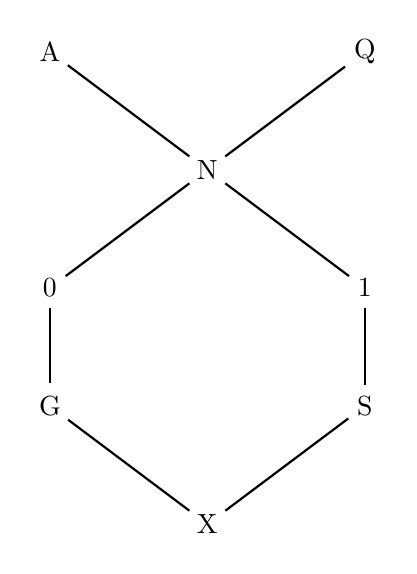
\begin{tikzpicture}
			\GraphInit[vstyle=Empty]
			\Vertex{A}
			\Vertex[x=4,y=0]{Q}
			\Vertex[x=2,y=-1.5]{N}
			\Vertex[x=0,y=-3]{0}
			\Vertex[x=4,y=-3]{1}
			\Vertex[x=0,y=-4.5]{G}
			\Vertex[x=4,y=-4.5]{S}
			\Vertex[x=2,y=-6]{X}
			\Edges(A,N,Q) 
			\Edges(0,N,1)
			\Edges(0,G)
			\Edges(1,S)
			\Edges(G,X,S)
			\end{tikzpicture}
			
			Where symbols on a graph mean:
			\begin{itemize}
				\item $A = (\alpha_{i1}, \alpha_{i2}, \ldots, \alpha_{iK} )^{'}$
				\item $Q = (q_{j1}, q_{j2}, \ldots, q_{jK} )^{'}$
				\item $N = \eta_{ij} = 1- \prod\limits_{k=1}^{K} \left( 1 - \alpha_{ik} \right)^{q_{jk}}$
				\item $G = g_j$
				\item $S = 1-s_j$
				\item $X = X_{ij}$
				\item $P(X_{ij} = 1 | \eta_{ij}) = (1-s_j)^{\eta_{ij}} \cdot g_j^{1-\eta_{ij}}$
			\end{itemize}
		\end{multicols} 
		\caption{A graphical representation of the \textit{i}-th examinee response process to item \textit{j} in~the~DINO model \cite{de_la_torre_2009}.}\label{graph_dino}
	\end{figure}
	
	\section{The NIDA model}
	
	The noisy inputs, deterministic, ``and'' gate model (NIDA) was discussed in 1999 by Maris \cite{nida_maris} and described in detail by Junker and Sijtsma in 2001 \cite{nida_model}. Like DINA, the NIDA model belongs to the non-compensatory type of models, and the same as the DINA model it is an example of models with a conjunctive condensation rule (all required attributes need to be present). The difference between those two models is that in the DINA model there is no matter which skill or skills are missing -- probability for a correct response to an item is the same, NIDA model distinguishes these cases and probability differs depending on missing attributes. 
	
	For the NIDA model, variables $X_{ij}$, $\alpha_{ik}$, and $q_{jk}$ which were described earlier and the latent variable $\zeta_{ijk}$ are needed. Variable $\zeta_{ijk} \in \{0,1\}$ indicates whether examinee $i$ correctly apply an attribute $k$ for the item $j$ (examinee's performance in the context of an~item is compatible with possessing skill $\zeta_{ijk}=1$ or noncompatible $\zeta_{ijk}=0$) \cite{book_tables}. The examinee's response, in turn, is~related to the definition of slipping and guessing parameters.
	
	Already described DINA and DINO models both model slipping and guessing processes at the item level. In the NIDA model, in contrast to DINA and DINO, guessing and slipping occur at the skill rather than item level. To summarize, the latent variables $\zeta_{ijk}$ are related to the examinee's skill profiles $\alpha_{i}$ according to the probabilities
	
	\begin{equation}
	s_k = P(\zeta_{ijk} = 0 | \alpha_{ik} = 1, q_{jk} = 1),
	\end{equation}
	\begin{equation}
	g_k = P(\zeta_{ijk} = 1 | \alpha_{ik} = 0, q_{jk} = 1),
	\end{equation}
	and, what is important,
	\begin{equation}
	P(\zeta_{ijk} = 1 | q_{jk} = 0) \equiv 1,
	\end{equation}
	no matter what is the value of $\alpha_{ik}$ (can take any value $\alpha \in \{0,1\}$). The observed response to the item $j$ by examinee $i$ is expressed through
	\begin{equation}
	X_{ij} = \prod\limits_{k=1}^{K} \zeta_{ijk}.
	\end{equation}
	
	\noindent While the slipping $s_k$ and guessing $g_k$ parameters (probabilities of correctly applying each of the measured skills) are determined and while the skill profile $\alpha_{i}$ and the weight matrix $Q_{J\times K}$ are known, the correct response probability in~the~NIDA model (the probability of correctly applying measured skills for the item) can be computed. The correct response probability for a single item is expressed through 
	\begin{equation}
	P(X_{ij} = 1 | \alpha_i, g, s) = \prod\limits_{k=1}^{K} P(\zeta_{ijk} = 1 | \alpha_{ik}, q_{jk}) = \prod\limits_{k=1}^{K} \left[ (1-s_k)^{\alpha_{ik}} \cdot g_k^{(1-\alpha_{ik})} \right] ^{q_{jk}}.
	\end{equation}
	
	The NIDA model has restrictive assumptions -- constraints of equality across the items. This means that the model provides one slipping ($s_k$) and one guessing ($g_k$) parameter per skill, but the values of slipping and guessing parameters have to be the same across the items. The number of model parameters is not influenced by the number of items, it~increases with the number of skills. 
	
	An extension of the NIDA model is the generalized noisy inputs, deterministic, ``and''~gate (G-NIDA) model where the slipping and guessing parameters are permitted to differ also across the items. 
	
	\section{The G-NIDA model}
	
	The generalized noisy inputs, deterministic, ``and'' gate (G-NIDA) model is an extension of the NIDA model. In the G-NIDA model slipping and guessing parameters are allowed to vary not only across the attributes but also across the items
	\begin{equation}
	s_{jk} = P(\zeta_{ijk} = 0 | \alpha_{ik} = 1, q_{jk} = 1),
	\end{equation}
	\begin{equation}
	g_{jk} = P(\zeta_{ijk} = 1 | \alpha_{ik} = 0, q_{jk} = 1).
	\end{equation}
	
	\noindent This property leads to the correct response probability in the G-NIDA model in the form
	\begin{equation}
	P(X_{ij} = 1 | \alpha_i, g_j, s_j) = \prod\limits_{k=1}^{K} \left[ (1-s_{jk})^{\alpha_{ik}} \cdot g_{jk}^{(1-\alpha_{ik})} \right] ^{q_{jk}},
	\end{equation}
	where the terms above are the same as described in the description of the NIDA model.
	
	\section{Methodology}
	
	In this Section the procedure and the methods used to carry out the simulations and test their quality are described: the Joint Maximum Likelihood Estimation, which was used for fitting Cognitive Diagnosis Models (CDMs), and the statistics and measures necessary to evaluate these fits: log-likelihood value, Akaike and Bayesian Information Criteria and measures based on confusion matrix (accuracy, informedness, markedness, and their geometric mean).
	
	\subsection{Joint Maximum Likelihood Estimation}
	
	The Joint maximum likelihood estimation (JMLE) is a parameteric approach to fit a~Cognitive Diagnosis Models to the response data an estimate both the item parameters and examinee attribute profiles\footnote{Source: https://cran.r-project.org/web/packages/NPCD/NPCD.pdf (access: VIII 2020)}. Joint Maximum Likelihood Estimation procedure involves maximizing the overall likelihood function by means of the parameter estimates obtained by the separate MLE procedures for the items and examinees. The intent is to obtain a~global maximum for the overall likelihood function. 
	
	As is known from Section \ref{section:term_notation}, $I$ examinees possess their skill profiles and each of these examinees responds to the $J$ items of the test. The responses are dichotomously scored, $x_{ij} \in \{0,1\}$, where $i$ $(i = 1, 2, \ldots, I)$ indicates the examinee and $j$ $( j = 1, 2, \ldots, J)$ defines the item. 
	For each examinee there is a vector of item responses of length $J$ denoted by $(x_{i1}, x_{i2}, \ldots, x_{iJ} | \theta_i)$, where $\theta_i$ is $K$-dimensional latent vector (the examinee's skill profile). Under the local independence assumption (a standard assumption for item factor analysis), the $x_{ij}$ are statistically independent for all examinees having the same skill profile. The~resulting $I \times J$ matrix of item responses (the response matrix) is already known as $X$. If~$\Theta$ is the vector of all examinees' skill profiles $(\theta_1, \theta_1, \ldots, \theta_I)$, the probability of $X$ is given by the joint likelihood function specified \cite{jmle} as
	
	\begin{equation}
	\mathcal{L}(\Theta|X) = P(X|\Theta) = \prod_{i=1}^{I} \prod_{j=1}^{J} \text{P}_j (\theta_i)^{x_{ij}} \text{Q}_j(\theta_i)^{1-x_{ij}},
	\end{equation}
	
	\noindent where $\text{P}_j (\theta_i) = P(x_{ij}=1|\theta_i) $ is a probability of the $i$-th examinee correct response to the $j$-th item and $\text{Q}_j = 1 - \text{P}_j$. As typically, it is the natural logarithm of the likelihood function that one maximizes. So, the function being maximized is given by
	% https://link.springer.com/chapter/10.1007/978-3-319-77249-3_28
	\begin{equation}
	l(\Theta|X) = \log\: \mathcal{L}(\Theta|X) = \sum_{i=1}^{I} \sum_{j=1}^{J} \left[ x_{ij}\; \log\: \text{P}_j(\theta_i) + (1-x_{ij})\; \log\:  \text{Q}_j(\theta_i) \right].
	\end{equation}
	
	\noindent Thus, the Joint Maximum Likelihood Estimator is defined \cite{jmle2} as
	
	\begin{equation}
	\hat{\Theta} = \underset{\Theta}{\arg\max} \: l(\Theta|X). 
	\end{equation}
	
	\texttt{JMLE()} function in \texttt{NPCD} library returns Joint Maximum Likelihood Estimates of item parameters and examinee skill profile in CDMs. The algorithm starts from the nonparametric estimation of skill profiles for both the conjunctive and disjunctive CDMs, implemented by the \texttt{AlphaNP()} function. Algorithms choose the skill profile with the smallest loss function value. When the attribute profiles are chosen, then the \texttt{JMLE()} function iteratively estimates item parameters and skill profiles using MLE until the algorithm converges\footnote{Source: https://cran.r-project.org/web/packages/NPCD/NPCD.pdf (access: VIII 2020)}.
	
	\subsection{Log-likelihood value}
	
	Log-likelihood value is a measure of goodness of fit for any model. Log-likelihood can take values between $-\infty$ to $+\infty$. Higher the value of log-likelihood, better is the fit of the model. Log-likelihood value belongs to relative fit evaluation type because it is a~function of sample size, which means that it cannot be used alone as an index of fit and the absolute look at the value cannot give any indication but it can be used to compare the fit between different models \cite{statistics}. %\footnote{Source: https://medium.com/@analyttica/log-likelihood-analyttica-function-series-cb059e0d379 (access: VIII 2020)}. 
	
	\subsection{AIC and BIC criteria}
	
	Akaike and Bayesian information criteria are the two most commonly used criteria in model
	selection and they are both penalized-likelihood criteria. They are goodness-of-fit tests to assess the
	performance of a model with respect to how well it explains the data. AIC and BIC also belong to relative fit evaluation, thus they can only be used for comparison of the fit between different models. A lower AIC or BIC value indicates a better fit \cite{aic_bic}.
	
	\subsubsection{Akaike information criterion}
	
	Akaike information criterion was proposed by Akaike in 1974 \cite{aic}. The formula for AIC is as follows
	
	\begin{equation}
	AIC = -2 \log{\mathcal{L}(\hat{\Theta})} + 2k,
	\end{equation}
	
	\noindent where $\Theta$ is the vector of model parameters, $\mathcal{L}(\hat{\Theta})$ is the value of the likelihood function and $k$ is the number of estimated parameters. 
	
	The first element is the value of the likelihood function, which is the probability of obtaining the data given the candidate model, multiplied by $-2$. Ignoring the second element, the model with the~minimum AIC is the best one. However, to the first component is added the number of estimated parameters multiplied by 2. The more parameters, the higher the value of the AIC, which means that the model is penalized for its complexity. As a~result, it has to be considered whether a better fit by creating a more complex model is worth the penalty imposed by requiring more parameters.
	
	\subsubsection{Bayesian information criterion}
	
	Bayesian information criterion was proposed by Schwarz in 1978 \cite{bic}. It is another model selection criterion based on information theory and it is closely related to the Akaike information criterion. The formula for BIC is as follows
	
	\begin{equation}
	BIC = -2 \log{\mathcal{L}(\hat{\Theta})} + k\log{n},
	\end{equation}
	
	\noindent where $\Theta$ is the vector of model parameters, $\mathcal{L}(\hat{\Theta})$ is the value of the likelihood, $k$ is the number of estimated parameters and $n$ is the number of observations (sample size). 
	
	The difference between the AIC and the BIC is the penalty imposed for the number of parameters, it is larger in BIC than in AIC. The penalty in BIC resolves the problem of overfitting, which is possible in AIC because of increasing the likelihood by adding parameters.
	
	\subsection{Confusion matrix}
	
	The confusion matrix is an $N \times N$ matrix, where columns correspond to the correct decision classes and rows correspond to decisions predicted by the classifier. The number $n_{ij}$ at the intersection of row $i$ and column $j$ is the number of examples from the $j$-th class that were classified to the $i$-th class. A more general name for a confusion matrix is contingency table. Special attention is given to $2 \times 2$ tables, where all possible results in the binary classification are:
	
	\begin{itemize}
		\item True Positive -- the observation was positive and was classified as positive,
		\item False Positive -- the observation was negative and was classified as positive,
		\item False Negative -- the observation was positive and was classified as negative,
		\item True Negative -- the observation was negative and was classified as negative,
	\end{itemize}
	
	\noindent and they are presented in Table \ref{tab:confusion_matrix}.
	
	\begin{table}[H]
		\centering
		\begin{tabular}{c c | c | c} 
			& & \multicolumn{2}{c}{Actual class} \\
			& & Positive & Negative \\
			\hline
			{\rule{0pt}{3ex}} \multirow{2}{*}{Predicted class} & Positive & True Positive (TP) & False Positive (FP) \\\cmidrule{2-4}
			& Negative & False Negative (FN) & True Negative (TN)  \\
		\end{tabular}
		\caption{The confusion matrix.}
		\label{tab:confusion_matrix} 
	\end{table}
	
	The definitions of all measures come from the work of D. Powers \cite{powers2011evaluation}, but before defining mentioned earlier accuracy, informedness and markedness, it is worth to know the basic measures:
	
	\begin{itemize}
		\item Sensitivity (also called Recall or True Positive Rate) is the ratio of correctly classified positive cases to all observations, which are really positive. It measures the percentage of positive cases found by the model. The formula of sensitivity is as follows
		$$ TPR = \frac{TP}{TP + FN}. $$
		\item Specificity (also called Inverse Recall or True Negative Rate) is the ratio of correctly classified negative cases to all observations, which are really negative. It measures the percentage of negative cases found by the model. The formula of specificity is as follows
		$$ TNR = \frac{TN}{TN + FP}. $$
		\item Precision (also called Confidence or True Positive Accuracy) is the ratio of correctly classified positive cases to all observations classified as positive. It measures the percentage of samples which were correctly classified as positive. The formula of precision is as follows
		$$ TPA = \frac{TP}{TP + FP}. $$
		\item Inverse Precision (also called True Negative Accuracy) is the ratio of correctly classified negative cases to all observations classified as negative. It measures the percentage of samples which were correctly classified as negative. The formula of inverse precision is as follows
		$$ TNA = \frac{TN}{TN + FN}. $$
	\end{itemize}
	
	\subsubsection{Accuracy}
	
	The accuracy combines sensitivity and specificity. It measures the ratio of correctly classified cases to the number of all observations. It takes into account both positive and negative observations. For this reason, it copes very well, when observations from both classes are significant for the researcher. That is why this measure is used to evaluate the fit of the models -- it allows seeing the percentage of well-classified by the model skills. The formula of accuracy is as follows
	$$ ACC = \frac{TP + TN}{TP + TN + FP + FN},$$
	but it can also be written as
	$$ ACC = \alpha \cdot TPR + (1-\alpha) \cdot TNR, $$
	where $\alpha = (TP+FN)/(TP+FN+FP+TN)$ is the proportion of positive cases in the population. However, the accuracy has a major downside -- it is very population dependent. Considering, for example, medicine, accuracy means the percentage of sick people. Because its dependence on the population, the obtained results will not be comparable, that is why the accuracy is not published in medical journals. Researchers analyzing populations in other parts of the world (where the proportion of patients are different) will get completely different accuracy values, and this will not be the fault of the test. For this reason, balanced accuracy ($BA$) is looked at 
	$$ BA = 1/2 \cdot TPR + 1/2 \cdot TNR,$$
	where the changing $\alpha$ population ratio is replaced with $1/2$. Then maximizing $BA$ corresponds to minimizing the distance of a point on the $ROC$ curve from the ideal location in the upper left corner according to taxicab metric (explained in details in \cite{powers2011evaluation}). 
	
	\subsubsection{Informedness}
	
	Informedness quantifies how informed a predictor is for the specified condition, and specifies the probability that a prediction is informed in relation to the condition (versus chance) \cite{powers2011evaluation}. In other words, informedness determines how well-informed the test is about positives and negatives with respect to randomness. Informedness considers both real positives and real negatives cases. For the binary case, there is a relation Informedness = Sensitivity + Specificity – 1. The formula of informedness is as follows
	
	$$ \text{Informedness} = \frac{TP}{TP + FN}  +  \frac{TN}{TN + FP} - 1 = \frac{TP}{TP + FN} - \frac{FP}{TN + FP}. $$
	
	\noindent Interesting observation is that 
	$$ \text{Informedness} = 2 \cdot BA-1,$$ 
	so maximizing balanced accuracy and informedness are the same.
	
	\subsubsection{Markedness}
	
	Markedness quantifies how marked a condition is for the specified predictor and specifies the probability that a condition is marked by the predictor (versus chance) \cite{powers2011evaluation}. This means that markedness determines how well the population is being tested against randomness, measures trustworthiness of positive and negative predictions by the test. Markedness considers both predicted positives and predicted negatives cases. For the binary case, there is a relation Markedness = Precision + Inverse Precision – 1. The formula of markedness is as follows
	
	$$ \text{Markedness} = \frac{TP}{TP + FP} + \frac{TN}{TN + FN} - 1 = \frac{TP}{TP + FP} - \frac{FN}{TN + FN}. $$
	
	\subsubsection{The Matthews Correlation}
	
	``The Matthews correlation is a contingency matrix method of calculating the Pearson product-moment correlation coefficient'' \cite{powers2011evaluation}. This is the geometric mean of informedness and markedness and it describes how much the method results (predictions) correlate with the real cases. This means that it is a clear indication of how well the method is performing and its formula is as follows
	
	$$ COR = \text{sign}(I)\ \sqrt{IM} = \text{sign}(M)\ \sqrt{IM}. $$
	
	
	\chapter{Simulations}\label{chapter:simulations}
	
	In this chapter, the analysis of the Cognitive Diagnosis Models will be carried out. There are different reasons for the occurrence of model–data misfit in cognitive diagnosis modelling.  The~analysis will consist of examining two causes of a misfit: CDM and $Q$-matrix misspecifications,  because both the CDM and the $Q$-matrix are integral parts of the modelling process, both misspecifications can be easily investigated, can significantly affect classification accuracy and can even interact causing the estimation process to be worse. The first part will concern the CDM misspecification and comparison of the models' robustness, the second one will be conducted, to measure the effect of $Q$-matrix misspecification. 
	
	The simulations were carried out in the \texttt{R} environment, which contains extensive and powerful tools for Cognitive Diagnosis Models analysis. Self-made functions were used to create random skill profiles, random $Q$-matrix, and as a consequence to simulate the models -- the result of this function is the response data. The code is available in Appendix \ref{appendix}. \texttt{CDM} (Cognitive Diagnosis Modeling) and \texttt{NPCD} (Nonparametric Methods for Cognitive Diagnosis) libraries were used for model estimation. Especially, \texttt{JMLE()} (Joint Maximum Likelihood Estimation Of Item Parameters And Examinee Attribute Profiles) function was used in the CDM misspecification (Section \ref{section:cdm_misspec}) and \texttt{gdina()} function was used for estimating the DINA model in the $Q$-matrix misspecification (Section \ref{section:qmat_misspec}).
	
	% Their estimation is possible thanks to the \texttt{JMLE()} function available in the \texttt{CDM} library in the \texttt{R} package.
	
	\section{CDM misspecification}\label{section:cdm_misspec}
	
	Four different models, described in the previous chapter, were selected for comparison: DINA, DINO, NIDA, and G-NIDA. These models were chosen because they can be estimated using the same methods (\texttt{JMLE()} function) and they are all defined using the same parameters: slipping and guessing one. In the DINA and DINO models slipping and guessing parameters occur at the item level, in the NIDA model, those parameters occur at the attribute level and in the G-NIDA model, those parameters these parameters apply to both item and attribute levels. 
	
	For each of mentioned models, the response data was generated. The sample size, number of items, and number of skills were fixed to $I=5000$, $J=30$, and $K=5$, respectively. The sample size corresponds to the number of randomly generated skill patterns (one for each of the examinees) selected from the skill class consisting of all possible profiles ($2^K = 2^5 = 32$). The test was composed of three item types: requiring one, two, or three skills, and each of these types occurred the same number of times (each skill is required in the test exactly 10 times), as shown by the $Q$-matrix \ref{tab:qmatrix_sim} (page \pageref{tab:qmatrix_sim}). For~the DINA, DINO, and NIDA models, the slipping and guessing parameters were set to $0.20$, for the G-DINA model, $s$ and $g$ parameters were randomly generated with a uniform distribution and could take a value from the set $\{0.1,0.2,0.3\}$. 
	
	\begin{table}[H]
		\centering
		\begin{tabular}{c c c c c c} 
			\hline
			{\rule{0pt}{3ex}} & \multicolumn{5}{l}{Skill} \\
			Item & $\alpha_1$ & $\alpha_2$ & $\alpha_3$ &  $\alpha_4$ & $\alpha_5$ \\ [0.5ex] 
			\hline
			1 & 1 & 0 & 0 & 0 & 0 \\ 
			2 & 0 & 1 & 0 & 0 & 0 \\
			3 & 0 & 0 & 1 & 0 & 0 \\
			4 & 0 & 0 & 0 & 1 & 0 \\
			5 & 0 & 0 & 0 & 0 & 1 \\
			6 & 1 & 0 & 0 & 0 & 0 \\ 
			7 & 0 & 1 & 0 & 0 & 0 \\
			8 & 0 & 0 & 1 & 0 & 0 \\
			9 & 0 & 0 & 0 & 1 & 0 \\
			10 & 0 & 0 & 0 & 0 & 1 \\ 
			11 & 1 & 1 & 0 & 0 & 0 \\ 
			12 & 1 & 0 & 1 & 0 & 0 \\
			13 & 1 & 0 & 0 & 1 & 0 \\
			14 & 1 & 0 & 0 & 0 & 1 \\
			15 & 0 & 1 & 1 & 0 & 0 \\
			16 & 0 & 1 & 0 & 1 & 0 \\  
			17 & 0 & 1 & 0 & 0 & 1 \\ 
			18 & 0 & 0 & 1 & 1 & 0 \\
			19 & 0 & 0 & 1 & 0 & 1 \\
			20 & 0 & 0 & 0 & 1 & 1 \\ 
			21 & 1 & 1 & 1 & 0 & 0 \\
			22 & 1 & 1 & 0 & 1 & 0 \\ 
			23 & 1 & 1 & 0 & 0 & 1 \\ 
			24 & 1 & 0 & 1 & 1 & 0 \\
			25 & 1 & 0 & 1 & 0 & 1 \\ 
			26 & 1 & 0 & 0 & 1 & 1 \\ 
			27 & 0 & 1 & 1 & 1 & 0 \\ 
			28 & 0 & 1 & 1 & 0 & 1 \\ 
			29 & 0 & 1 & 0 & 1 & 1 \\ 
			30 & 0 & 0 & 1 & 1 & 1\\ [1ex] 
			\hline
		\end{tabular}
		\caption{The weight matrix $Q_{30 \times 5}$ used for comparison of CDMs.}
		\label{tab:qmatrix_sim} 
	\end{table}
	
	The analysis consists of two parts concerning the types of fit evaluation. The statistics from the first part were used for a relative fit evaluation which concerns the process of selecting the best-fitting model from a set of competing models. Theoretically, the results of the fit statistics should be the best for the true model. The second part is an absolute fit evaluation, which concerns the process of determining whether the model is a good fit for the data. Theoretically, fit statistics should reject misspecified models, practically it is likely that more than one model will be a good fit to the data due to the fact that the models share common characteristics. 
	
	The first component is based on examining the final overall log-likelihood values from the estimated item parameters and attribute profiles based on the specified model, the overall AIC and BIC statistics for outputs generated by estimation function (\texttt{JMLE()}). The second component verifies the goodness of the skills classification (how many of the examinees have well classified skills), the probability that the skill will be well identified and the values of the informedness, markedness parameters, as well as their geometrical mean. 
	
	\subsection{Results}
	
	The first component concerns a relative fit evaluation for CDM misspecification. In~Table \ref{tab:estimations} and in Figure \ref{heatmap_stats} are presented results of examining log-likelihood values, AIC statistics and BIC statistics. The best results (the highest log-likelihood value and the lowest AIC and BIC values) are expected for the true models. 
	
	For the true G-NIDA model, the value of BIC statistics is lower for estimated NIDA model. Possible reason is high penalty imposed for the number of parameters -- simpler NIDA model has lower penalty, so it obtains better results. For the true NIDA model, log-likelihood value is higher for estimated G-NIDA model. This situation also has easy explanation -- log-likelihood does not include the penalty, so richer model will always be chosen. It is necessary to remember that those models are only slightly different and the difference almost always is their complexity. Other statistics for NIDA and G-NIDA models are very similar too, but true models obtain better results. For other cases, especially for all cases for the AIC statistics, the true models always obtain the best results. This means that AIC statistics is the best for comparing Cognitive Diagnosis Models -- it has penalty, so it would not choose just the most complex model, but the value of penalty is not too high, so it would not choose the easiest one. 
	
	Interestingly, the comparison of the statistics' results for true NIDA and G-NIDA models and estimated DINA model are also quite satisfying, the results for DINA do not differ much from those obtained for the true models. The opposite situation is the same, especially for G-NIDA model. The G-NIDA model is a good fit for the response data simulated with DINA and NIDA models. This is understandable because G-NIDA is a~saturated model and saturated models fit the data better than reduced CDMs because of their more complex parameterization. However, saturated CDMs require larger sample sizes to be estimated precisely, reduced CDMs are simpler. 
	
	Considering the results obtained for the DINO as an estimated model, it can be seen that it has the worst results for the data simulated with DINA, NIDA and especially with G-NIDA model. Worth the attention is also the case with DINO as a true model. The best results are obtained for the DINO itself, which is not a surprise but the worst results are obtained for an estimated G-NIDA model, but for the NIDA model, they are also quite bad. The possible reason for this situation is~a belonging to other groups. DINA, NIDA and G-NIDA models are non-compensatory, while the DINO model belongs to the group of compensatory models. The most similar statistics values to the values for the true DINO model has the DINA model and it could be caused by the similar structures of DINA and DINO models. 
	
	The analysis of the obtained log-likelihood, AIC and BIC values, presented in Table \ref{tab:estimations} (page \pageref{tab:estimations}) and in Figure \ref{heatmap_stats} (page \pageref{heatmap_stats}) with the use of heatmaps, gave interesting results. Considering the robustness for the model misspecification, the conclusion is that for chosen competing models (DINA, DINO, NIDA and G-NIDA) the most optimal one is DINA model.
	
	\begin{table}[H]
		\centering
		\begin{tabular}{l l c c c c} 
			\hline
			{\rule{0pt}{3ex}} \multirow{2}{*}{True model} & \multirow{2}{*}{Statistics} & \multicolumn{4}{c}{Estimated models} \\\cmidrule{3-6}
			& & DINA & DINO & NIDA & G-NIDA \\ [0.5ex]
			\hline 
			{\rule{0pt}{3ex}} \multirow{3}{*}{DINA model} & log-likelihood & \textbf{-72190.15} & -82112.43 & -76655.75 & -73968.53 \\ 
			& AIC & \textbf{144562.3} & 164406.9 & 153393.5 & 148599.1 \\ 
			& BIC & \textbf{145155.4} & 164999.9 & 153660.7 & 150756.2\\ 
			[0.5ex] 
			\hline
			{\rule{0pt}{3ex}} \multirow{3}{*}{DINO model} & log-likelihood & -82081.78 & \textbf{-72241.84} & -119062.16 & -182399.53 \\ 
			& AIC & 164345.6 & \textbf{144665.7} & 238206.3 & 365461.1 \\ 
			& BIC & 164938.6 & \textbf{145258.8} & 238473.5 & 367618.3\\ 
			[0.5ex] 
			\hline
			{\rule{0pt}{3ex}} \multirow{3}{*}{NIDA model} & log-likelihood & -59309.23 & -67473.71 & -58128.59 & \textbf{-58122.48} \\ 
			& AIC & 118800.5 & 135129.4 & \textbf{116339.2} & 116907.0 \\ 
			& BIC & 119393.5 & 135722.5 & \textbf{116606.4} & 119064.2\\ 
			[0.5ex] 
			\hline
			{\rule{0pt}{3ex}} \multirow{3}{*}{G-NIDA model} & log-likelihood & -57047.97 & -66877.56 & -56474.90 & \textbf{-55316.41} \\ 
			& AIC & 114277.9 & 133937.1 & 113031.8 & \textbf{111294.8} \\ 
			& BIC & 114871.0 & 134530.2 & \textbf{113299.0} & 113452.0\\ 
			[0.5ex] 
			\hline
		\end{tabular}
		\caption{Values of statistics for scoring the correctness of fitting different models to the~specified model.}
		\label{tab:estimations} 
	\end{table}
	
	\begin{figure}[ht]
		\centering
		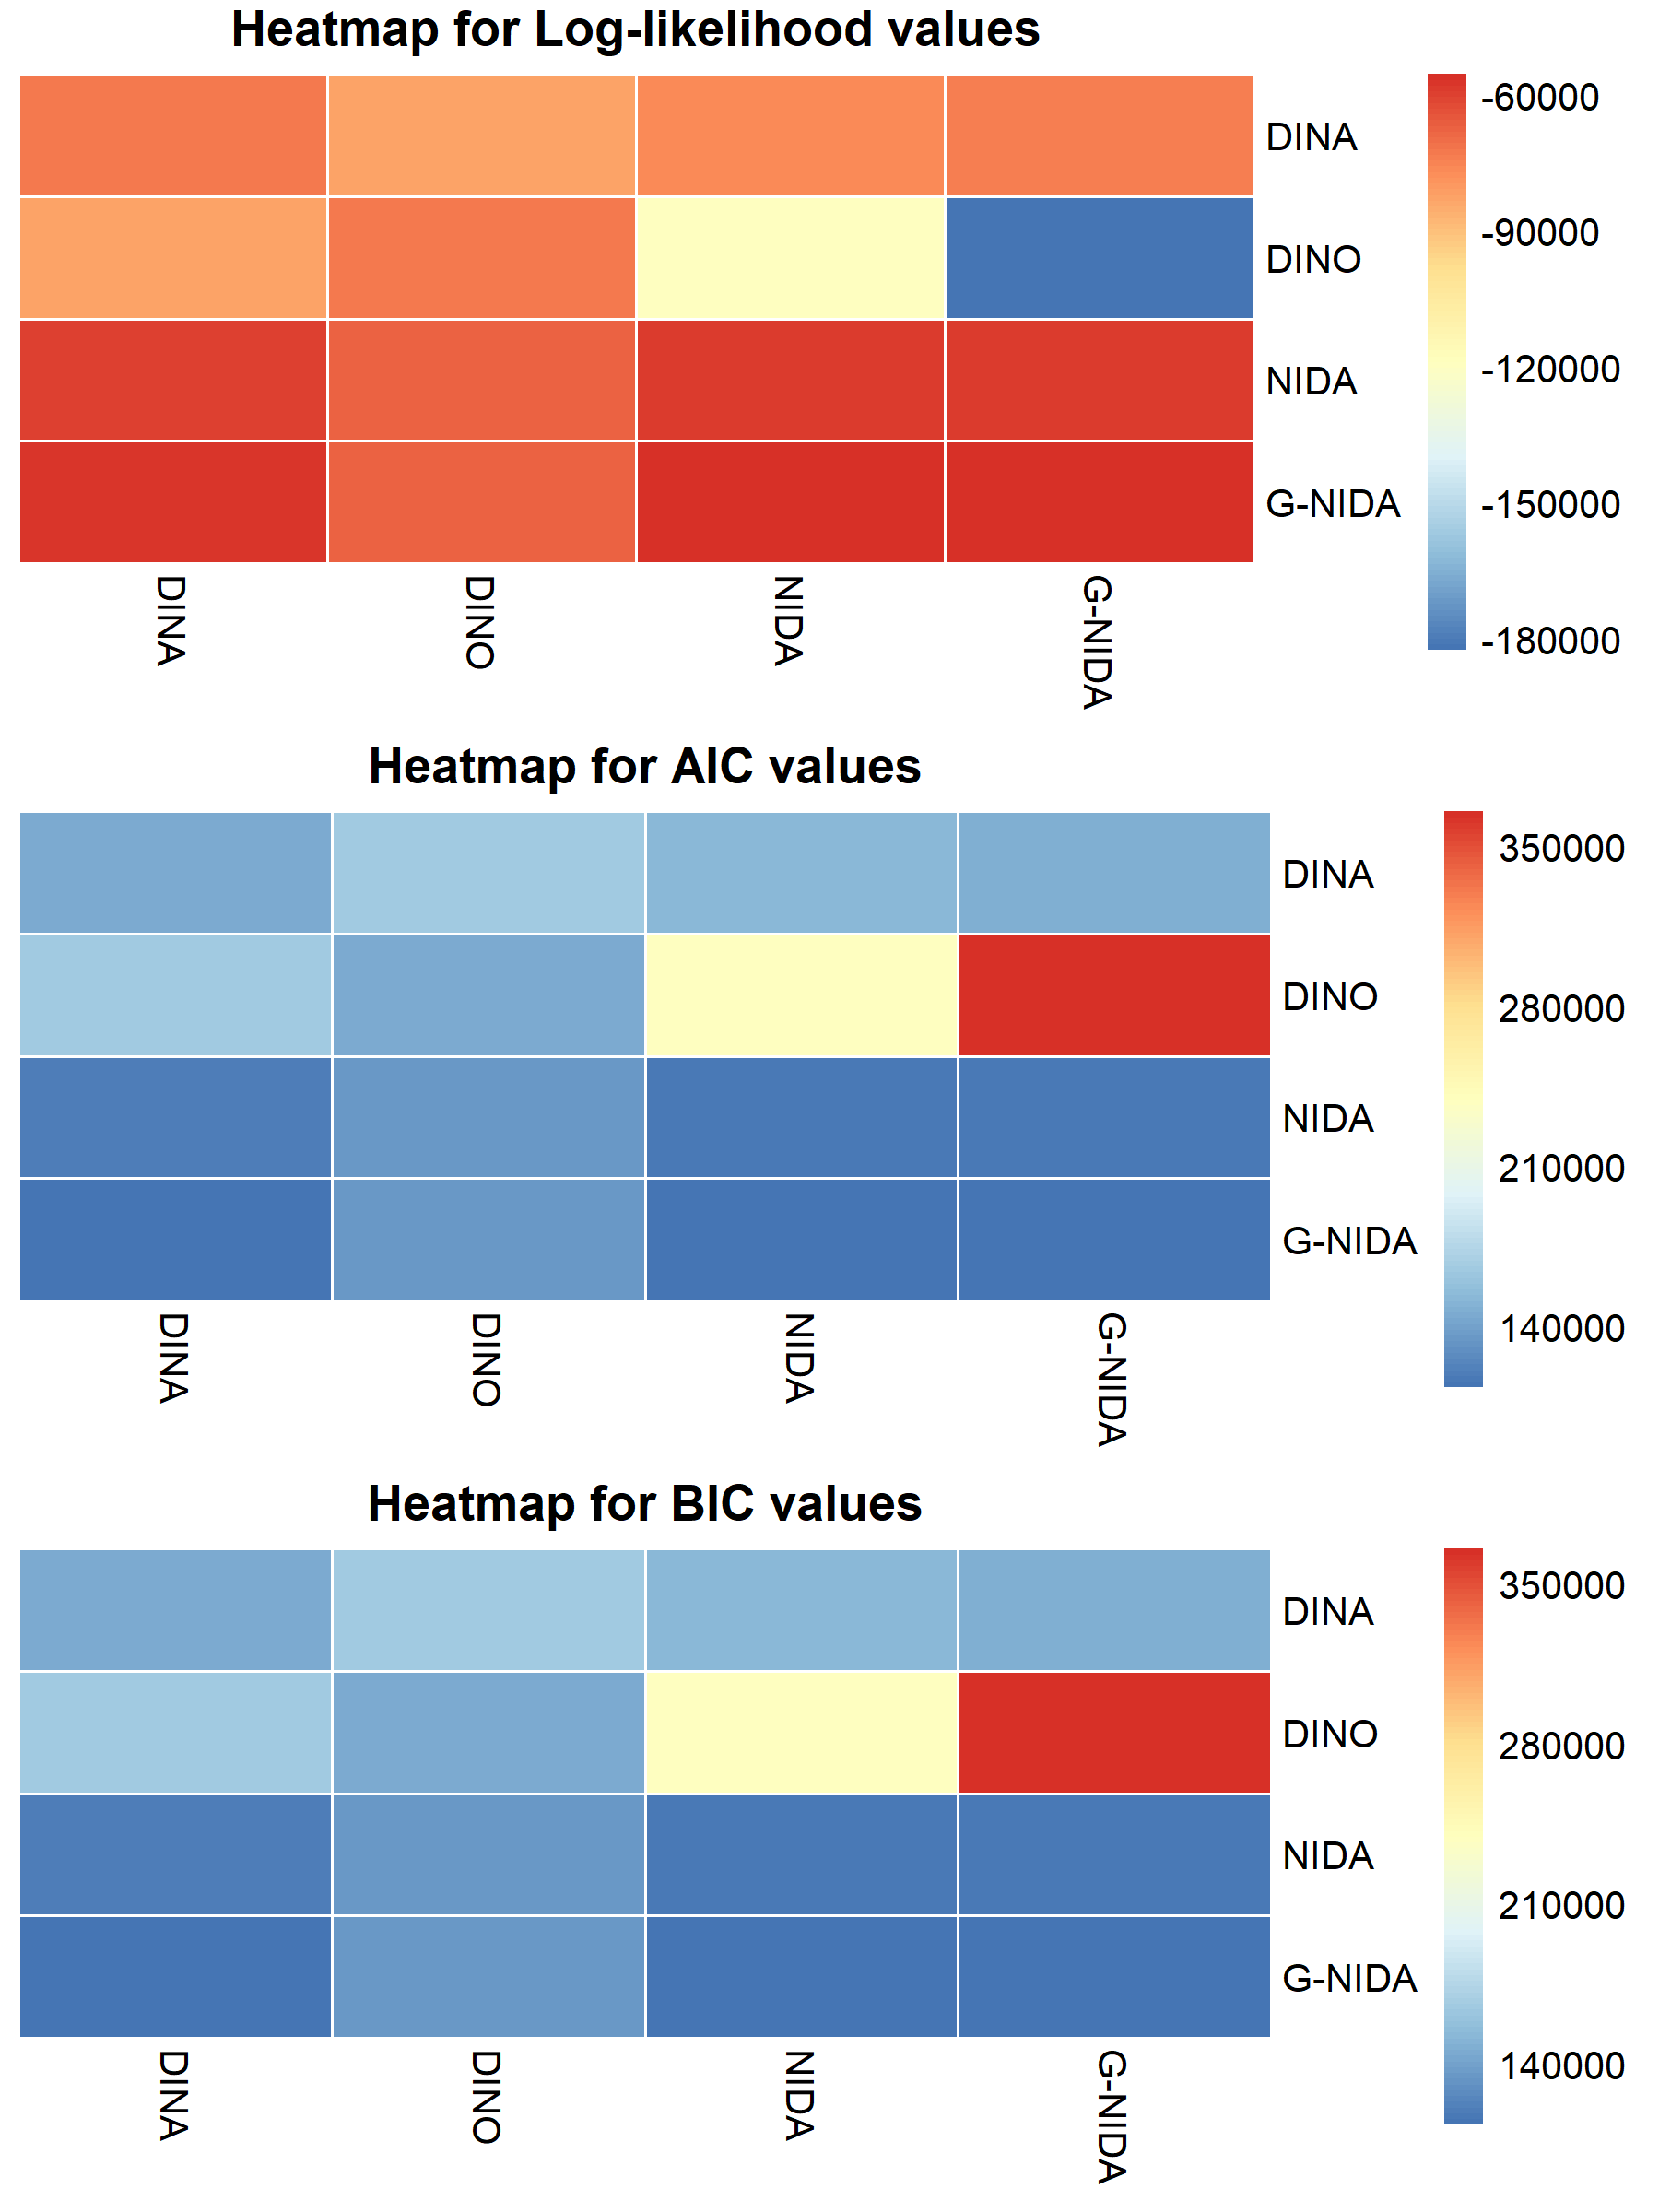
\includegraphics[width=0.7\textwidth]{Heatmaps_relative_fit.png}
		\caption{Heatmaps for log-likelihood, AIC and BIC statistics.}
		\label{heatmap_stats}
	\end{figure}
	
	The first part of the second component is examination how many skill profiles of the examinees were estimated correctly, how many profiles had four, three, two, one or none of the five skills identified correctly. The model is good when it classifies most of the skills correctly. Figures \ref{comparison_dina}, \ref{comparison_dino}, \ref{comparison_nida} and \ref{comparison_gnida} on pages \pageref{comparison_dina} and \pageref{comparison_gnida} show the number of examinees with an amount of well-classified skills for the DINA, DINO, NIDA, G-NIDA models as a~true model respectively. In the upper left corner of each barplot there is a weighted mean value that allows assessing how many skills on average are correctly determined by the model. In each case, the number of all skills classified correctly was the highest for true models and the percentage was between 64\% and 72\%. Next conclusions are also similar as in the previous case. DINA, NIDA and G-NIDA models are good fits for each other (when the model used for simulation is one of them), the difference in the weighted means is not greater than 0.1. When the response data obtained from the DINA model were estimated by DINO model and when for the true DINO model the data were estimated by DINA model, only around 15\% of skill profiles were classified fully correct. The results when the true model was DINO, for NIDA and G-NIDA models estimation were even worse and amounted to less than 6\%. None of the estimated models (except the true DINO model) classified on average more than 3.8 skills.
	
	\begin{figure}[h!]
		\centering
		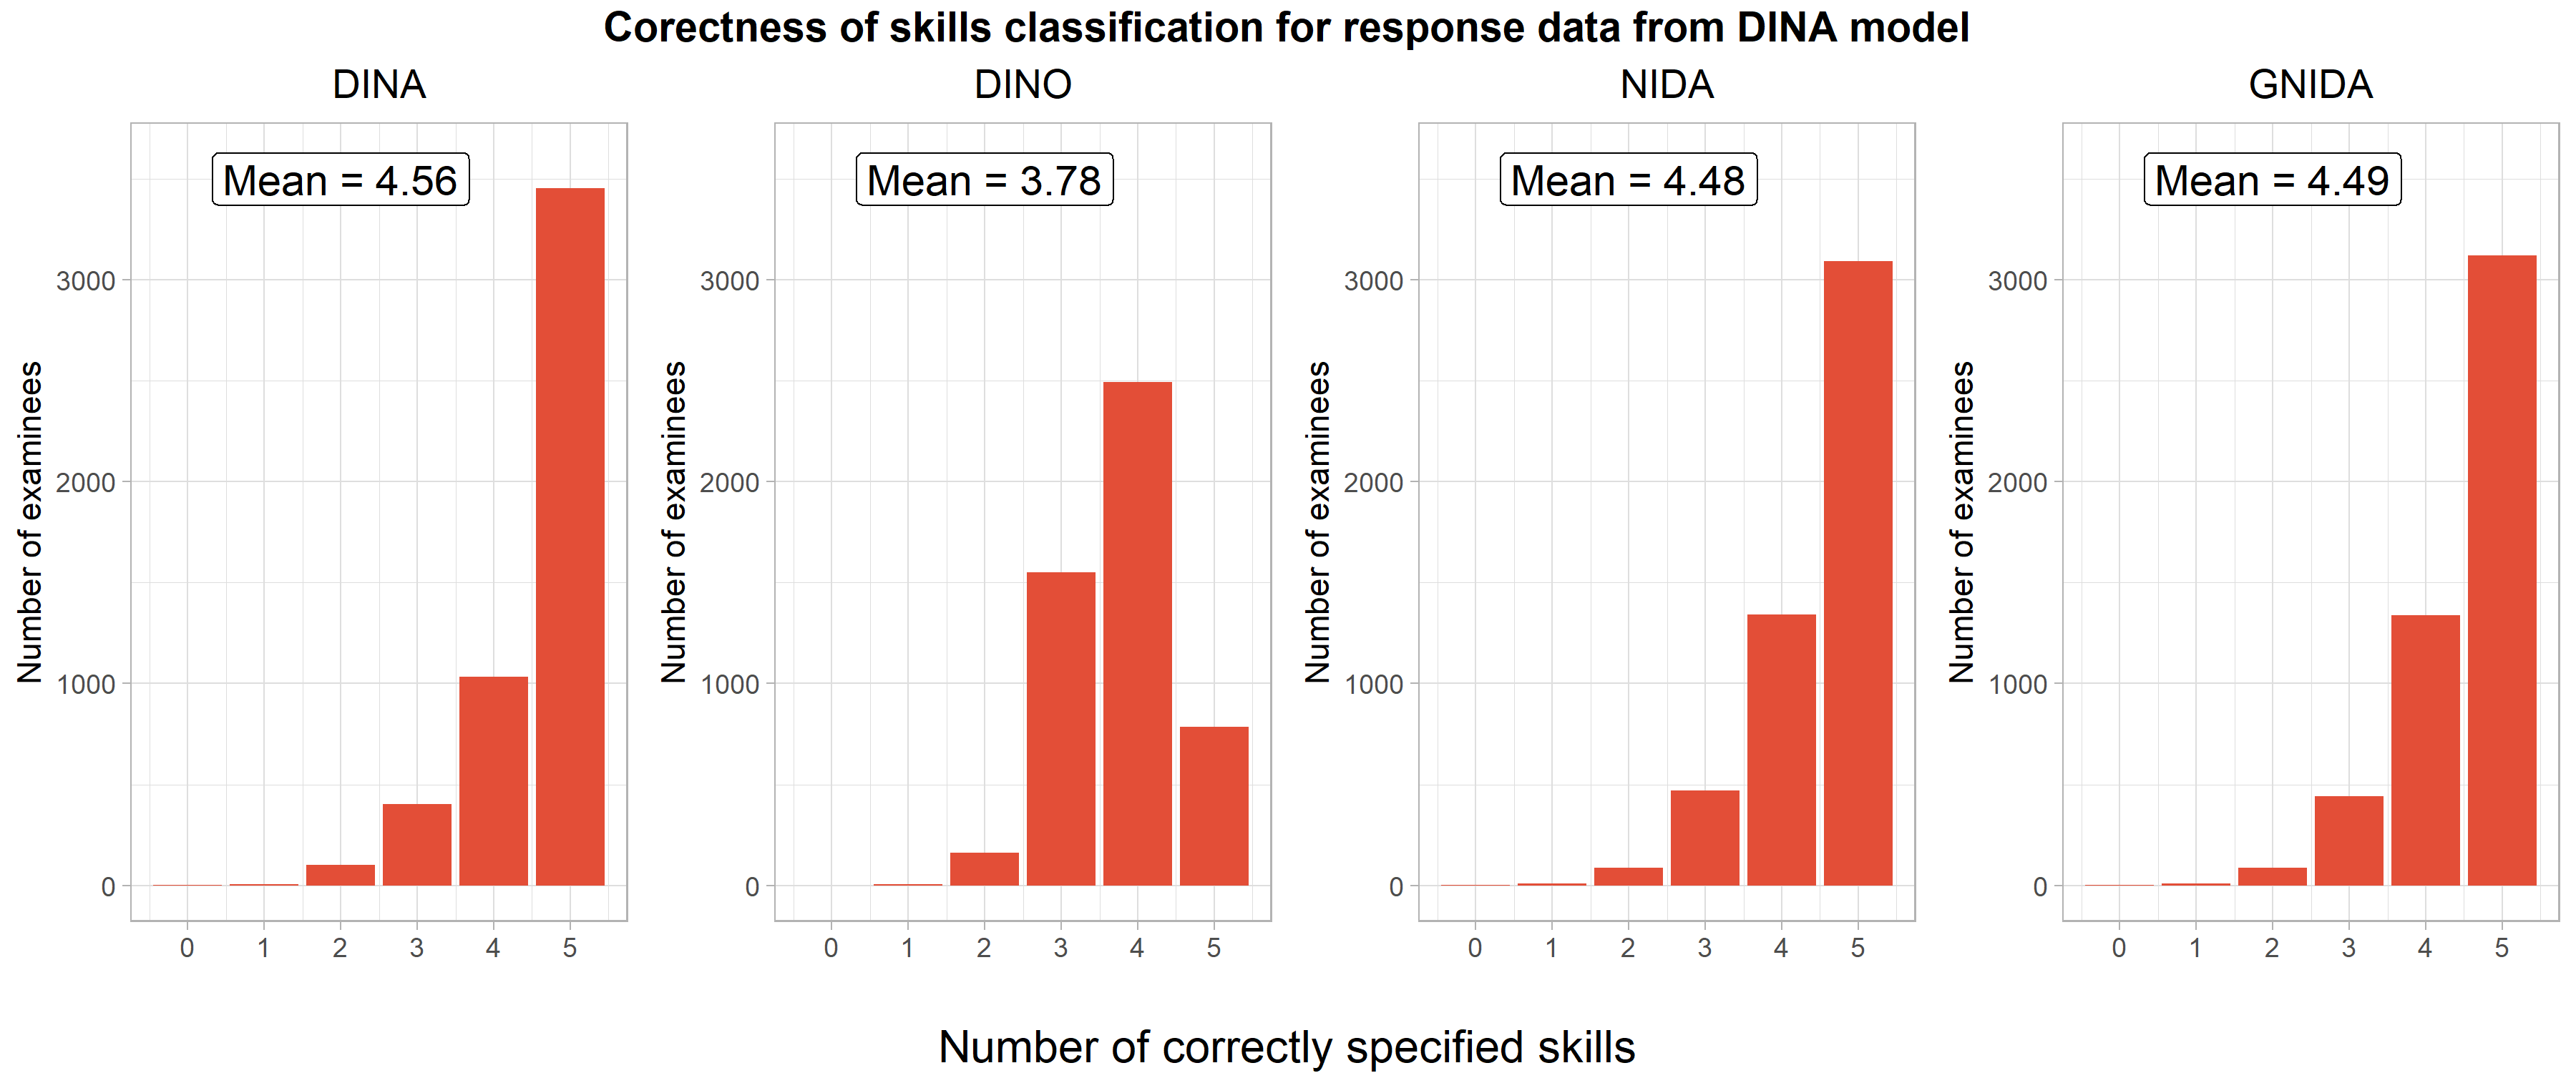
\includegraphics[width=\textwidth]{DINA_skills_classification_col.png}
		\caption{Comparison of results for the DINA model simulated.}
		\label{comparison_dina}
	\end{figure}
	
	\begin{figure}[h!]
		\centering
		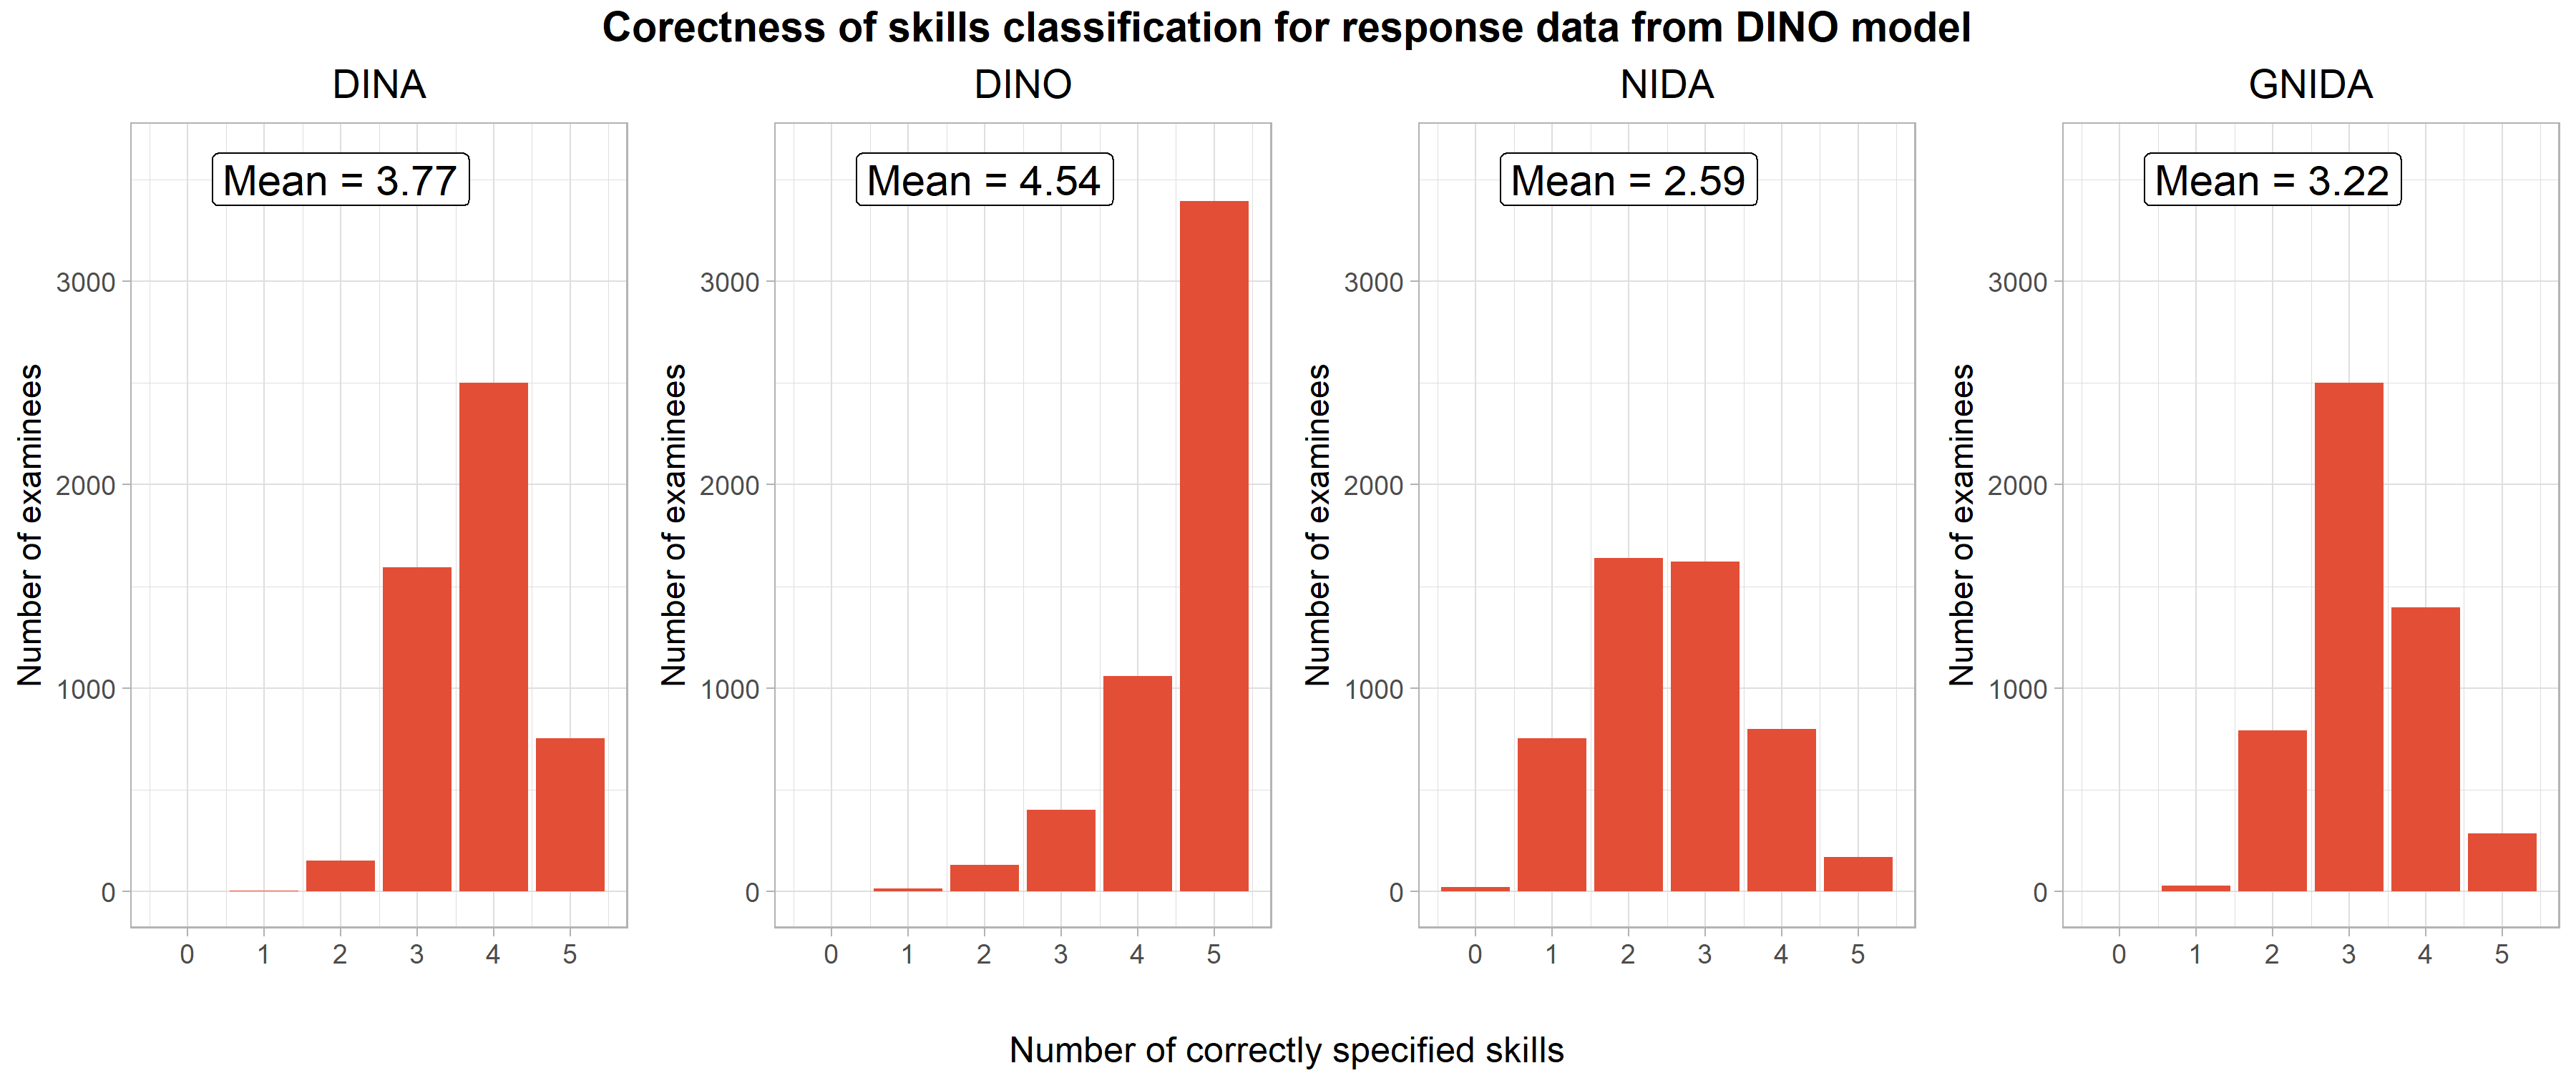
\includegraphics[width=\textwidth]{DINO_skills_classification_col.png}
		\caption{Comparison of results for the DINO model simulated.}
		\label{comparison_dino}
	\end{figure}
	
	\begin{figure}[h!]
		\centering
		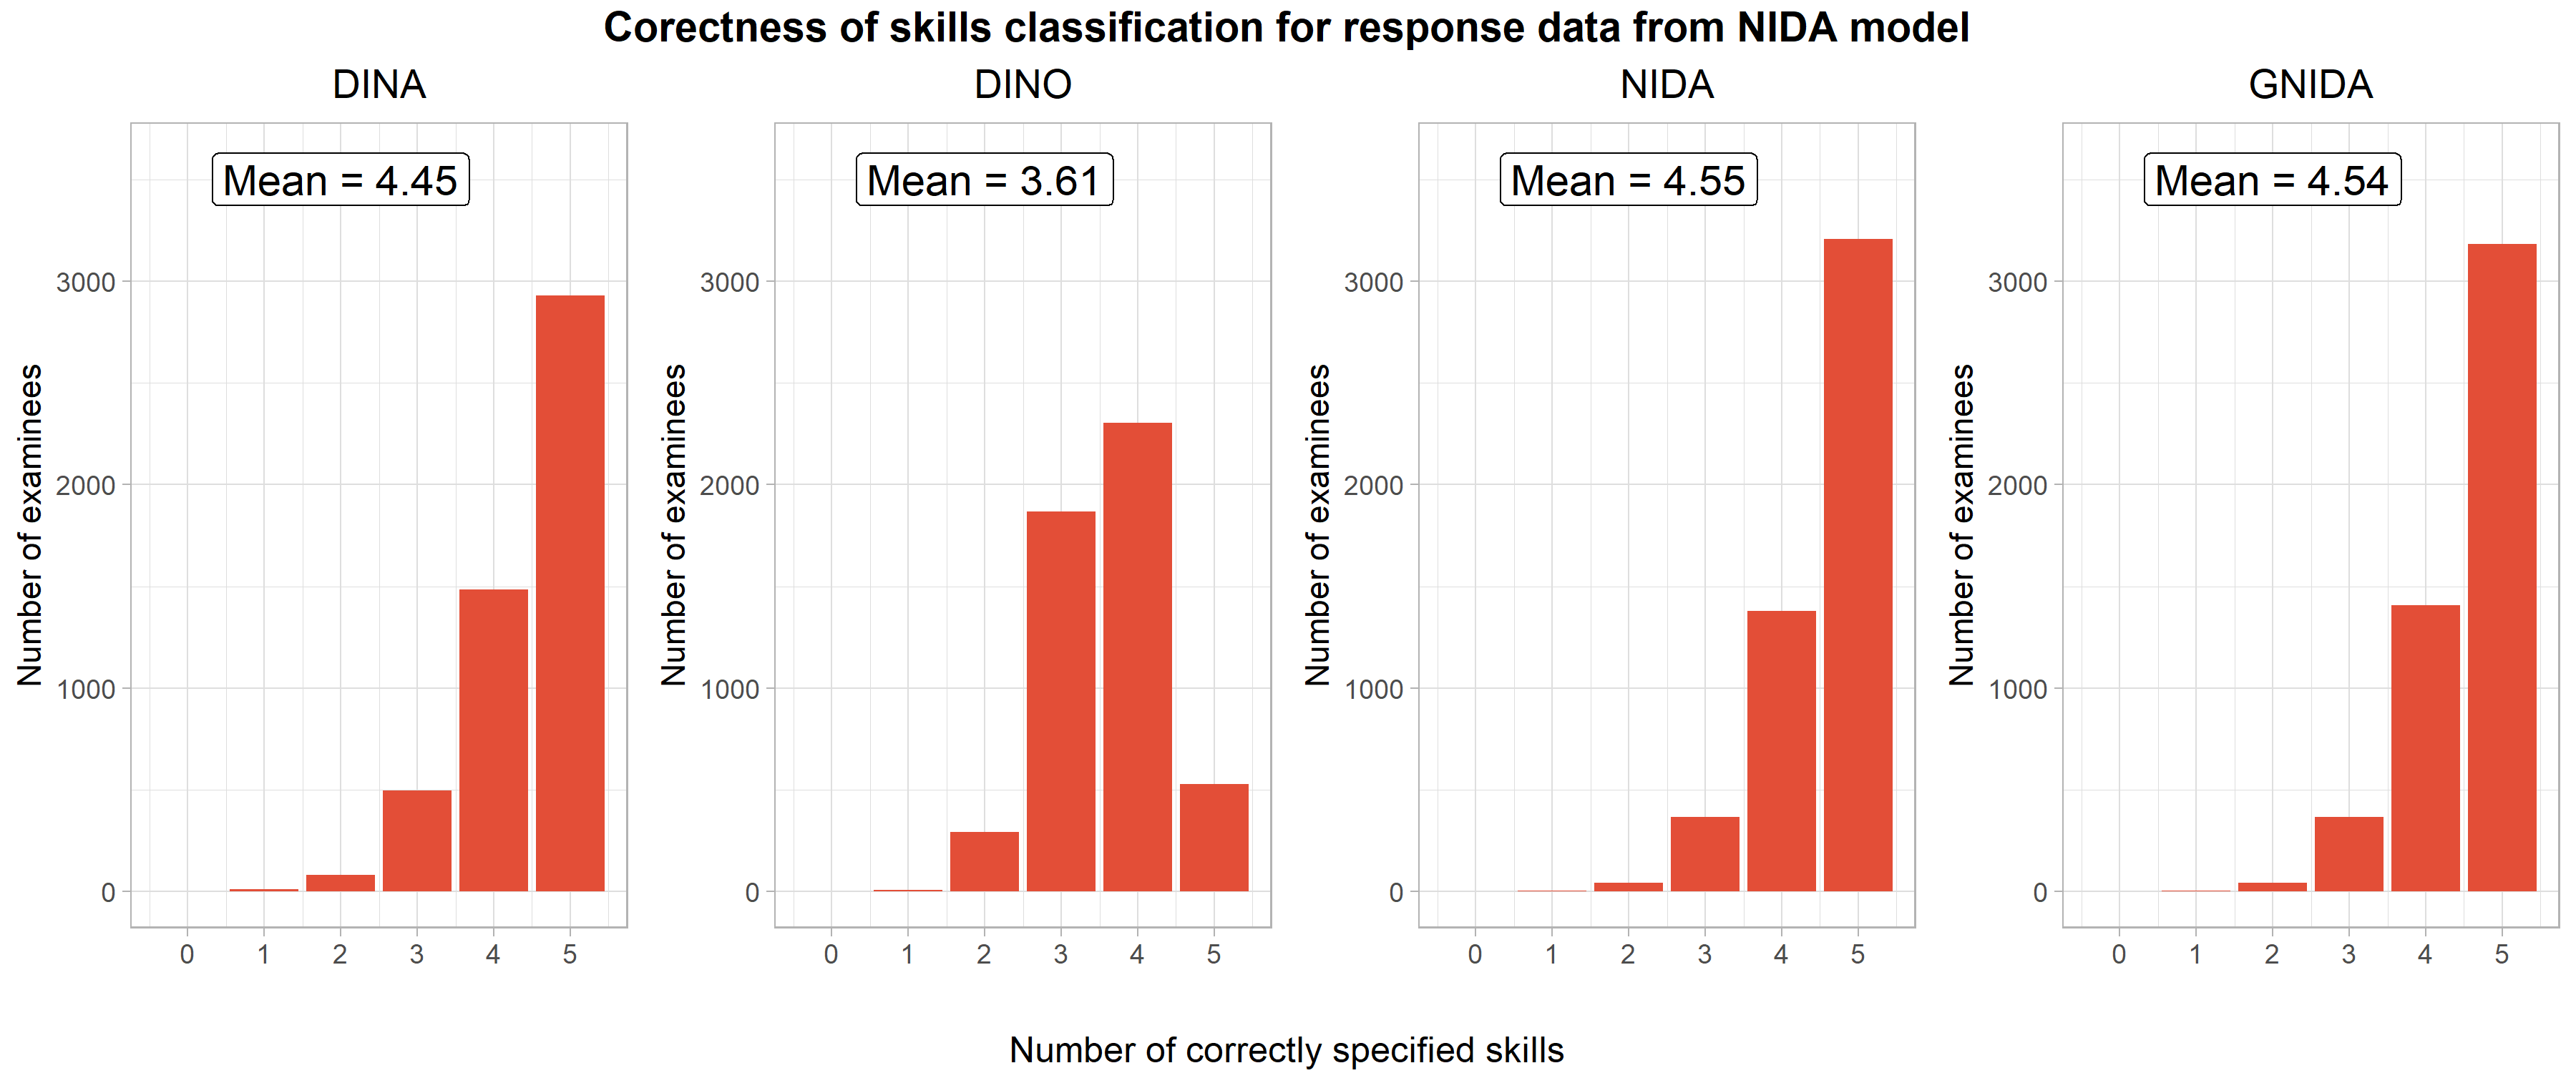
\includegraphics[width=\textwidth]{NIDA_skills_classification_col.png}
		\caption{Comparison of results for the NIDA model simulated.}
		\label{comparison_nida}
	\end{figure}
	
	\begin{figure}[h!]
		\centering
		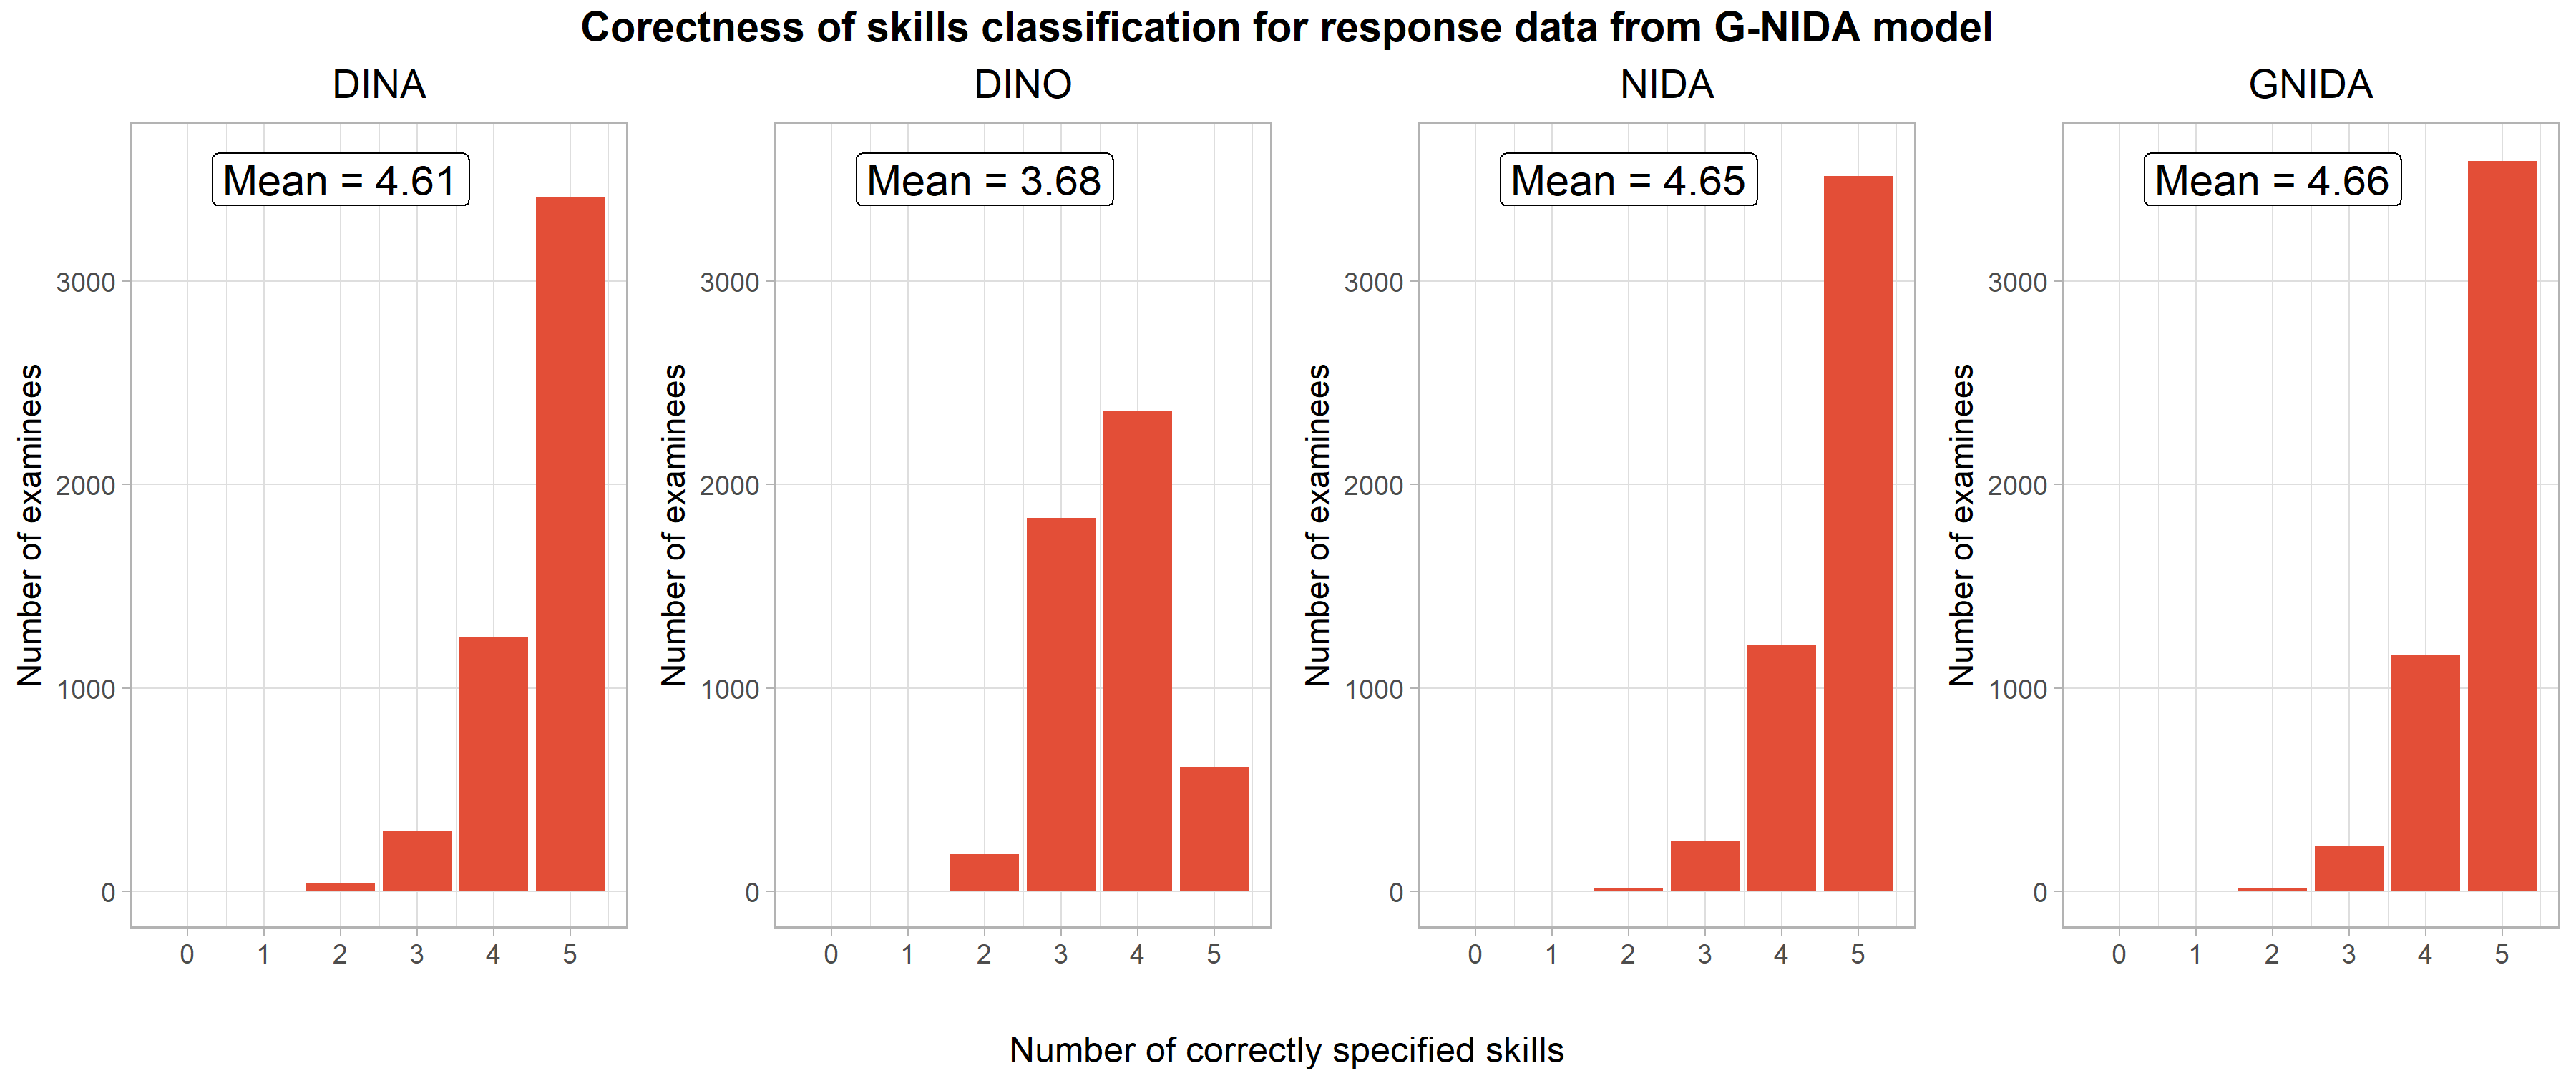
\includegraphics[width=\textwidth]{GNIDA_skills_classification_col.png}
		\caption{Comparison of results for the G-NIDA model simulated.}
		\label{comparison_gnida}
	\end{figure}
	
	The second part of the second component was examining the accuracy of the estimated models -- how often skills are well defined. Accuracies for each skill and for whole response data were obtained and the results are presented in Table \ref{tab:estimation_skills} on page \pageref{tab:estimation_skills}. Comparison of results for individual skills does not give any special conclusions, there is no pattern corresponding to the specific skill nor model. This means that models check all of the skills at a similar level. If the $Q$-matrix is well-created, there should be no dependencies of results for individual skills on estimation. Accuracies calculated for models, in general, are presented in the last column. There is no surprise that for the true model the skills are more often well defined. The results for all of the models confirm the conclusions received in the previous part.
	
	\begin{table}[H]
		\centering
		\begin{tabular}{l c c c c c c} 
			\hline
			{\rule{0pt}{3ex}} & \multicolumn{6}{c}{DINA model} \\ 
			& $\alpha_1$ & $\alpha_2$ & $\alpha_3$ & $\alpha_4$ & $\alpha_5$ & \textbf{mean} \\ [0.5ex]
			\hline 
			{\rule{0pt}{3ex}}DINA & 0.9098 & 0.9090 & 0.9216 & 0.9116 & 0.9116 & \textbf{0.91272} \\ 
			DINO & 0.7522 & 0.7680 & 0.7316 & 0.7764 & 0.7504 & \textbf{0.75572} \\
			NIDA & 0.8948 & 0.9010 & 0.9030 & 0.8908 & 0.8944 & \textbf{0.89680} \\
			G-NIDA & 0.8958 & 0.9058 & 0.9048 & 0.8930 & 0.8952 & \textbf{ 0.89892} \\ [0.5ex] 
			\hline
			{\rule{0pt}{3ex}} & \multicolumn{6}{c}{DINO model} \\ 
			& $\alpha_1$ & $\alpha_2$ & $\alpha_3$ & $\alpha_4$ & $\alpha_5$ & \textbf{mean} \\ [0.5ex]
			\hline 
			{\rule{0pt}{3ex}}DINA & 0.7358 & 0.7722 & 0.7522 & 0.7588 & 0.7496 & \textbf{0.75372} \\ 
			DINO & 0.9054 & 0.9034 & 0.9080 & 0.9072 & 0.9140 & \textbf{0.90760} \\
			NIDA & 0.5084 & 0.5180 & 0.5284 & 0.5158 & 0.5156 & \textbf{0.51724} \\
			G-NIDA & 0.6076 & 0.6814 & 0.5664 & 0.6218 & 0.7474 & \textbf{ 0.64492} \\ [0.5ex] 
			\hline
			{\rule{0pt}{3ex}} & \multicolumn{6}{c}{NIDA model} \\ 
			& $\alpha_1$ & $\alpha_2$ & $\alpha_3$ & $\alpha_4$ & $\alpha_5$ & \textbf{mean} \\ [0.5ex]
			\hline 
			{\rule{0pt}{3ex}}DINA & 0.8914 & 0.8908 & 0.8908 & 0.8870 & 0.8876 & \textbf{0.88952} \\ 
			DINO & 0.7446 & 0.7276 & 0.7120 & 0.7130 & 0.7132 & \textbf{0.72208} \\
			NIDA & 0.9098 & 0.9154 & 0.9072 & 0.9032 & 0.9128 & \textbf{0.90968} \\
			G-NIDA & 0.9078 & 0.9144 & 0.9070 & 0.9038 & 0.9104 & \textbf{ 0.90868} \\ [0.5ex] 
			\hline
			{\rule{0pt}{3ex}} & \multicolumn{6}{c}{G-NIDA model} \\ 
			& $\alpha_1$ & $\alpha_2$ & $\alpha_3$ & $\alpha_4$ & $\alpha_5$ & \textbf{mean} \\ [0.5ex]
			\hline 
			{\rule{0pt}{3ex}}DINA & 0.9108 & 0.9106 & 0.9272 & 0.9248 & 0.9316 & \textbf{0.92100} \\ 
			DINO & 0.7496 & 0.7148 & 0.7262 & 0.7544 & 0.7364 & \textbf{0.73628} \\
			NIDA & 0.9180 & 0.9186 & 0.9378 & 0.9380 & 0.9334 & \textbf{0.92916} \\
			G-NIDA & 0.9206 & 0.9240 & 0.9398 & 0.9402 & 0.9404 & \textbf{ 0.93300} \\ [0.5ex] 
			\hline
		\end{tabular}
		\caption{Mean values of skills classification for each model.}
		\label{tab:estimation_skills} 
	\end{table}
	
	The last part of the second component concerning an absolute fit evaluation for CDM misspecification is examining informedness (which determines how well-informed the test is relative to randomness), markedness (which determines how well the population is tested against randomness) and their geometric mean -- correlation (which describes how much the results of the method are correlated with the actual assessment). The results are presented in Table \ref{tab:confusion_values} (page \pageref{tab:confusion_values}) and in Figure \ref{heatmap_measures} (page \pageref{heatmap_measures}), which includes the heatmaps for each measure. The values obtained for these measures are more diverse than previously. For example, the value of the informedness for the NIDA model, when the true model was DINO, is very low -- less than 3\%, which results in the correlation, between the estimation and real response data, equal to about 12\%. The informedness value equal to 0 means complete randomness, so the result obtained for the NIDA model is very unfavorable and suggests that if there are any indications for the real data that DINO is the correct model (for example, there are many ways to solve the item), then the NIDA model should not be used for estimation. However, all of the results confirm previous conclusions -- measures have the highest values for the true models, have similar results for all of the non-compensatory models and have the worst values for NIDA and G-NIDA models, when the true model is DINO.
	
	\begin{table}[H]
		\centering
		\begin{tabular}{l l c c c c} 
			\hline
			{\rule{0pt}{3ex}} \multirow{2}{*}{True model} & \multirow{2}{*}{Measure} & \multicolumn{4}{c}{Estimated models} \\\cmidrule{3-6}
			& & DINA & DINO & NIDA & G-NIDA \\ [0.5ex]
			\hline 
			{\rule{0pt}{3ex}} \multirow{3}{*}{DINA model} & informedness & \textbf{0.8253833} & 0.5140384 & 0.7936219 & 0.7978157 \\ 
			& markedness & \textbf{0.8255185} & 0.6198476 & 0.7935927 & 0.7978475 \\ 
			& correlation & \textbf{0.8254509} & 0.5644692 & 0.7936073 & 0.7978316\\ 
			[0.5ex] 
			\hline
			{\rule{0pt}{3ex}} \multirow{3}{*}{DINO model} & informedness & 0.5048264 & \textbf{0.8152497} & 0.0284173 & 0.2858251 \\ 
			& markedness & 0.6141829 & \textbf{0.8152247} & 0.5103258 & 0.4896448 \\ 
			& correlation & 0.5568265 & \textbf{0.8152372} & 0.1204246 & 0.3741026\\ 
			[0.5ex] 
			\hline
			{\rule{0pt}{3ex}} \multirow{3}{*}{NIDA model} & informedness & 0.7795057 & 0.4474721 & \textbf{0.8195347} & 0.8175810 \\ 
			& markedness & 0.7832871 & 0.6204171 & \textbf{0.8199320} & 0.8183015 \\ 
			& correlation & 0.7813941 & 0.5268960 & \textbf{0.8197333} & 0.8179412\\ 
			[0.5ex] 
			\hline
			{\rule{0pt}{3ex}} \multirow{3}{*}{G-NIDA model} & informedness & 0.8421491 & 0.4757360 & 0.8585197 & \textbf{0.8662798} \\ 
			& markedness & 0.8424090 & 0.6394361 & 0.8590959 & \textbf{0.8675957} \\ 
			& correlation & 0.8422790 & 0.5515458 & 0.8588077 & \textbf{0.8669375}\\ 
			[0.5ex] 
			\hline
		\end{tabular}
		\caption{Values of measures for different models.}
		\label{tab:confusion_values} 
	\end{table}
	
	\begin{figure}[ht!]
		\centering
		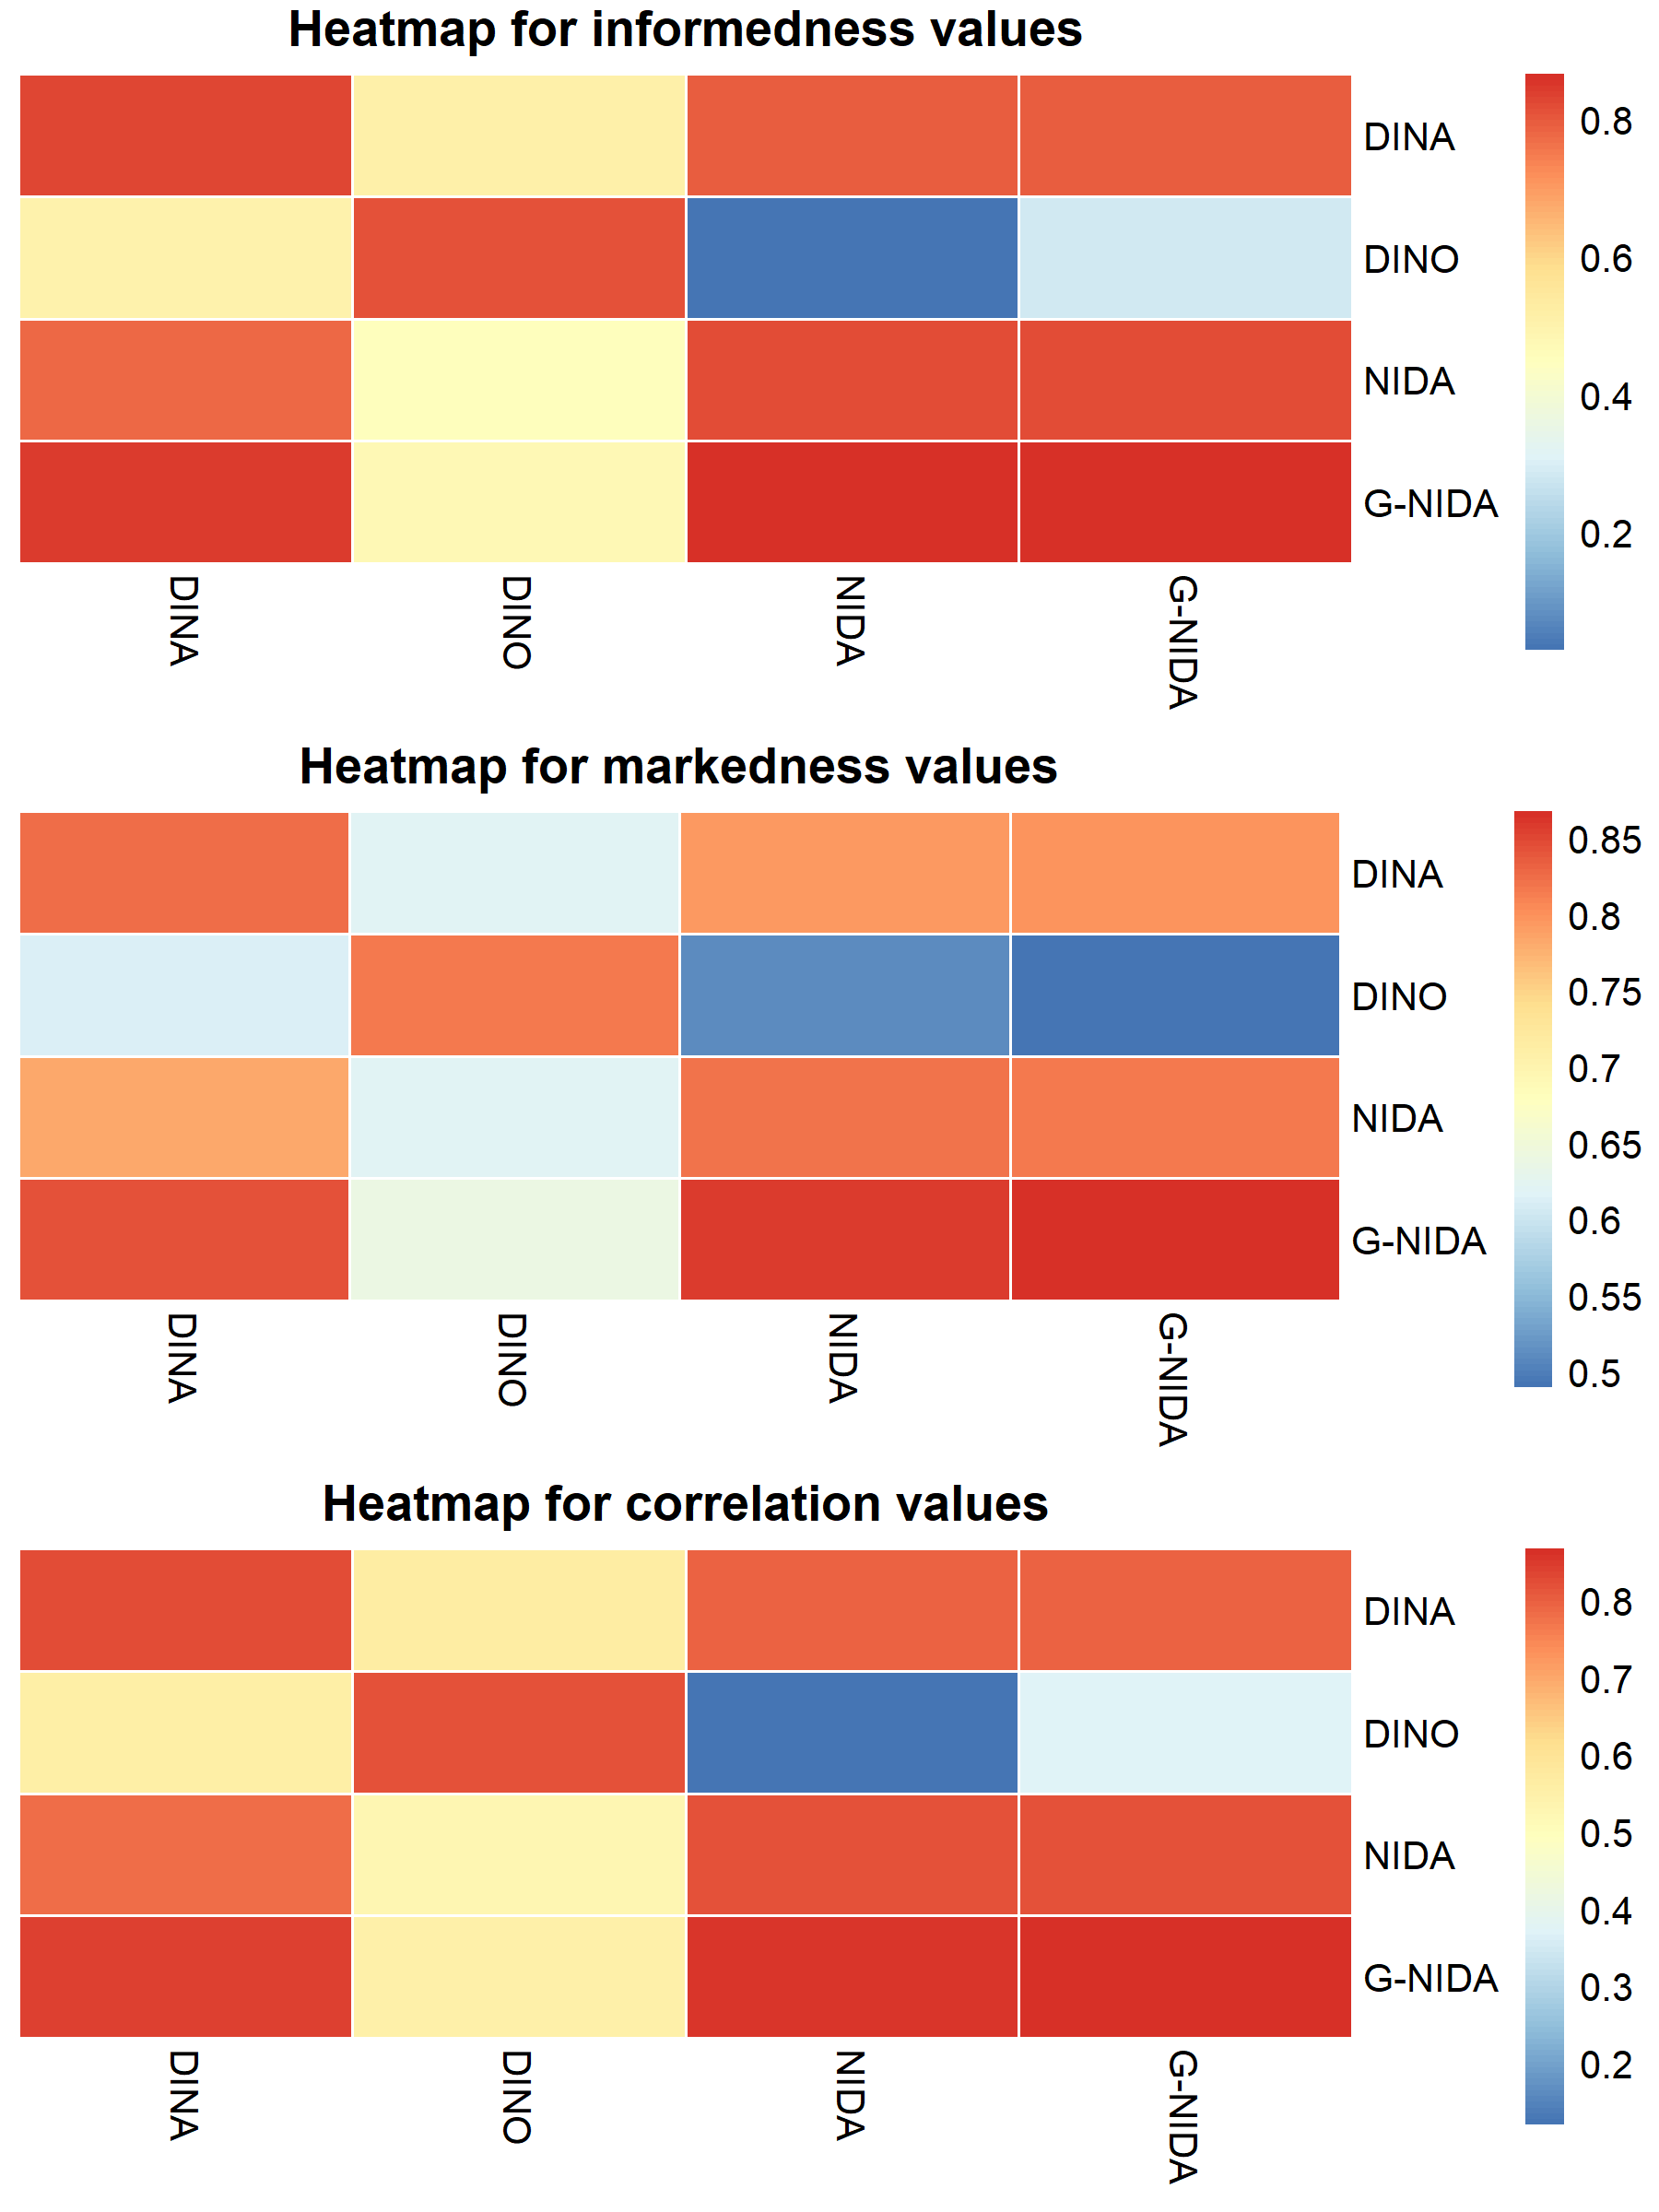
\includegraphics[width=0.7\textwidth]{Heatmaps_absolute_fit.png}
		\caption{Heatmaps for informedness, markedness and correlation measures.}
		\label{heatmap_measures}
	\end{figure}
	
	Summarizing, after comparing the results of the estimation with the results for the simulation using the true model, all of the statistics and measures returned the best values for the true model. Obtained results mean that all of the models were good enough to fit the data correctly. Estimating the response data with the use of the DINO model for DINA, NIDA and G-NIDA as a true model, gave the worst results. The possible reason for this situation is the type of the group to which this model belongs -- the DINO is an example of the compensatory model, while the other three belong to the non-compensatory group. G-NIDA is a saturated model -- is more general, so theoretically and practically it is a good fit for other models from the same group (DINA and NIDA models). However, G-NIDA model application requires more complex computations. The DINA model, which is much easier than G-NIDA, also obtained very good results and it is the best fit for the DINO model (which is in a group of non-compensatory models) that is why it is going to be used in Section \ref{section:qmat_misspec}.
	
	
	
	%%%%%%%%%%%%%%%%%%%%%%%%%%%%%%%%%%%%%%%%%%%%%%%%%%%%%%%%%%%%%%%%%%%%%%%%%%%%%%%%%%%%%%%%%%%%%%%%%%%%%%%%%%%%%
	
	\newpage
	\section{Q-matrix misspecification}\label{section:qmat_misspec}
	
	This simulation was conducted to check whether the $Q$-matrix misspecification has a~significant impact on the estimation results. The following factors were manipulated in the simulation: the type of the $Q$-matrix misspecification (overspecified, underspecified and both \cite{m2statistic} as well as randomly generated and fragmentarily permuted) and the size of the response data (the number of examinees). Two numbers of rows in the response data were considered: $I = 1000$ and $I =5000$. Thus, a total of 14 conditions resulted after combining all of the cases. The number of items was fixed at $J=30$ and the number of attributes was fixed at $K=5$. The examinees’ attribute patterns were generated using the uniform distribution and their responses were simulated under the DINA model (according to results obtained in Section \ref{section:cdm_misspec}). The slipping and guessing parameters were set to $0.2$. For the estimation \texttt{gdina()} function was used, which allows estimating the DINA model. It is not possible to estimate NIDA or G-NIDA models with \texttt{gdina()} function, that is why it could not be used earlier. The \texttt{gdina()}, the same as the \texttt{JMLE()} function, maximizes the log-likelihood function, but it is much faster, so choosing it is more efficient. A total of 100 data sets were generated for each of the conditions to eliminate any substantial Monte Carlo error.
	
	The correct $Q$-matrix used to generate the data is the same as for the CDM misspecification and it is given in Table \ref{tab:qmatrix_sim} on page \pageref{tab:qmatrix_sim}. The $Q$-matrix has an equal number of 1-, 2- and 3-attribute items, and each attribute is measured by the same number of items. Its structure satisfies the required conditions to be an identifiable \cite{qmat_identifiability} and complete \cite{qmat_complete} $Q$-matrix. 
	
	The types of misspecifications in the $Q$-matrix can be divided into two groups. In the first group (concerning overspecification, underspecification and both), misspecifications were introduced randomly with two constraints: first, all items measure at least one skill, and second, none of the items measures more than three skills. The number of misspecified vectors in $Q$-matrix is equal to 6 which is 20\% of all $q$-vectors. Overspecified matrix was obtained by choosing vectors from first 10 rows in $Q$-matrix, the underspecified matrix was obtained by choosing vectors from last 10 rows, and for overspecified and underspecified $Q$-matrix, vectors were chosen from all possible. 
	
	Misspecifications in the $Q$-matrix in the second group consisted in the total random generation of the $Q$-matrix as well as the selection of a fragment of the $Q$-matrix (first ten, first twenty or all of the vectors) and a random displacement of them in the matrix. All of the results obtained during simulations were compared with the results for the correct $Q$-matrix.
	
	
	\subsection{Results}
	
	As in Section \ref{section:cdm_misspec}, the first component of $Q$-matrix misspecification evaluation concerns a~relative fit evaluation. In Tables \ref{tab:estimations_qmat} and \ref{tab:estimations_qmat2} (page \pageref{tab:estimations_qmat2}) are presented results of examining log-likelihood values, AIC and BIC statistics for the length of the response matrix equal to $I=1000$ and $I=5000$, respectively. Because of the relativity of statistics, it is no possible to compare the results between different numbers of examinees, but it is possible to compare results for different types of misspecifications. However, the conclusions are the same for both numbers of examinees'. There is no surprise that in both cases the highest log-likelihood value and the lowest Akaike and Bayesian information criteria were obtained for a correct $Q$-matrix. Analyzing first group of misspecifications, it can be noticed that the model with the underspecified matrix did the best. This is important information for the teacher, because it says that when it is not clear what skills are needed for a given item, it is better to consider fewer than more. Analyzing second group of misspecifications, it can be seen right away that the results are much worse than for the first group. The reason for these results is that none of the skills were properly defined (the permutation was performed on all 10 first $q$-vectors that required only one skill), while with overspecification only 6 vectors were changed. Increasing the number of permuted rows results in worse statistics' results. However, it is worth noting that the results for the permuted $Q$-matrix are very similar to the results for the randomly generated $Q$-matrix, even though the random matrix could include item requiring also 4 and 5 skills.
	
	\begin{table}[h]
		\centering
		\begin{tabular}{l c c c c} 
			\hline
			{\rule{0pt}{3ex}}Statistics & \multicolumn{4}{c}{Type of $Q$-matrix} \\ [0.5ex]
			\hline
			{\rule{0pt}{3ex}}& True & Over & Under & Both \\\cmidrule{2-5}
			log-likelihood & -17472.39 & -17994.47 & -17707.08 & -17923.88 \\ 
			AIC & 35096.79 & 36140.94 & 35566.15 & 35999.76 \\ 
			BIC & 35469.78 & 36513.93 & 35939.14 & 36372.75\\
			\hline
			{\rule{0pt}{3ex}}& Permuted 10 & Permuted 20 & Permuted 30 & Random \\\cmidrule{2-5}
			log-likelihood & -18350.02 & -18683.24 & -18743.70 & -18753.53 \\ 
			AIC & 36852.03 & 37518.48 & 37639.40 & 37659.06 \\ 
			BIC & 37225.02 & 37891.47 & 38012.39 & 38032.05\\ 
			[0.5ex] 
			\hline 
		\end{tabular}
		\caption{Values of statistics for scoring the correctness of fitting models with different $Q$-matrices for the sample size $I=1000$.}
		\label{tab:estimations_qmat} 
	\end{table}
	
	\begin{table}[h]
		\centering
		\begin{tabular}{l c c c c} 
			\hline
			{\rule{0pt}{3ex}}Statistics & \multicolumn{4}{c}{Type of $Q$-matrix} \\ [0.5ex]
			\hline
			{\rule{0pt}{3ex}}&True & Over & Under & Both \\\cmidrule{2-5}
			log-likelihood & -87656.75 & -90195.35 & -88998.36 & -89989.11 \\ 
			AIC & 175465.49 & 180542.70 & 178148.73 & 180130.21 \\ 
			BIC & 175960.80 & 181038.01 & 178644.03 & 180625.52\\
			\hline
			{\rule{0pt}{3ex}}& Permuted 10 & Permuted 20 & Permuted 30 & Random \\\cmidrule{2-5}
			log-likelihood & -92088.13 & -93881.08 & -94147.31 & -94194.13 \\ 
			AIC & 184328.27 & 187914.17 & 188446.63 & 188540.26 \\ 
			BIC & 184823.57 & 188409.47 & 188941.93 & 189035.57\\ 
			[0.5ex] 
			\hline 
		\end{tabular}
		\caption{Values of statistics for scoring the correctness of fitting models with different $Q$-matrices for the sample size $I=5000$.}
		\label{tab:estimations_qmat2} 
	\end{table}
	
	\newpage
	The second component concerns absolute fit evaluation. The first stage is examination how many skill profiles of the examinees were estimated correctly, how many profiles had four, three, two, one or none
	of the five skills identified correctly. Figures \ref{comparison_qmatrices1000} (page \pageref{comparison_qmatrices1000}) and \ref{comparison_qmatrices} (page \pageref{comparison_qmatrices}) presents results for $I=1000$ and $I=5000$ respectively. The first observation is almost identical results for different sample sizes. It means that the number of examinees does not have to be very large for the estimation results to be reliable. Again the simulation conclusions are the same for the two compared sizes of the response matrix. Worth attention are the plots for the second misspecification group. While for 10 permuted $q$-vectors the model is quite good at correctly classifying all five skills, for 20 and 30 permuted $q$-vectors, the model usually correctly classifies only three out of five skills. Surprisingly, the model with randomly generated $Q$-matrix classifies skills better than the 20 and 30 permuted $q$-vectors models.
	
	\begin{figure}[ht]
		\centering
		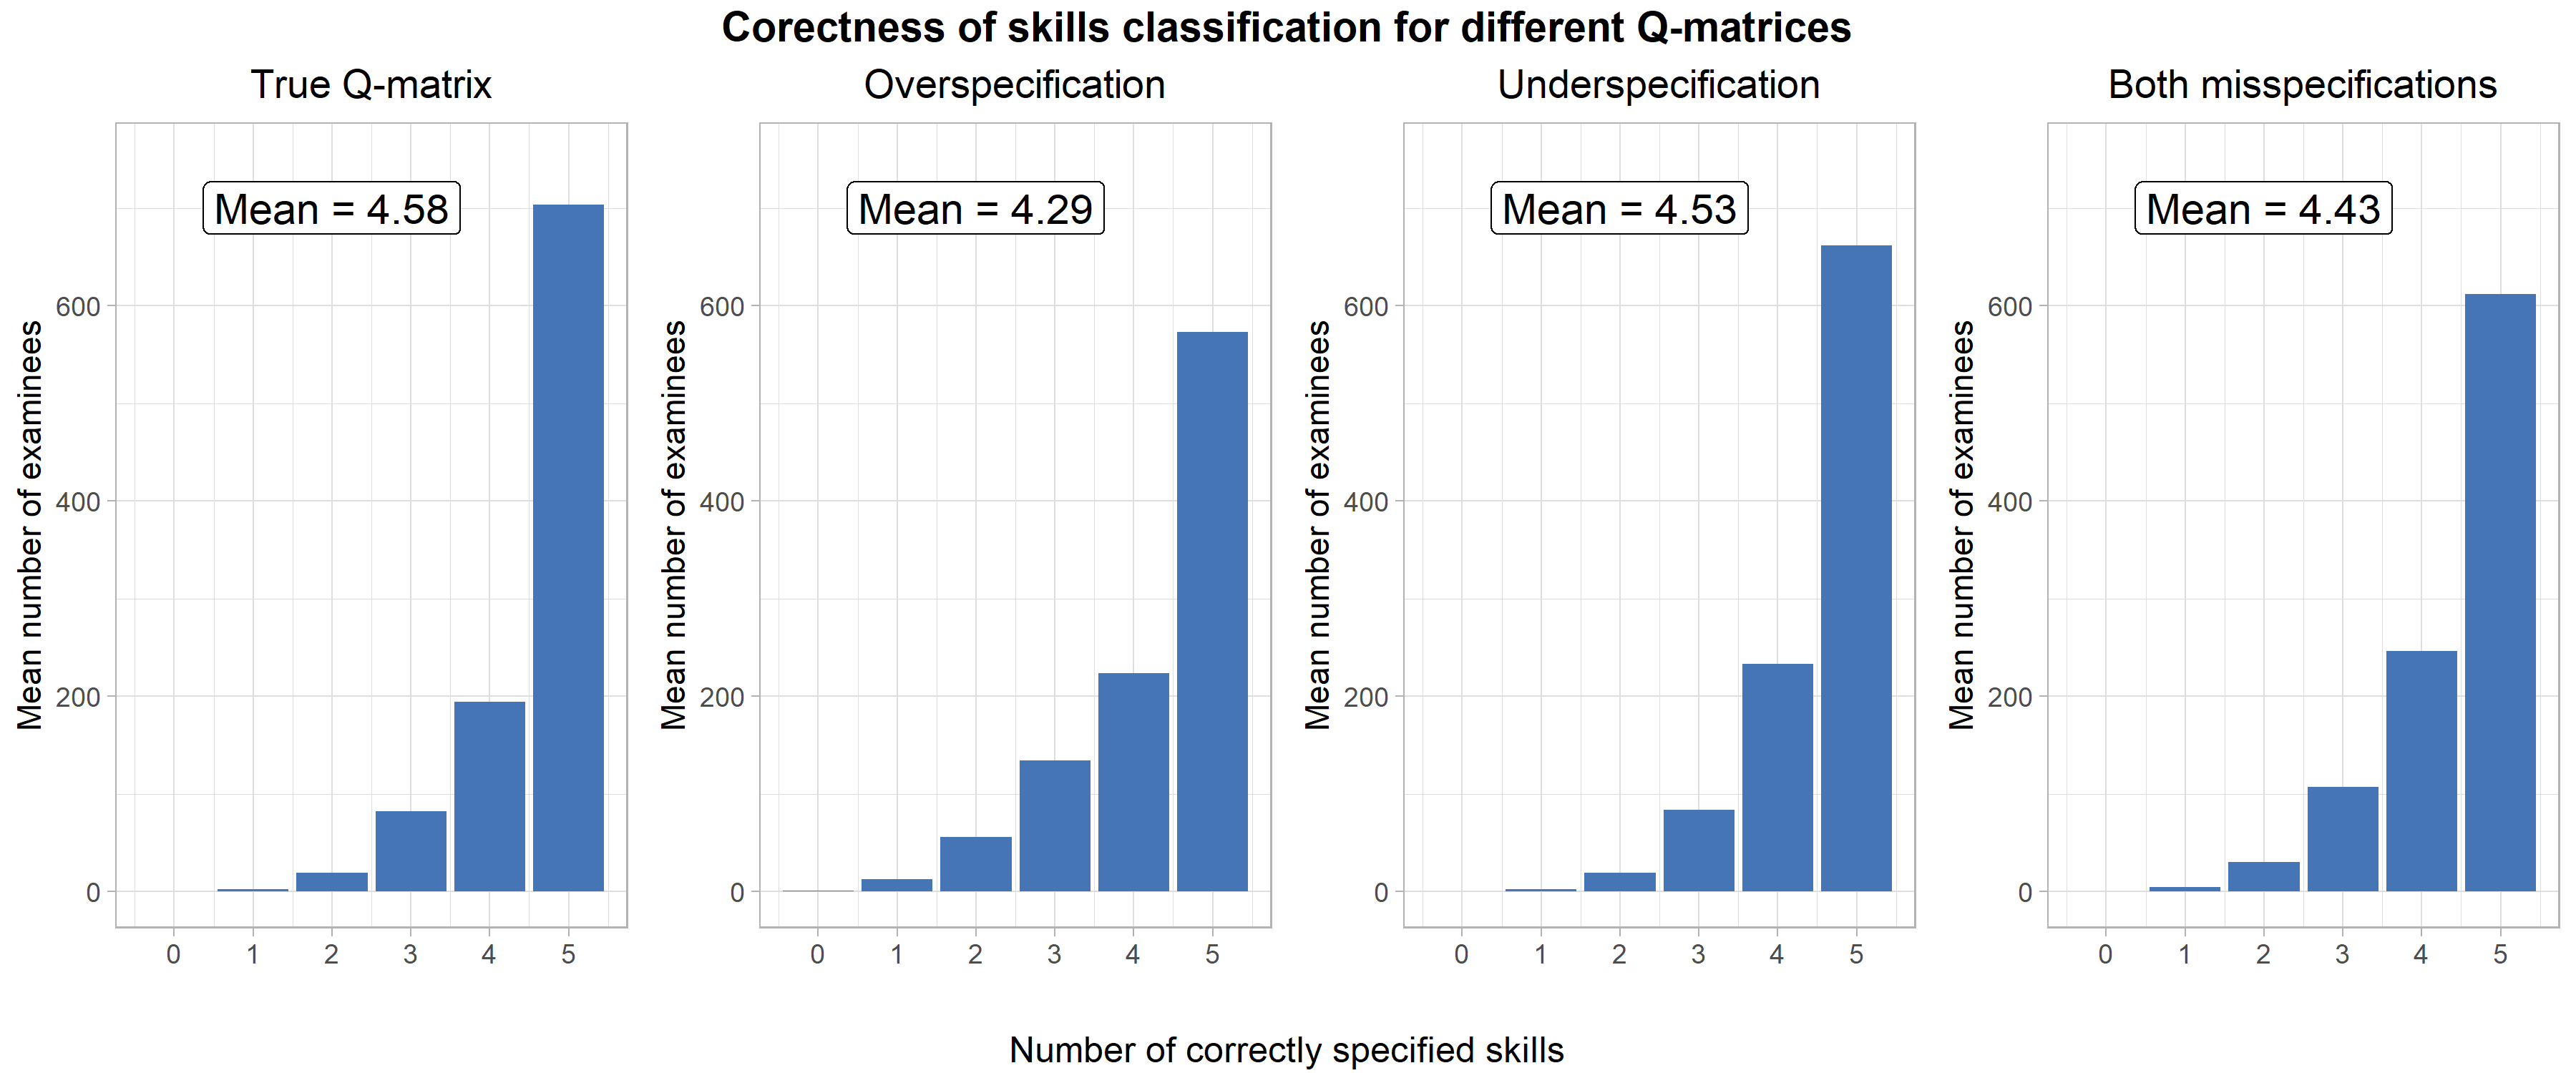
\includegraphics[width=\textwidth]{Qmat_skills_classification_1000_col.png}
		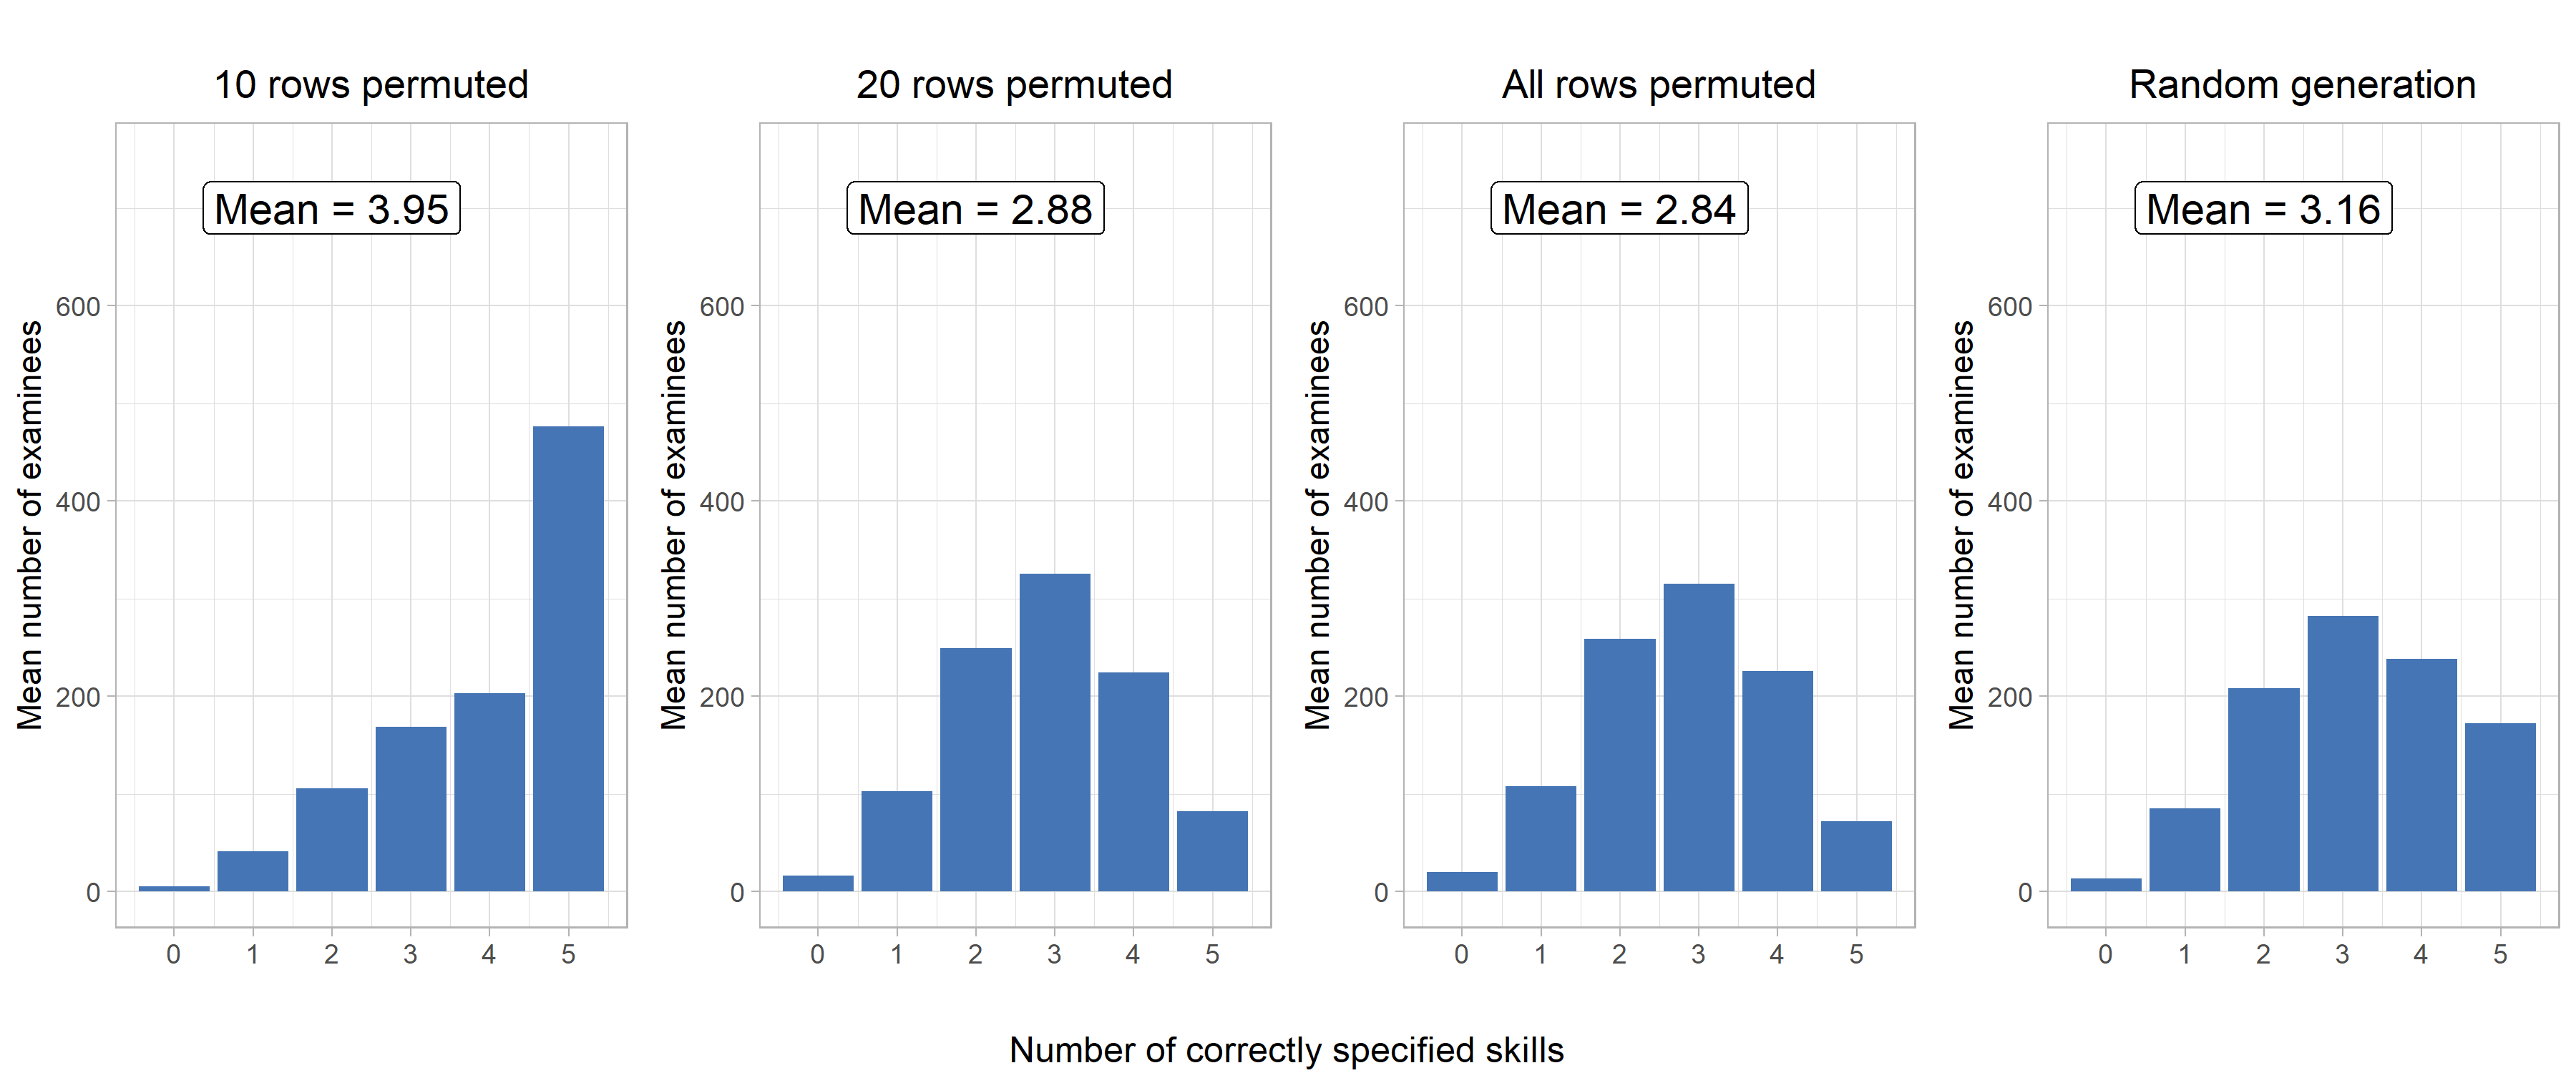
\includegraphics[width=\textwidth]{Qmat_skills_classification2_1000_col.png}
		\caption{Comparison of results for different $Q$-matrices ($I=1000$).}
		\label{comparison_qmatrices1000}
	\end{figure}
	
	\begin{figure}[ht]
		\centering
		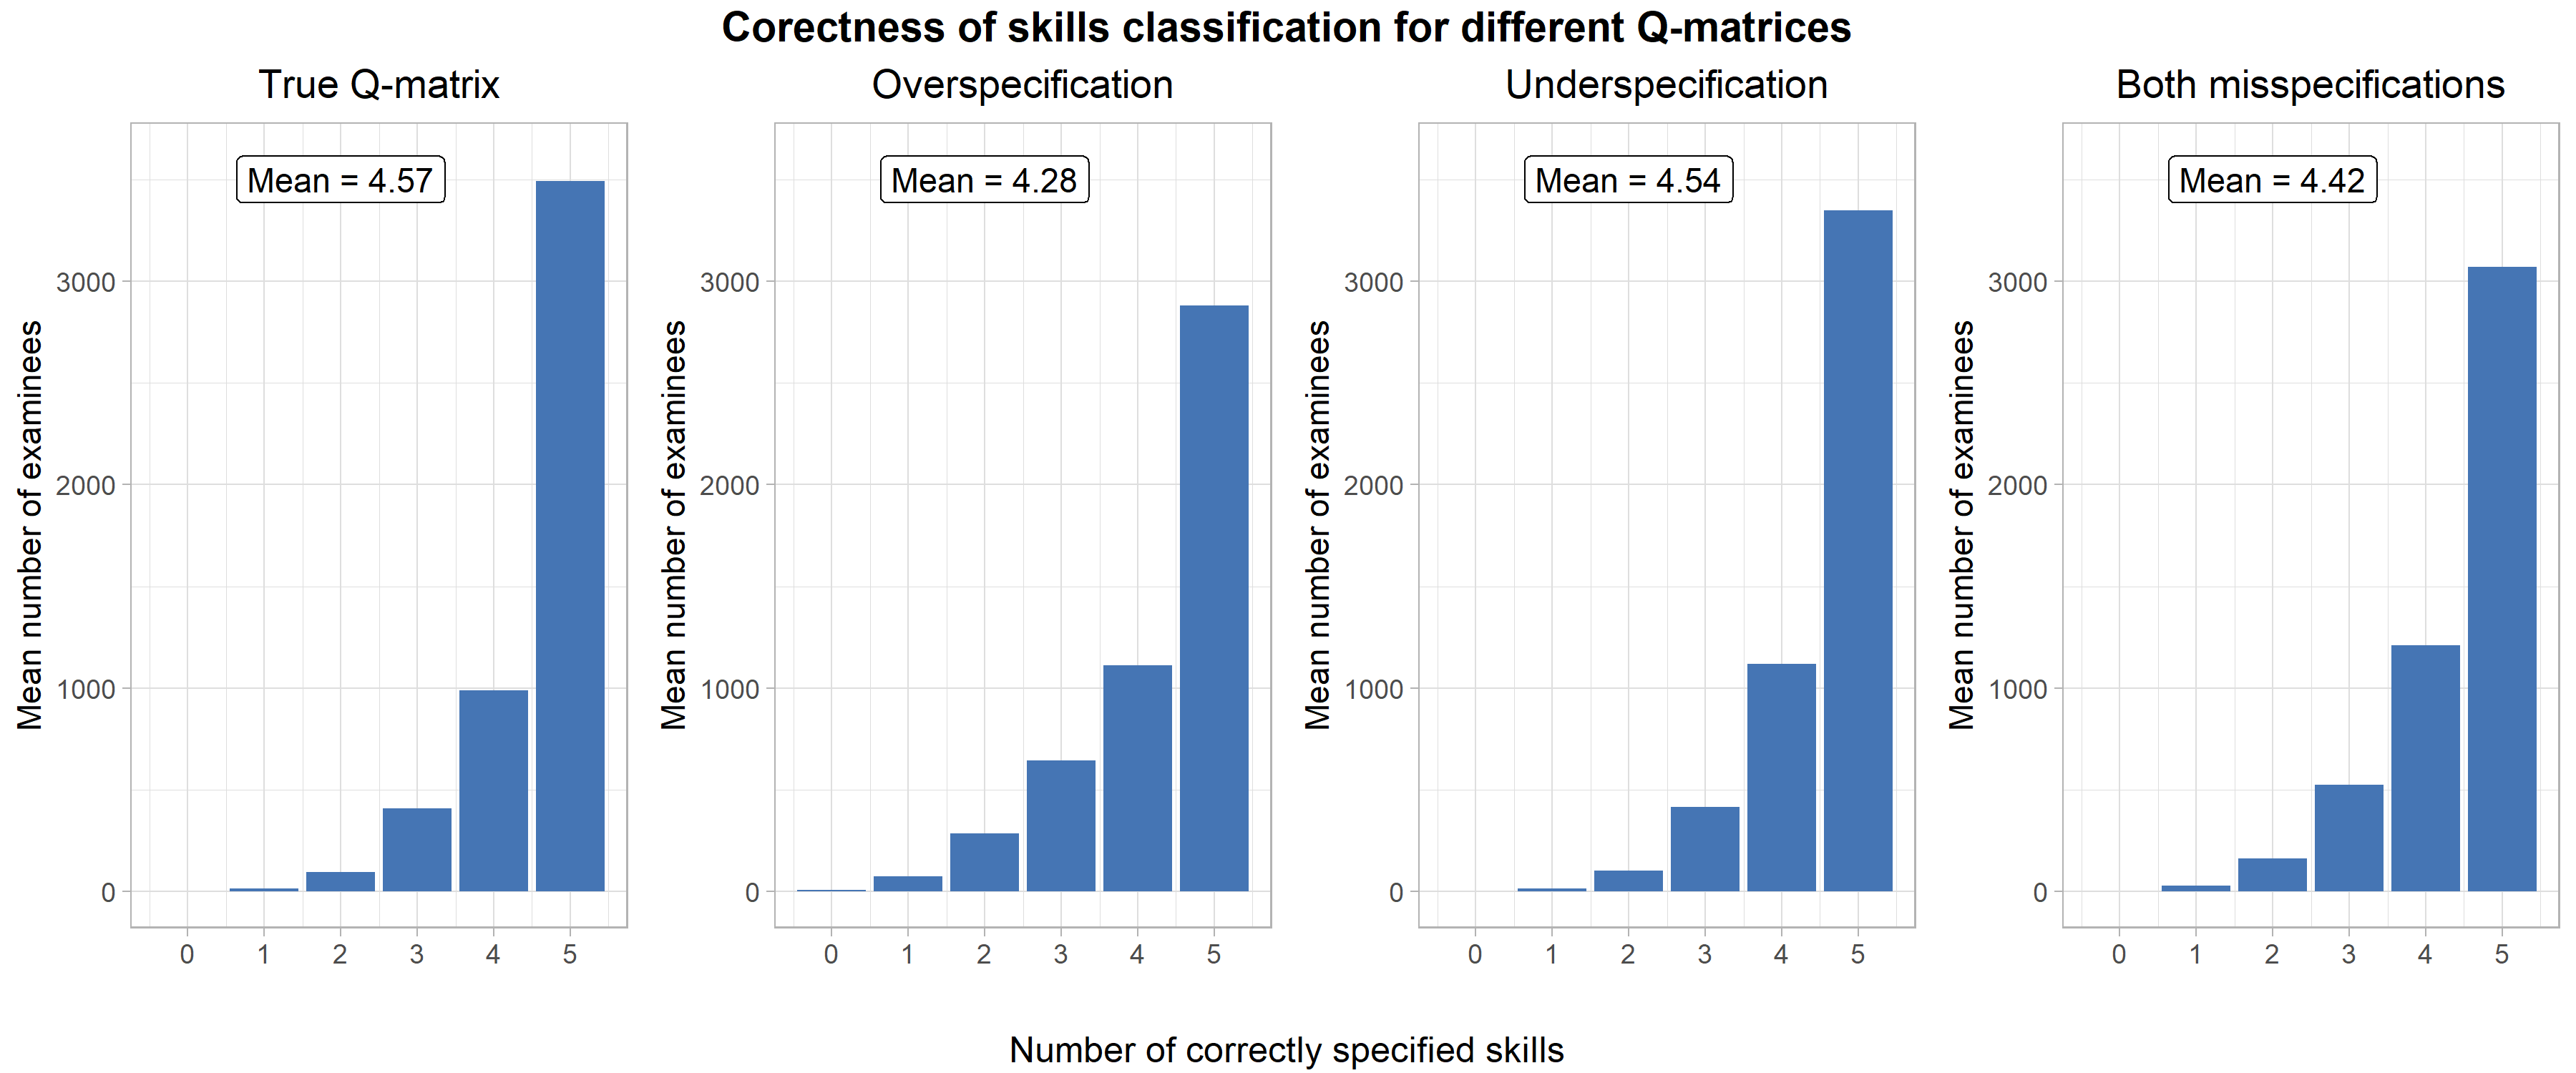
\includegraphics[width=\textwidth]{Qmat_skills_classification_5000_col.png}
		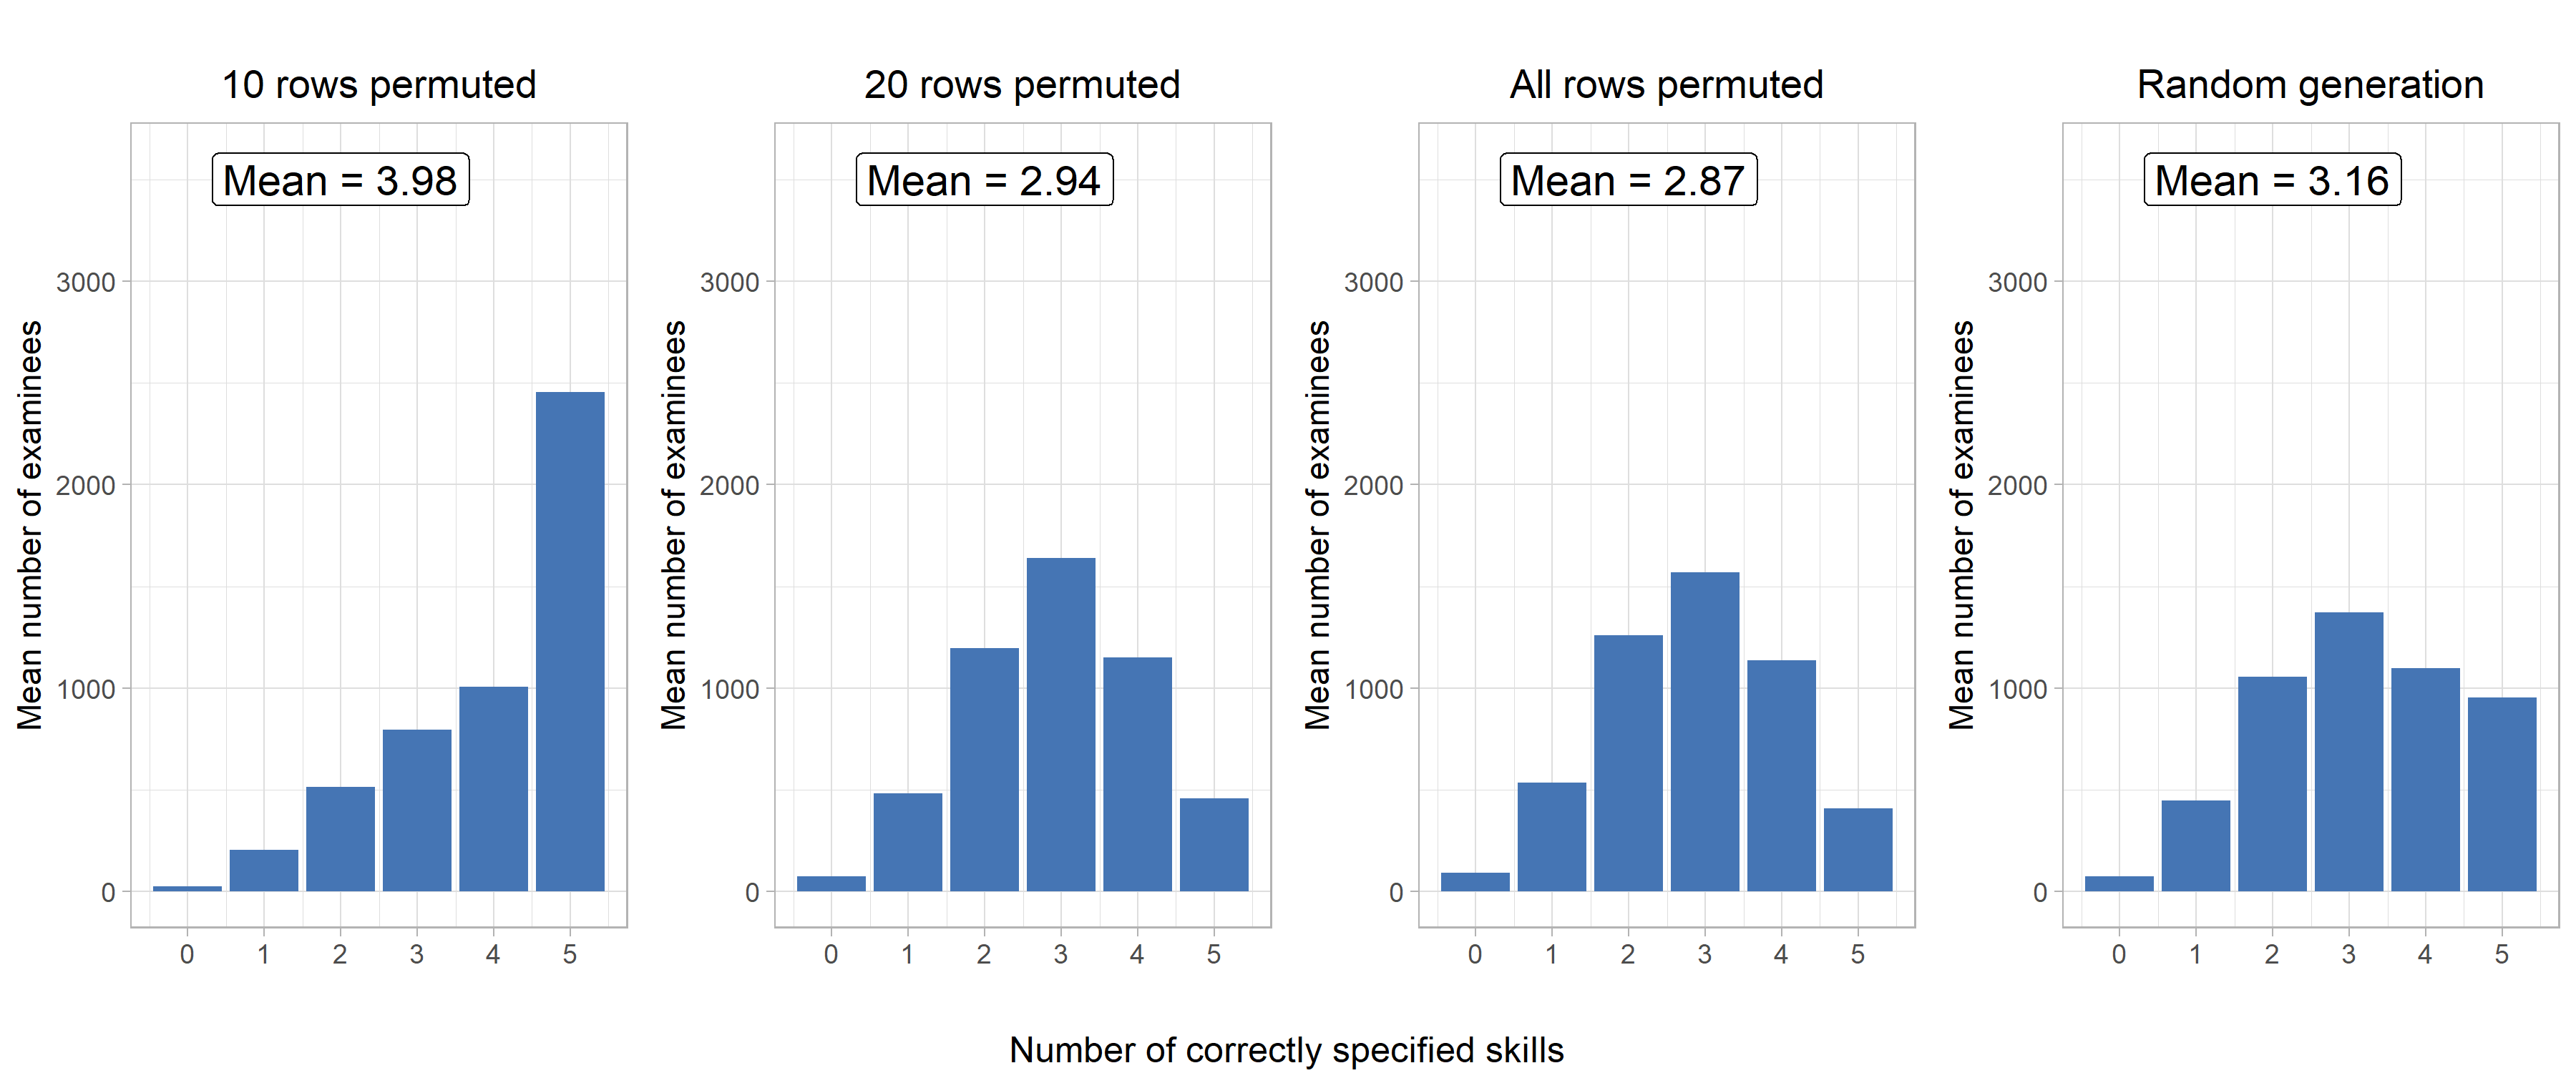
\includegraphics[width=\textwidth]{Qmat_skills_classification2_5000_col.png}
		\caption{Comparison of results for different $Q$-matrices ($I=5000$).}
		\label{comparison_qmatrices}
	\end{figure}
	
	\newpage
	Table \ref{tab:estimation_skills_qmat} on page \pageref{tab:estimation_skills_qmat} shows the percentage of how often each skill is well defined.  Accuracies calculated for different types of $Q$-matrix, for all of the skills, are presented in the last column. Comparison of results for individual skills does not give any special conclusions. This means that models check all of the skills at a similar level. The results for all of the models are the same as the conclusions received in the part concerning analysis of relative fit evaluation. 
	
	\begin{table}
		\centering
		\begin{tabular}{l c c c c c c} 
			\hline
			{\rule{0pt}{3ex}} & \multicolumn{6}{c}{$I=1000$} \\ 
			Type of $Q$-matrix & $\alpha_1$ & $\alpha_2$ & $\alpha_3$ & $\alpha_4$ & $\alpha_5$ & \textbf{mean} \\ [0.5ex]
			\hline 
			{\rule{0pt}{3ex}}True & 0.91700 & 0.91100 & 0.92100 & 0.91500 & 0.91300 & \textbf{0.915400} \\
			Overspecified & 0.85357 & 0.86116 & 0.85687 & 0.85553 & 0.85892 & \textbf{0.857210} \\  
			Underspecified & 0.90847 & 0.90489 & 0.90970 & 0.90803 & 0.90248 & \textbf{0.906714} \\
			Over- \& underspecified & 0.88895 & 0.88029 & 0.88980 & 0.88973 & 0.88245 & \textbf{0.886244}\\
			10 rows permuted & 0.77649 & 0.79666 & 0.80109 & 0.78336 & 0.79154 & \textbf{0.789828} \\
			20 rows permuted & 0.64794 & 0.62590 & 0.64493 & 0.61875 & 0.62577 & \textbf{0.632658} \\
			30 rows permuted & 0.57113 & 0.56397 & 0.59711 & 0.57145 & 0.57944 & \textbf{0.576620} \\
			Randomly generated & 0.57358 & 0.55244 & 0.58684 & 0.55959 & 0.56365 & \textbf{0.567220}\\ [0.5ex] 
			\hline
			{\rule{0pt}{3ex}} & \multicolumn{6}{c}{$I=5000$} \\ 
			& $\alpha_1$ & $\alpha_2$ & $\alpha_3$ & $\alpha_4$ & $\alpha_5$ & \textbf{mean} \\ [0.5ex]
			\hline 
			{\rule{0pt}{3ex}}True & 0.910200 & 0.918800 & 0.914400 & 0.913400 & 0.912600 & \textbf{0.9138800} \\
			Overspecified & 0.844676 & 0.865816 & 0.854718 & 0.863190 & 0.854446 & \textbf{0.8565692} \\  
			Underspecified & 0.903510 & 0.912264 & 0.909044 & 0.906338 & 0.904918 & \textbf{0.9072148} \\
			Over- \& underspecified & 0.878084 & 0.890390 & 0.886344 & 0.887734 & 0.882384 & \textbf{0.8849872}\\
			10 rows permuted & 0.791894 & 0.803974 & 0.790724 & 0.797894 & 0.799888 & \textbf{0.7968748}\\
			20 rows permuted & 0.616450 & 0.633916 & 0.626248 & 0.646638 & 0.641400 & \textbf{0.6329304}\\
			30 rows permuted & 0.590834 & 0.595936 & 0.580018 & 0.585318 & 0.584796 & \textbf{0.5873804}\\
			Randomly generated & 0.573696 & 0.580296 & 0.572934 & 0.576256 & 0.567934 & \textbf{0.5742232}\\ [0.5ex]   
			\hline
		\end{tabular}
		\caption{Mean values of skills classification for each type of misspecification.}
		\label{tab:estimation_skills_qmat} 
	\end{table}
	
	The last part concerning an absolute fit evaluation for $Q$-matrix misspecification is examining informedness, markedness and their geometric mean. The results are presented in Tables \ref{tab:confusion_matrix_values_qmat_1000} and \ref{tab:confusion_matrix_values_qmat_5000} (placed on pages \pageref{tab:confusion_matrix_values_qmat_1000} and \pageref{tab:confusion_matrix_values_qmat_5000} respectively). The values obtained for these measures do not introduce new ones and confirm all previous conclusions.
	
	\begin{comment}
	\begin{table}
	\centering
	\begin{tabular}{l l c c c c} 
	\hline
	{\rule{0pt}{3ex}} \multirow{2}{*}{} & \multirow{2}{*}{Measure} & \multicolumn{4}{c}{Type of $Q$-matrix} \\\cmidrule{3-6}
	& & True & Over & Under & Both \\ [0.5ex]
	\hline 
	{\rule{0pt}{3ex}} \multirow{3}{*}{$I = 1000$} & informedness & 0.8309897 & 0.7150950 & 0.8134388 & 0.7726743 \\ 
	& markedness & 0.8307881 & 0.7157691 & 0.8133883 & 0.7726100 \\ 
	& correlation & 0.8308889 & 0.7154319 & 0.8134135 & 0.7726422\\ 
	[0.5ex] 
	\hline
	{\rule{0pt}{3ex}} \multirow{3}{*}{$I = 5000$} & informedness & 0.8276919 & 0.7127595 & 0.8144154 & 0.7698785 \\ 
	& markedness & 0.8278737 & 0.7158660 & 0.8144690 & 0.7703128 \\ 
	& correlation & 0.8277828 & 0.7143108 & 0.8144422 & 0.7700956\\ 
	[0.5ex]  
	\hline
	\end{tabular}
	\caption{Values of measures for different $Q$-matrices.}
	\label{tab:confusion_values_qmat} 
	\end{table}
	\end{comment}
	
	\begin{table}
		\centering
		\begin{tabular}{l c c c c} 
			\hline
			{\rule{0pt}{3ex}}Measure & \multicolumn{4}{c}{Type of $Q$-matrix} \\ [0.5ex]
			\hline
			{\rule{0pt}{3ex}}&True & Over & Under & Both \\\cmidrule{2-5}
			informedness & 0.8309897 & 0.7150950 & 0.8134388 & 0.7726743 \\ 
			markedness & 0.8307881 & 0.7157691 & 0.8133883 & 0.7726100 \\ 
			correlation & 0.8308889 & 0.7154319 & 0.8134135 & 0.7726422\\ 
			\hline
			{\rule{0pt}{3ex}}& Permuted 10 & Permuted 20 & Permuted 30 & Random \\\cmidrule{2-5}
			informedness & 0.5801599 & 0.2648408 & 0.1531623 & 0.1367836 \\ 
			markedness & 0.5805448 & 0.2659291 & 0.1539895 & 0.1411218 \\ 
			correlation & 0.5803522 & 0.2653835 & 0.1535739 & 0.1389219\\ 
			% informedness markedness correlation
			% 10 0.580159856502679	0.580544844875124	0.580352233667486
			% 20 0.264840754045905	0.265929103599051	0.265383550992608
			% 30 0.153162332785307	0.15398945653626	0.153573865917488
			% rand 0.136783585253307 0.141121762770215 0.138921877131768
			[0.5ex] 
			\hline 
		\end{tabular}
		\caption{Values of measures for different $Q$-matrices for the sample size $I=1000$.}
		\label{tab:confusion_matrix_values_qmat_1000} 
	\end{table}
	
	\begin{table}
		\centering
		\begin{tabular}{l c c c c} 
			\hline
			{\rule{0pt}{3ex}}Measure & \multicolumn{4}{c}{Type of $Q$-matrix} \\ [0.5ex]
			\hline
			{\rule{0pt}{3ex}}&True & Over & Under & Both \\\cmidrule{2-5}
			informedness & 0.8276919 & 0.7127595 & 0.8144154 & 0.7698785 \\ 
			markedness & 0.8278737 & 0.7158660 & 0.8144690 & 0.7703128 \\ 
			correlation & 0.8277828 & 0.7143108 & 0.8144422 & 0.7700956\\ 
			\hline
			{\rule{0pt}{3ex}}& Permuted 10 & Permuted 20 & Permuted 30 & Random \\\cmidrule{2-5}
			informedness & 0.5934462 & 0.2661237 & 0.1748747 & 0.1476878 \\ 
			markedness & 0.5952956 & 0.2670333 & 0.1753154 & 0.1507172 \\ 
			correlation & 0.5943696 & 0.2665775 & 0.1750947 & 0.1491872\\ 
			% informedness markedness correlation
			% 10 0.593446155689032	0.595295584884481	0.594369600879067
			% 20 0.266123667560918	0.267033254466108	0.266577486111231
			% 30 0.174874652655275 0.175315394513809 0.175094686933327
			% rand 0.147687825489474 0.150717233517524 0.149187217661291
			[0.5ex] 
			\hline 
		\end{tabular}
		\caption{Values of measures for different $Q$-matrices for the sample size $I=5000$.}
		\label{tab:confusion_matrix_values_qmat_5000} 
	\end{table}
	
	In summary, the estimation for $Q$-matrix misspecification is sensitive to errors, but if at least some of the $q$-vectors requiring one skill are specified correctly, the estimation results are quite good. An important observation is that an underspecified $Q$-matrix is a better solution than an overspecified.
	
	
	\chapter{Analysis of the real data}\label{chapter:real_data}
	
	The aim of the analysis is to examine students' abilities in mathematics, more specifically in the fraction subtraction problems. Skill and item-related information will be extracted and analyzed. The $Q$-matrix will also be analyzed. 
	
	The real data used for this analysis were responses from 51 primary school students from 5th to 8th grade to 20 fraction subtraction problems measuring attributes presented in Table \ref{tab:real_skills}. The test was designed in two versions, students were randomly assigned to one of the versions. The first of them was proposed by Tatsuoka in 1990 \cite{tatsuoka} and analyzed by Chen, de la Torre and Zhang in 2013 \cite{cdm_and_qmat_misspec}, among others. The second one was created analogously so that each item requires the same skills. In Table \ref{tab:qmatrix_real} on page \pageref{tab:qmatrix_real} are presented the items used in those tests and the corresponding $Q$-matrix. For the estimation was used \texttt{din()} function from the \texttt{CDM} package. 
	
	\begin{table}[ht]
		\centering
		\begin{tabular}{c l} 
			\hline
			{\rule{0pt}{3ex}}Skill & Meaning of the skill \\
			\hline
			{\rule{0pt}{3ex}}$\alpha_1$ & converting a whole number to a fraction \\
			$\alpha_2$ & separating a whole number from a fraction \\
			$\alpha_3$ & simplifying before subtracting \\
			$\alpha_4$ & finding a common denominator \\
			$\alpha_5$ & borrowing from the whole part \\
			$\alpha_6$ & borrowing to subtract the second numerator from the first \\
			$\alpha_7$ & subtracting numerators \\
			$\alpha_8$ & reducing answers to the simplest form \\ [0.7ex] 
			\hline
		\end{tabular}
		\caption{The description of skills \cite{fraction_subtraction}.}
		\label{tab:real_skills} 
	\end{table}
	
	\begin{table}[ht]
		\centering
		\begin{tabular}{l l l c c c c c c c c} 
			\hline
			{\rule{0pt}{3ex}}Item & \multicolumn{2}{c}{Test} & \multicolumn{8}{c}{Skill} \\
			& version I & version II &  $\alpha_1$ & $\alpha_2$ & $\alpha_3$ &  $\alpha_4$ & $\alpha_5$ & $\alpha_6$ & $\alpha_7$ & $\alpha_8$ \\ [0.5ex] 
			\hline
			{\rule{0pt}{3ex}}1 & $\frac{5}{3} - \frac{3}{4}$ & $\frac{7}{4} - \frac{5}{6}$ & 0 & 0 & 0 & 1 & 0 & 1 & 1 & 0 \\ [1ex]
			2 & $\frac{3}{4} - \frac{3}{8}$ & $\frac{3}{5} - \frac{3}{10}$ & 0 & 0 & 0 & 1 & 0 & 0 & 1 & 0 \\ [1ex]
			3 & $\frac{5}{6} - \frac{1}{9}$ & $\frac{5}{6} - \frac{2}{9}$ & 0 & 0 & 0 & 1 & 0 & 0 & 1 & 0 \\ [1ex]
			4 & $3\frac{1}{2} - 2\frac{3}{2}$ & $4\frac{1}{3} - 3\frac{4}{3}$ & 0 & 1 & 1 & 0 & 1 & 0 & 1 & 0 \\ [1ex]
			5 & $4\frac{3}{5} - 3\frac{4}{10}$ & $6\frac{4}{5} - 4\frac{6}{10}$ & 0 & 1 & 0 & 1 & 0 & 0 & 1 & 1 \\ [1ex]
			6 & $\frac{6}{7} - \frac{4}{7}$ & $\frac{8}{9} - \frac{5}{9}$ & 0 & 0 & 0 & 0 & 0 & 0 & 1 & 0 \\ [1ex]
			7 & $3 - 2\frac{1}{5}$ & $7 - 6\frac{3}{8}$ & 1 & 1 & 0 & 0 & 0 & 0 & 1 & 0 \\ [1ex]
			8 & $\frac{2}{3} - \frac{2}{3}$ & $\frac{7}{8} - \frac{7}{8}$ & 0 & 0 & 0 & 0 & 0 & 0 & 1 & 0 \\ [1ex]
			9 & $3\frac{7}{8} - 2$ & $4\frac{5}{7} - 3$ & 0 & 1 & 0 & 0 & 0 & 0 & 0 & 0 \\ [1ex]
			10 & $4\frac{4}{12} - 2\frac{7}{12}$ & $5\frac{11}{15} - 2\frac{13}{15}$ & 0 & 1 & 0 & 0 & 1 & 0 & 1 & 1 \\ [1ex]
			11 & $4\frac{1}{3} - 2\frac{4}{3}$ & $3\frac{1}{4} - 1\frac{5}{4}$ & 0 & 1 & 0 & 0 & 1 & 0 & 1 & 0 \\ [1ex]
			12 & $1\frac{1}{8} - \frac{1}{8}$ & $2\frac{5}{6} - \frac{5}{6}$ & 0 & 0 & 0 & 0 & 0 & 0 & 1 & 1 \\ [1ex]
			13 & $3\frac{3}{8} - 2\frac{5}{6}$ & $3\frac{2}{6} - 2\frac{3}{4}$ & 0 & 1 & 0 & 1 & 1 & 0 & 1 & 0 \\ [1ex]
			14 & $3\frac{4}{5} - 3\frac{2}{5}$ & $2\frac{5}{6} - 2\frac{4}{6}$ & 0 & 1 & 0 & 0 & 1 & 0 & 0 & 0 \\ [1ex]
			15 & $2 - \frac{1}{3}$ & $3 - \frac{3}{4}$ & 1 & 0 & 0 & 0 & 0 & 0 & 1 & 0 \\ [1ex]
			16 & $4\frac{5}{7} - 1\frac{4}{7}$ & $3\frac{2}{3} - 2\frac{1}{3}$ & 0 & 1 & 0 & 0 & 0 & 0 & 1 & 0 \\ [1ex]
			17 & $7\frac{3}{5} - \frac{4}{5}$ & $5\frac{4}{7} - \frac{5}{7}$ & 0 & 1 & 0 & 0 & 1 & 0 & 1 & 0 \\ [1ex]
			18 & $4\frac{1}{10} - 2\frac{8}{10}$ & $5\frac{2}{9} - 3\frac{7}{9}$ & 0 & 1 & 0 & 0 & 1 & 1 & 1 & 0 \\ [1ex]
			19 & $4 - 1\frac{4}{3}$ & $5 - 2\frac{5}{4}$ & 1 & 1 & 1 & 0 & 1 & 0 & 1 & 0 \\ [1ex]
			20 & $4\frac{1}{3} - 1\frac{5}{3}$ & $5\frac{1}{3} - 2\frac{4}{3}$ & 0 & 1 & 1 & 0 & 1 & 0 & 1 &0\\[0.5ex] 
			\hline
		\end{tabular}
		\caption{The test items and the weight matrix $Q_{20 \times 8}$.}
		\label{tab:qmatrix_real} 
	\end{table}
	
	During the first stage of the analysis, item parameters (slipping $s_j$ and guessing $g_j$) and two statistics related to item parameters (the item discrimination and the item easiness) will be analyzed. The item discrimination parameter $\delta_1 = 1 - g_j - s_j$ described by Lee, de la Torre \& Park in 2012 \cite{item_discrimination}, presents separation of examinees with low abilities from examinees with high abilities (having few \& many skills), the higher $\delta_1$, the better separation, and the item easiness parameter $\delta_2 = [g_j + (1-s_j)]/2$ used by George \&~Robitzsch in 2015 \cite{cdm_in_r}, is the average probability of correctly responding the item. In tables will be presented minimums, maximums, means and standard deviations of parameters. 
	
	The second stage will concern the analysis of the examinees' possession of the skills. Figures will present the skill distributions, the skill class distributions (analysis of those results allows answering the question what is the proportion of examinees possessing a~specific skills' combination) and the distributions of students' answers to the test items. 
	
	\subsubsection{Analysis of two groups}
	
	In the beginning, it is necessary to compare the results for two separate groups. One of the test versions was proposed and analyzed by scientists, therefore it can be assumed that it was created correctly, but the second one was created independently based on the first one, so it may contain mistakes. The first version of the test was taken by 22 students, while the second version was taken by 29 students. 
	
	Figure \ref{students_in_classes} on page \pageref{students_in_classes} shows the division of students into classes taking into account the solved test. The most numerous group of students taking the first version of the test were students from the 5th grade, while 11 out of 29 students taking the second version of the test were students from the 8th grade. The first, simplest analysis allows assuming that the group solving the second version of the test will achieve better results and probably this group master more skills.
	
	\begin{figure}[h!]
		\centering
		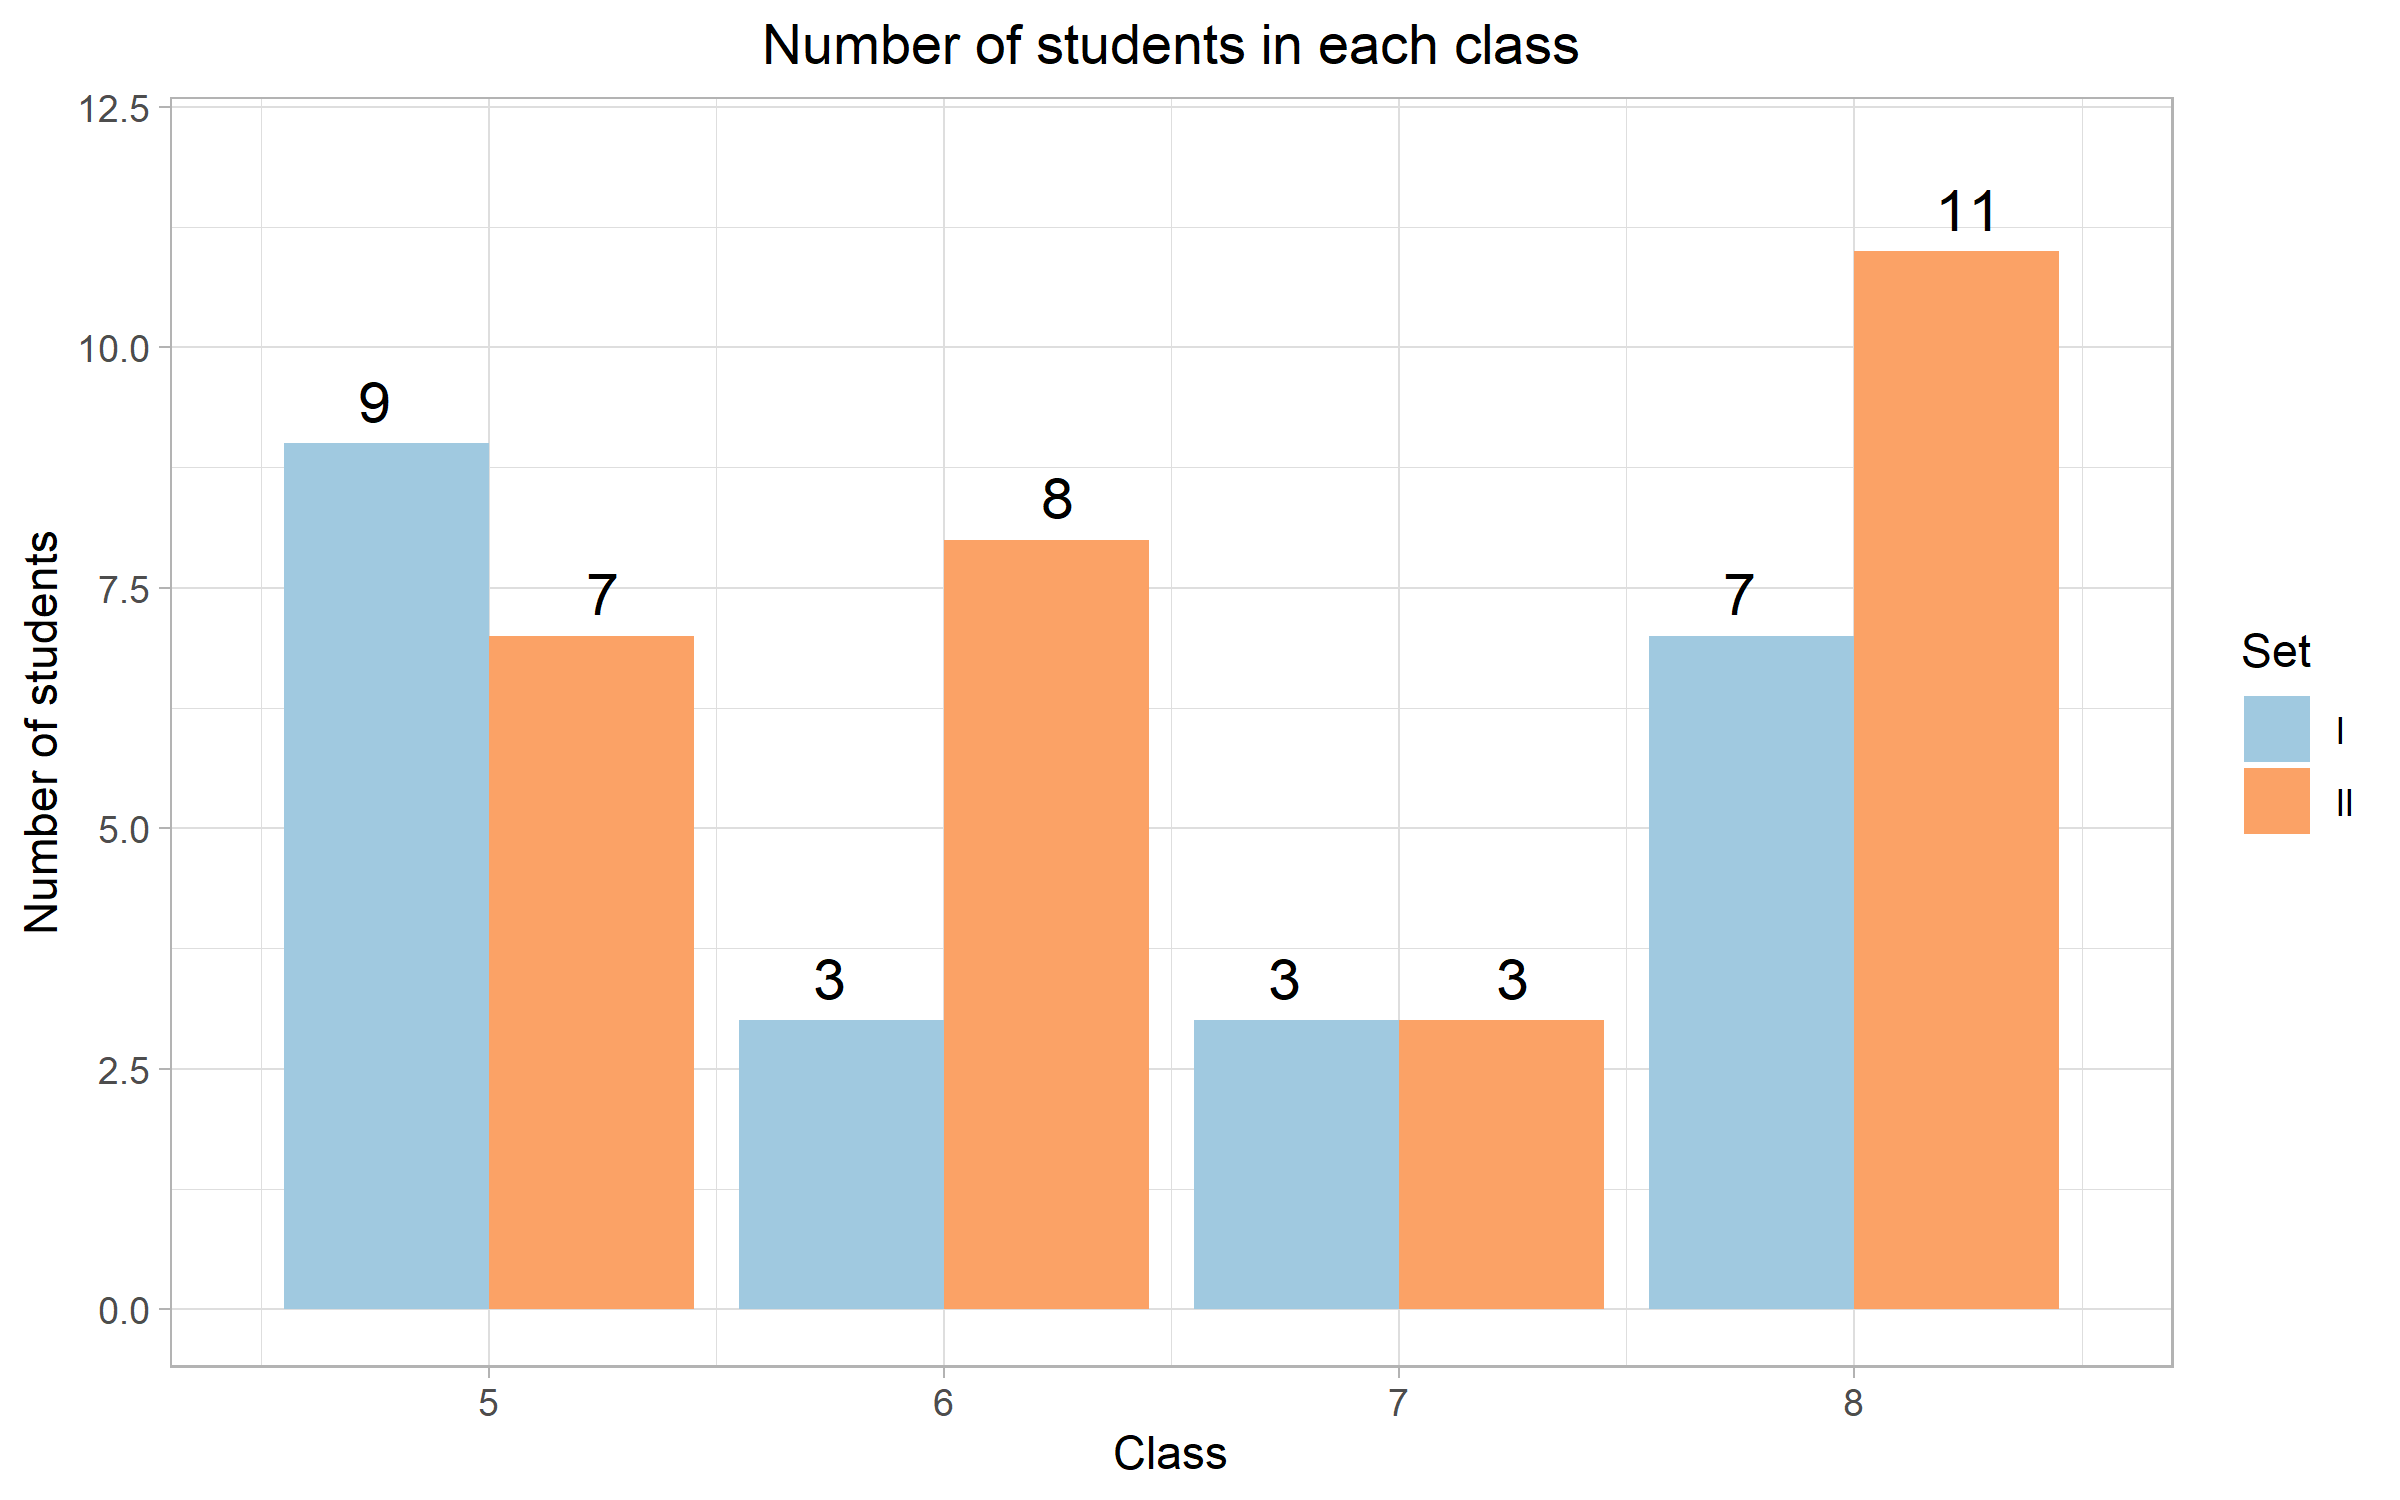
\includegraphics[width=0.7\textwidth]{Number_of_students.png}
		\caption{The number of students in each class, broken down by the version of the test they were solving.}
		\label{students_in_classes}
	\end{figure}
	
	In Table \ref{tab:item_param_gr} are presented minimums, maximums, means and standard deviations of mentioned before parameters for two separate groups of examinees (who solved two different versions of the test). Minimum and maximum values of guessing parameters for both groups are equal to 0 and 1, respectively, but greater differences between the parameter values are observed for the first version. The slipping parameters range from 0 to 0.41 for the version I and from 0 to 0.66 for version II. Looking especially at the standard deviation, it can be seen that the opposite situation is true -- greater differences between the slipping parameter values are observed for the second version. The results obtained for item easiness parameter, where mean is equal to 0.71 and 0.70 respectively, confirm these assumptions. The most surprising for both test versions were the results obtained for the item discrimination parameters, especially the minimum, which is equal to -0.11 and -0.66. Such a low value of the item discrimination parameter is caused by the high guessing parameters (equal 1). The item discrimination parameters in such cases can be interpreted as equal 0, which means that for this item it is impossible to separate examinees possessing relevant skills and those who do not. Mean of the $\delta_1$ is equal to 0.41 and 0.43 for the first and the second version of the test respectively, thus the items, in~general, do not separate the examinees well in both cases.
	
	\begin{table}[H]
		\centering
		\begin{tabular}{l r r r r c r r r r} 
			\hline
			{\rule{0pt}{3ex}} & \multicolumn{4}{c}{Version I} & & \multicolumn{4}{c}{Version II} \\
			Type of characteristic & Min & Max & Mean & SD &  & Min & Max & Mean & SD \\
			\hline
			{\rule{0pt}{3ex}}guessing parameters  & 0.00 & 1.00 & 0.51 & 0.39 &  & 0.00 & 1.00 & 0.48 & 0.28 \\
			slipping parameters & 0.00 & 0.41 & 0.09 & 0.11 &  & 0.00 & 0.66 & 0.08 & 0.15 \\ 
			item discrimination & -0.11 & 1.00 & 0.41 & 0.40 &  & -0.66 & 0.86 & 0.43 & 0.34 \\ 
			item easiness & 0.30 & 0.97 & 0.71 & 0.14 &  & 0.43 & 0.94 & 0.70 & 0.14\\ [0.5ex] 
			\hline
		\end{tabular}
		\caption{The summary of item characteristics for two, separate groups.}
		\label{tab:item_param_gr} 
	\end{table}
	
	Figure \ref{histogram_ans_groups} on page \pageref{histogram_ans_groups} shows the distribution of students' answers to both test versions items. None of the examinees responded to less than 7 problems. Most of the students, 70\% in the first group and 72\% in the second group answered correctly to more than 15 questions. On average, students answered correctly to 15.5 and 16.17 questions in groups I and II, respectively. Such results confirm the assumptions that the test turned out to be quite simple for both study groups.
	
	\begin{figure}[ht]
		\centering
		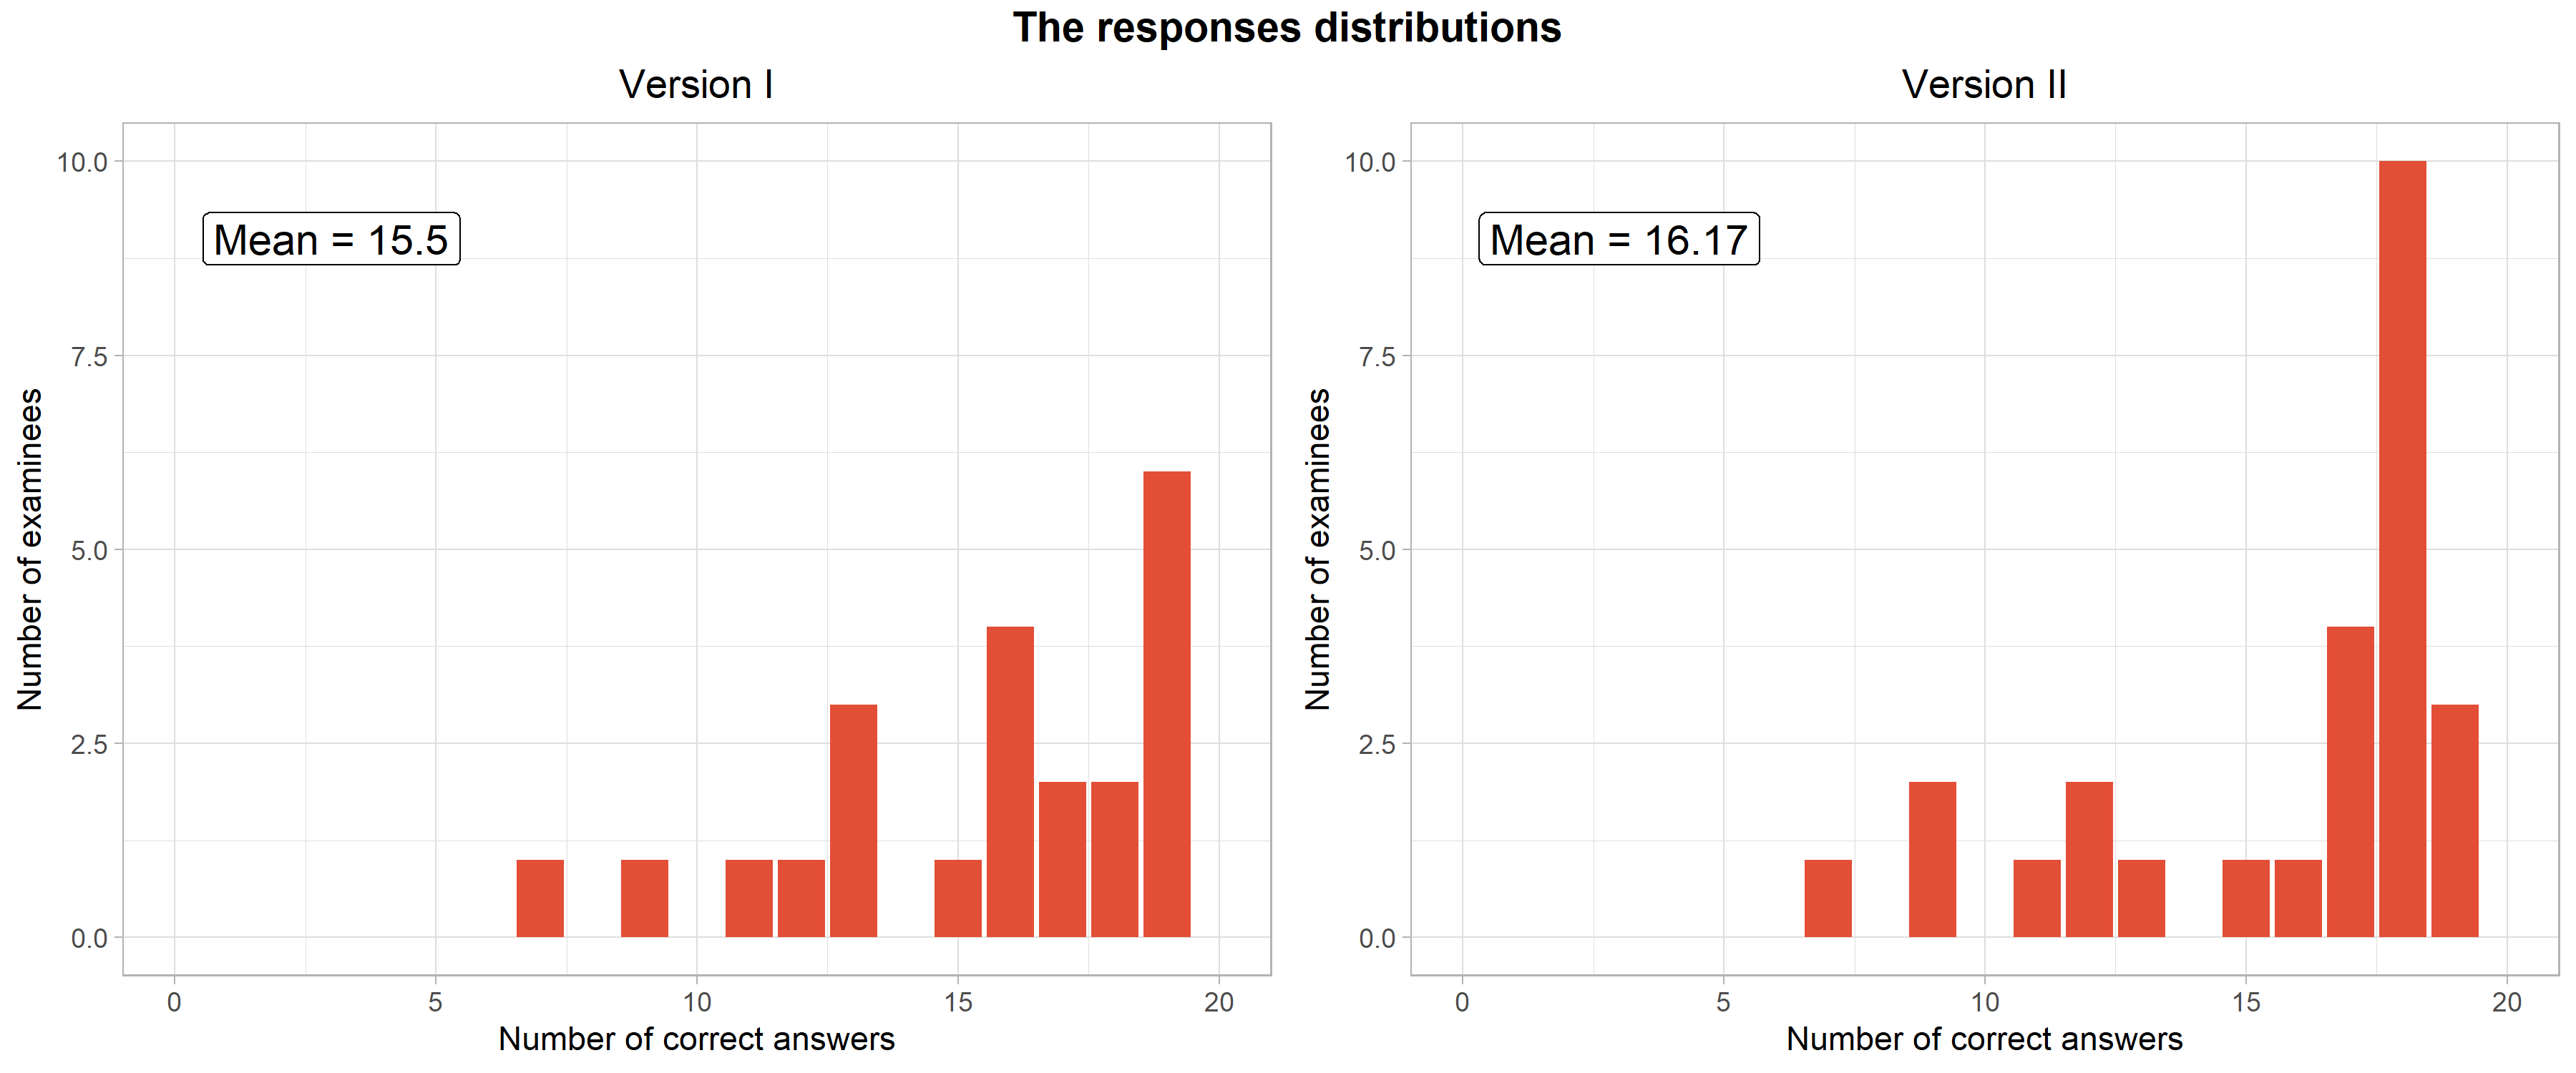
\includegraphics[width=\textwidth]{Responses_distributions.png}
		\caption{Plots of the responses distributions.}
		\label{histogram_ans_groups}
	\end{figure}
	
	Figure \ref{skill_class_dist_groups} on page \pageref{skill_class_dist_groups} presents the skill class distributions for both test versions. Because the test allows checking 8 different attributes, the number of possible skill profiles is equal to $2^8 = 256$ and the value of skill class probability is usually close to 0. What can be observed is that for the first group, three the most likely skill profiles are [11011111] ($P([1,1,0,1,1,1,1,1])=0.32$), [01111111] ($P([0,1,1,1,1,1,1,1])=0.09$), and [11111111] ($P([1,1,1,1,1,1,1,1])=0.18$). Which means that some students had problems with skills $\alpha_1$ (converting a whole number to a fraction) and $\alpha_3$ (simplifying before subtracting). Such a result may be a signal to the teacher that these skills still need to be practiced. For the second group, there is only one significantly probable skills profile [11111111] ($P([1,1,1,1,1,1,1,1])=0.65$). The probability of having at least 7 skills is very high (for the first group it is equal almost 64\% and for the second group almost 68\%). Obtained results suggest that in both study groups the majority of the students mastered the skills necessary to subtract fractions.
	
	\begin{figure}[hb!]
		\centering
		\begin{multicols}{2}
			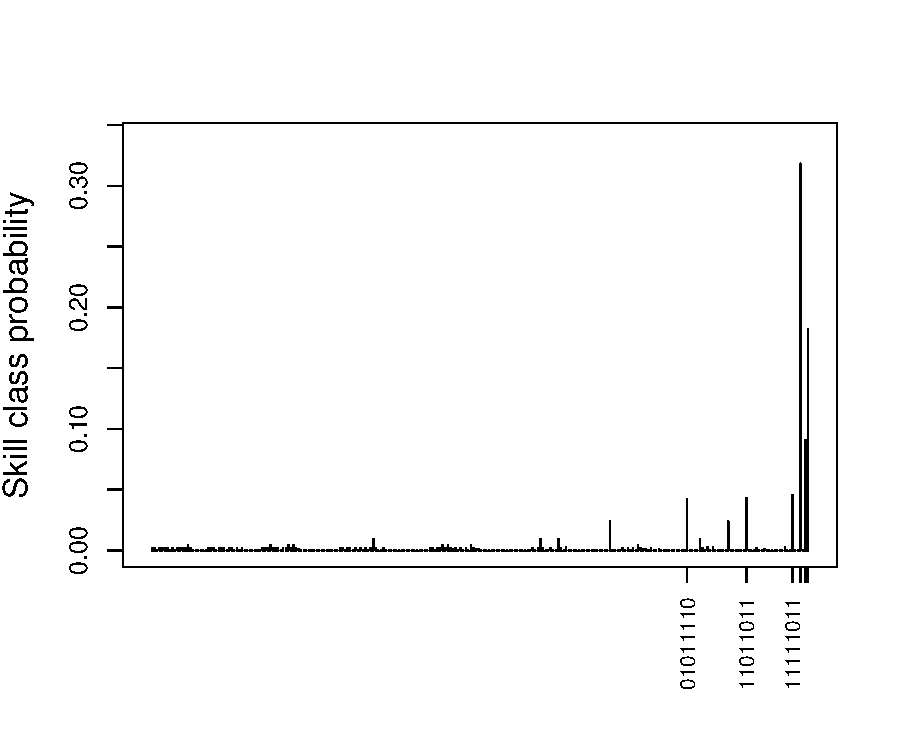
\includegraphics[width=0.5\textwidth]{Skill_class_probability_1.pdf}
			
			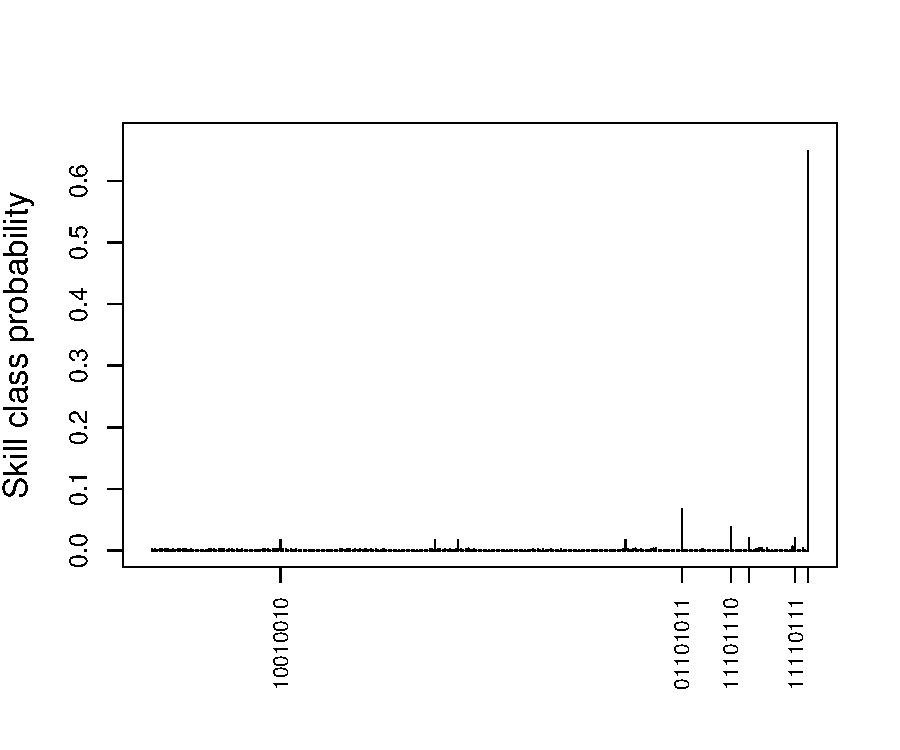
\includegraphics[width=0.5\textwidth]{Skill_class_probability_2.pdf}
		\end{multicols} 
		\caption{Plots of the skill class distributions $P(\alpha_i)$ for two test groups (the version I on the left side and version II on the right side).}\label{skill_class_dist_groups}
	\end{figure}
	
	Figure \ref{skill_possession_groups} on page \pageref{skill_possession_groups} presents two plots of the skill distribution. On average, 77\% of students who solved the first version of the test and 85\% of students who solved the second version, possess all of the skills. For the first group, it can be observed that the~fewest students (only 46\%) possess the $\alpha_3$ skill (simplifying before subtracting), and~the~most (almost 90\%) possess the $\alpha_4$ (finding a common denominator). For the second group, the~skill possessed by the smallest number of students is $\alpha_6$ (borrowing to subtract the second numerator from the first) and the one possessed by the greatest number of examinees is $\alpha_7$ (subtracting numerators). These results are in line with previous observations. The~results themselves are not as bothering as comparing the two groups with each other. On the first sight, it is noticeable that the students taking the second version of the test mostly have all the skills and the most diverse results for the skill mastery probabilities are obtained for the skill $\alpha_3$. Above all, the results obtained for this skill questions the consistency of both versions of the test, so it is important to check if the versions of the tests are comparable.
	
	\begin{figure}[hb!]
		\centering
		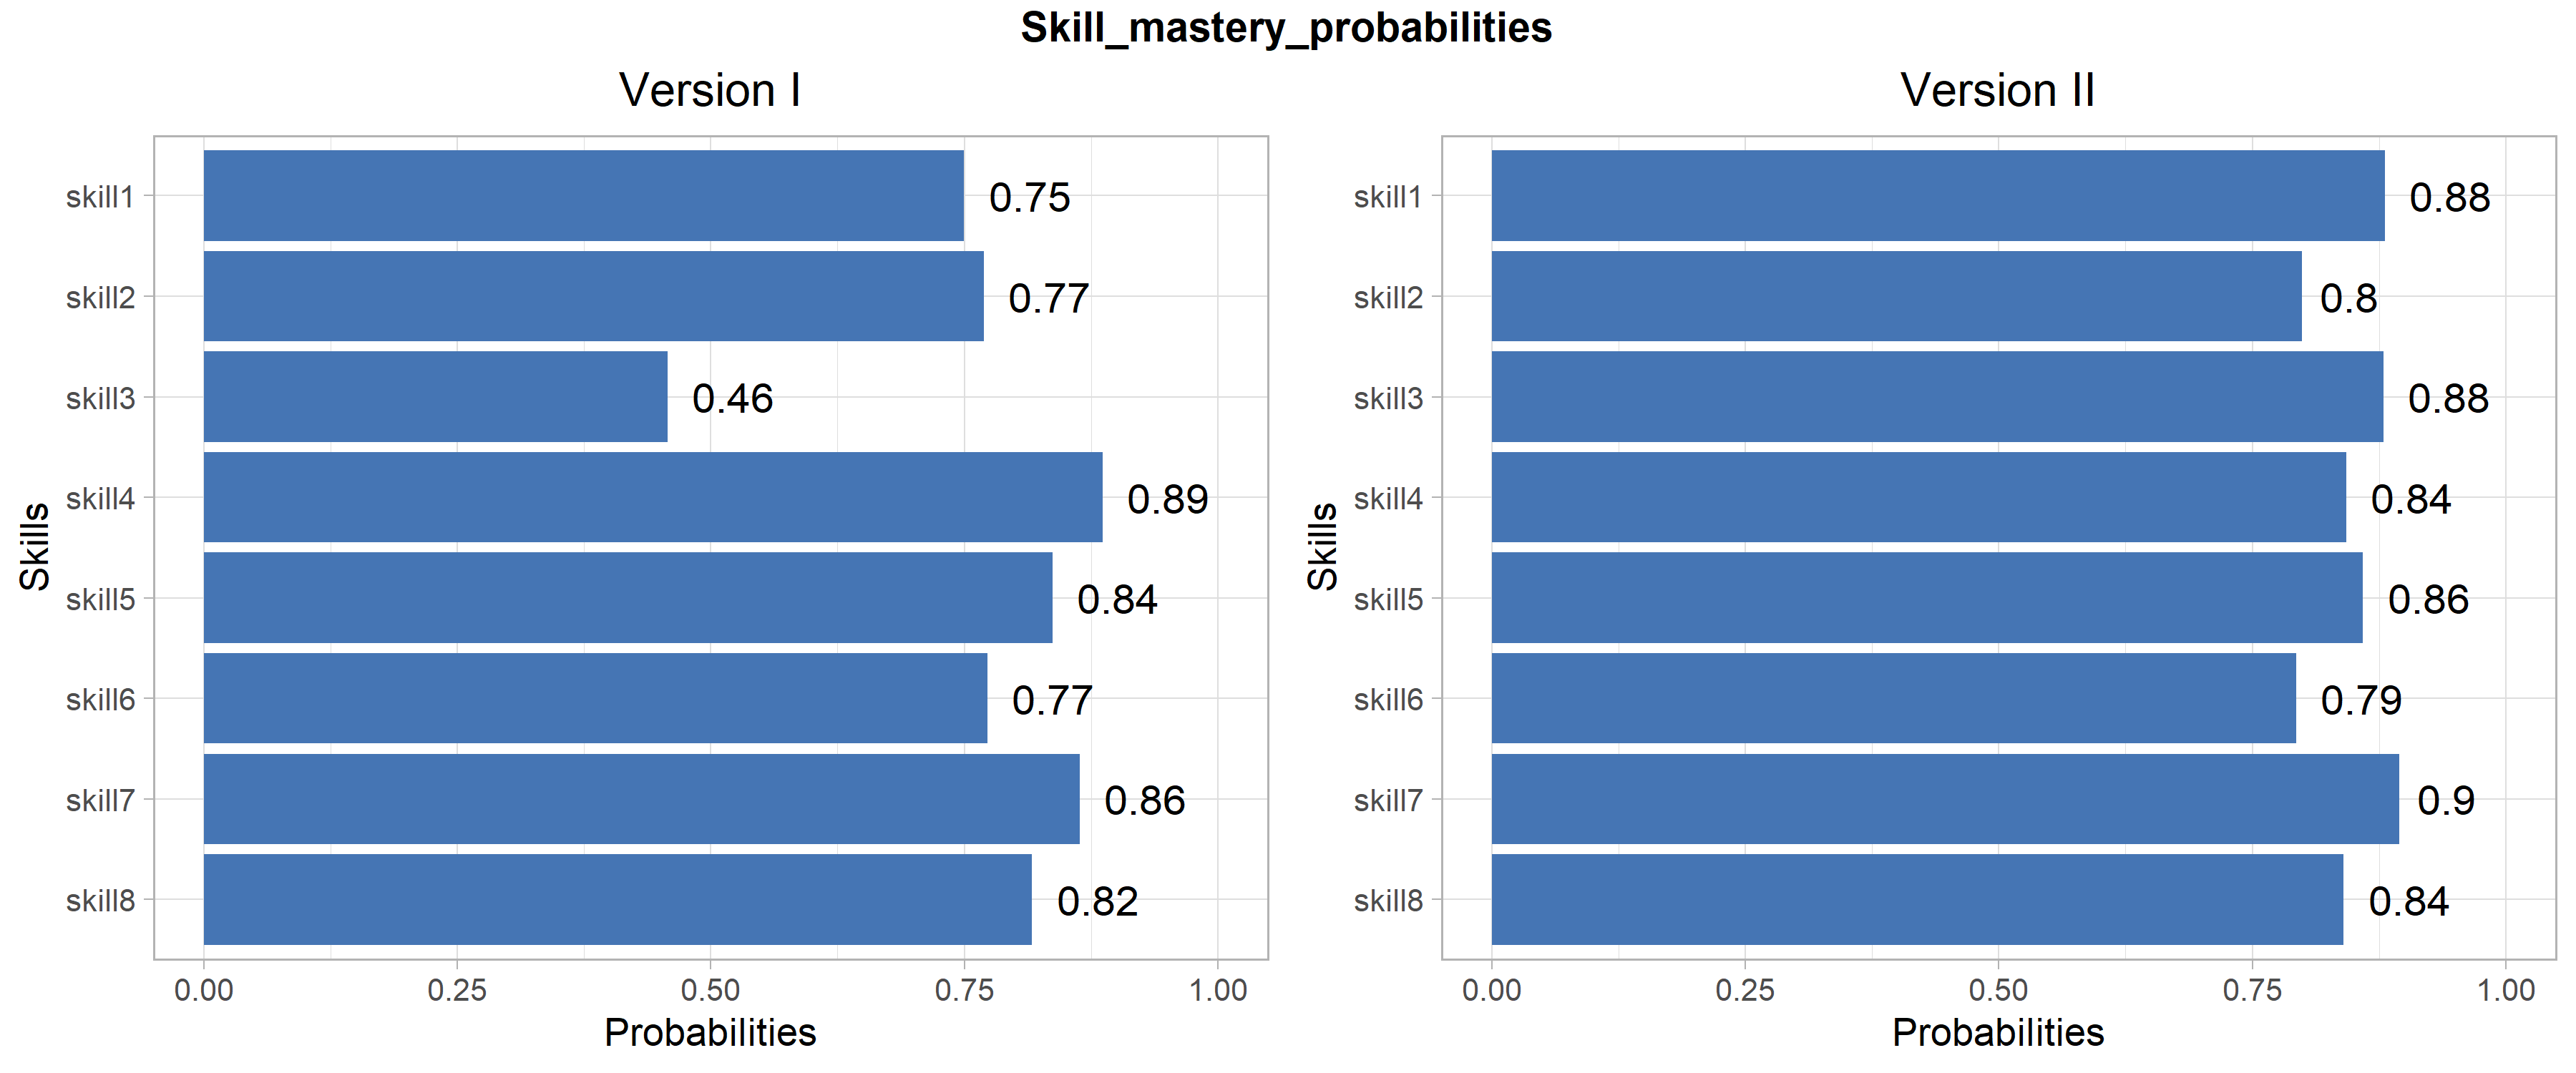
\includegraphics[width=\textwidth]{Skill_mastery_probabilities.png}
		\caption{Plot of the skill distribution $P(\alpha_k)$.}
		\label{skill_possession_groups}
	\end{figure}
	
	To compare the version of the test, two sequences of random variables should be analyzed
	$$ X_1, \ldots, X_8 \sim \mathcal{B}(p_1,22),\ldots,\mathcal{B}(p_8,22) $$
	\noindent and
	$$ Y_1, \ldots, Y_8 \sim \mathcal{B}(q_1,29),\ldots,\mathcal{B}(q_8,29), $$
	where $\mathcal{B}(s,n)$ is the binomial distribution, $s$ is a success probability for each trial and $n$ is a number of trials. In this case, $n$ is equal to the number of students solving each of the test versions (22 and 29 for the first and the second version respectively) and the probabilities $(p_1,\ldots,p_8)$ and $q_1,\ldots,q_8)$ are related to the number of students who possess particular skills $\alpha_1,\ldots,\alpha_8$. The necessary assumption is that the possession of skills is independent. 
	
	Having defined the above expressions, it is possible to perform a two-sample proportion hypothesis tests \cite{proportion_test} and check the following hypotheses
	$$ H_0: p_k = q_k \qquad \text{and} \qquad H_1: p_k \neq q_k.$$
	
	Such hypotheses should be tested for each of the skills $\alpha_{k}$, but based on the independence of the skills, it is possible to apply the Bonferroni correction, which is a statistical tool to counteract the problem of multiple comparisons, by reducing the nominal significance level of each set of related tests in direct proportion to their total number \cite{bonferroni}. Thanks to this, the proportion test will be a test of all 8 skills. Assuming the significance level for the entire test is to be $\gamma = 0.05$, the test for each skill will have a significance level of $\gamma_k = \frac{0.05}{8} = 0.00625$. 
	
	The \texttt{prop.test()} function from the \texttt{stats} library was used to carry out the test\footnote{Source: https://www.rdocumentation.org/packages/stats/versions/3.6.2/topics/prop.test (access: VIII 2020)}. The function arguments are a vector of counts of trials $n$ (22 for the first test version and 29 for the second in this case) and a vector of counts of successes $x$ ($x_1$ for the first test version and $x_2$ for the second one). Table \ref{tab:p_values_groups_comparison} presents percentages of successes for the first ($x_1/22$) and the second ($x_2/29$) test versions, and obtained in the test of proportion $p$-values for the each skill.
	
	\begin{table}[H]
		\centering
		\begin{tabular}{c c c c c c c c c} 
			\hline
			{\rule{0pt}{3ex}} & \multicolumn{8}{c}{Skill} \\
			& $\alpha_1$ & $\alpha_2$ & $\alpha_3$ &  $\alpha_4$ & $\alpha_5$ & $\alpha_6$ & $\alpha_7$ & $\alpha_8$ \\
			\hline
			{\rule{0pt}{3ex}}$x_1/22$ & 0.73 & 0.82 & 0.50 & 0.86 & 0.86 & 0.68 & 0.86 & 0.82 \\
			$x_2/29$ & 0.66 & 0.79 & 0.72 & 0.83 & 0.86 & 0.76 & 0.93 & 0.90 \\
			$p$-value & 0.8065 & 1.0000 & 0.1779 & 1.0000 & 1.0000 & 0.7703 & 0.7442 & 0.6931 \\ [0.5ex] 
			\hline
		\end{tabular}
		\caption{The vectors of counts of successes and $p$-values for each skill $\alpha_{k}$.}
		\label{tab:p_values_groups_comparison} 
	\end{table}
	
	None of the $p$-values is less than the significance level $\gamma_k = 0.00625$, which means that there are no grounds to reject the null hypothesis in any of the cases. It can be concluded that the groups solving the tests performed comparably, and knowing that the students were assigned to the tests randomly, it can be concluded that the tests were also comparable.
	
	\subsubsection{Analysis of all students}
	
	Knowing that both versions of the test are comparable, it is possible to repeat the previous analysis for the whole group of examinees. Table \ref{tab:item_param} on page \pageref{tab:item_param} presents estimated guessing $g_j$ and slipping $s_j$ parameters, item easiness $\delta_{2,j}$, item discrimination $\delta_{1,j}$ and item $p$-values, which are the percentage of students who responded the item correctly. Minimum and maximum values for guessing parameter were obtained once and they are equal to 0 and 1 respectively. The slipping parameters range from 0 to 0.451, but the value 0 occurred 6 times. Looking at the p-values: the least, because only 51\%, of students answered the item 20, the most, 94.1\%, of the students solved the item 16. 
	
	It is worth focusing on the item easiness and the item discrimination parameters. The~analysis of these two parameters may improve the test. If it turns out that the test contains a difficult item that does not discriminate against the group of students, then it~makes sense to remove it. Such a procedure will not adversely affect the quality of the test, and the reduced number of items will be beneficial for both respondents and teachers. For the item easiness parameter, the mean is equal to 0.72, what confirm assumptions about the difficulty of the test. The most difficult items are the 9th (the item easiness value equal to 0.42) and 20th (0.458). Two the easiest items are the 19th (0.914) and 16th (0.902). Such results coincide with the $p$-values obtained for these items. Mean of the item discrimination parameter $\delta_1$ is equal to 0.39, thus the items, in general, do not separate the examinees well. The two items, that do best to separate students possessing relevant skills from those who do not, are the 1st (0.859) and 9th (0.840) items. The item discrimination minimum is equal to -0.45 and it was achieved for the 6th item. For this item, it is impossible to separate examinees possessing relevant skills and those who do not. Another item that also poorly demarcates the students' skills is the 18th item (0.079). The most difficult items discriminate well, however, perhaps it is worth considering removing from the test the 19th item with one of the lowest item discrimination values, because the item was solved correctly by over 90\% of all students, so it does not significantly contribute to the analysis of the test results.
	
	\begin{table}[h]
		\centering
		\begin{tabular}{l c c c c c} 
			\hline
			{\rule{0pt}{3ex}} & \multicolumn{5}{c}{Parameters}\\
			Item & $g_j$ & $s_j$ & $p_j$ & $\delta_{2,j}$ & $\delta_{1,j}$ \\
			\hline
			{\rule{0pt}{3ex}}1 & 0.116 & 0.025 & 0.706 & 0.546 & \textbf{0.859} \\
			2 & 0.586 & 0.000 & 0.922 & 0.793 & 0.414 \\ 
			3 & 0.338 & 0.087 & 0.804 & 0.626 & 0.575 \\ 
			4 & 0.708 & 0.059 & 0.843 & 0.825 & 0.233 \\
			5 & 0.510 & 0.000 & 0.824 & 0.755 & 0.490 \\
			6 & 1.000 & 0.451 & 0.627 & 0.775 & \textbf{-0.451} \\
			7 & 0.598 & 0.267 & 0.686 & 0.666 & 0.135 \\
			8 & 0.688 & 0.029 & 0.922 & 0.830 & 0.283 \\
			9 & 0.000 & 0.160 & 0.588 & \textbf{0.420} & 0.840 \\
			10 & 0.575 & 0.036 & 0.824 & 0.770 & 0.389 \\
			11 & 0.539 & 0.055 & 0.824 & 0.742 & 0.406 \\
			12 & 0.744 & 0.000 & 0.922 & 0.872 & 0.256 \\
			13 & 0.437 & 0.142 & 0.725 & 0.648 & 0.421 \\
			14 & 0.150 & 0.056 & 0.706 & 0.547 & 0.794 \\
			15 & 0.356 & 0.020 & 0.824 & 0.668 & 0.624 \\
			16 & 0.804 & 0.000 & \textbf{0.941} & 0.902 & 0.196 \\
			17 & 0.608 & 0.000 & 0.882 & 0.804 & 0.392 \\
			18 & 0.831 & 0.090 & 0.882 & 0.871 & 0.079 \\
			19 & 0.828 & 0.000 & 0.922 & \textbf{0.914} & 0.172 \\
			20 & 0.130 & 0.215 & \textbf{0.510} & 0.458 & 0.655\\ [0.5ex] 
			\hline
		\end{tabular}
		\caption{The summary of item characteristics containing guessing $g_j$ and slipping $s_j$ parameters, $p$-values, and item easiness $\delta_{2,j}$ and item discrimination $\delta_{1,j}$ parameters.}
		\label{tab:item_param} 
	\end{table}
	
	Figure \ref{histogram_ans} on page \pageref{histogram_ans} shows the distribution of students' answers to the test items. None of the examinees responded to less than 7 problems, more than 58\% of the examinees responded correctly to at least 17 items. Such results confirm the assumptions that the test turned out to be simple for the whole study group. 
	
	\begin{figure}[h!]
		\centering
		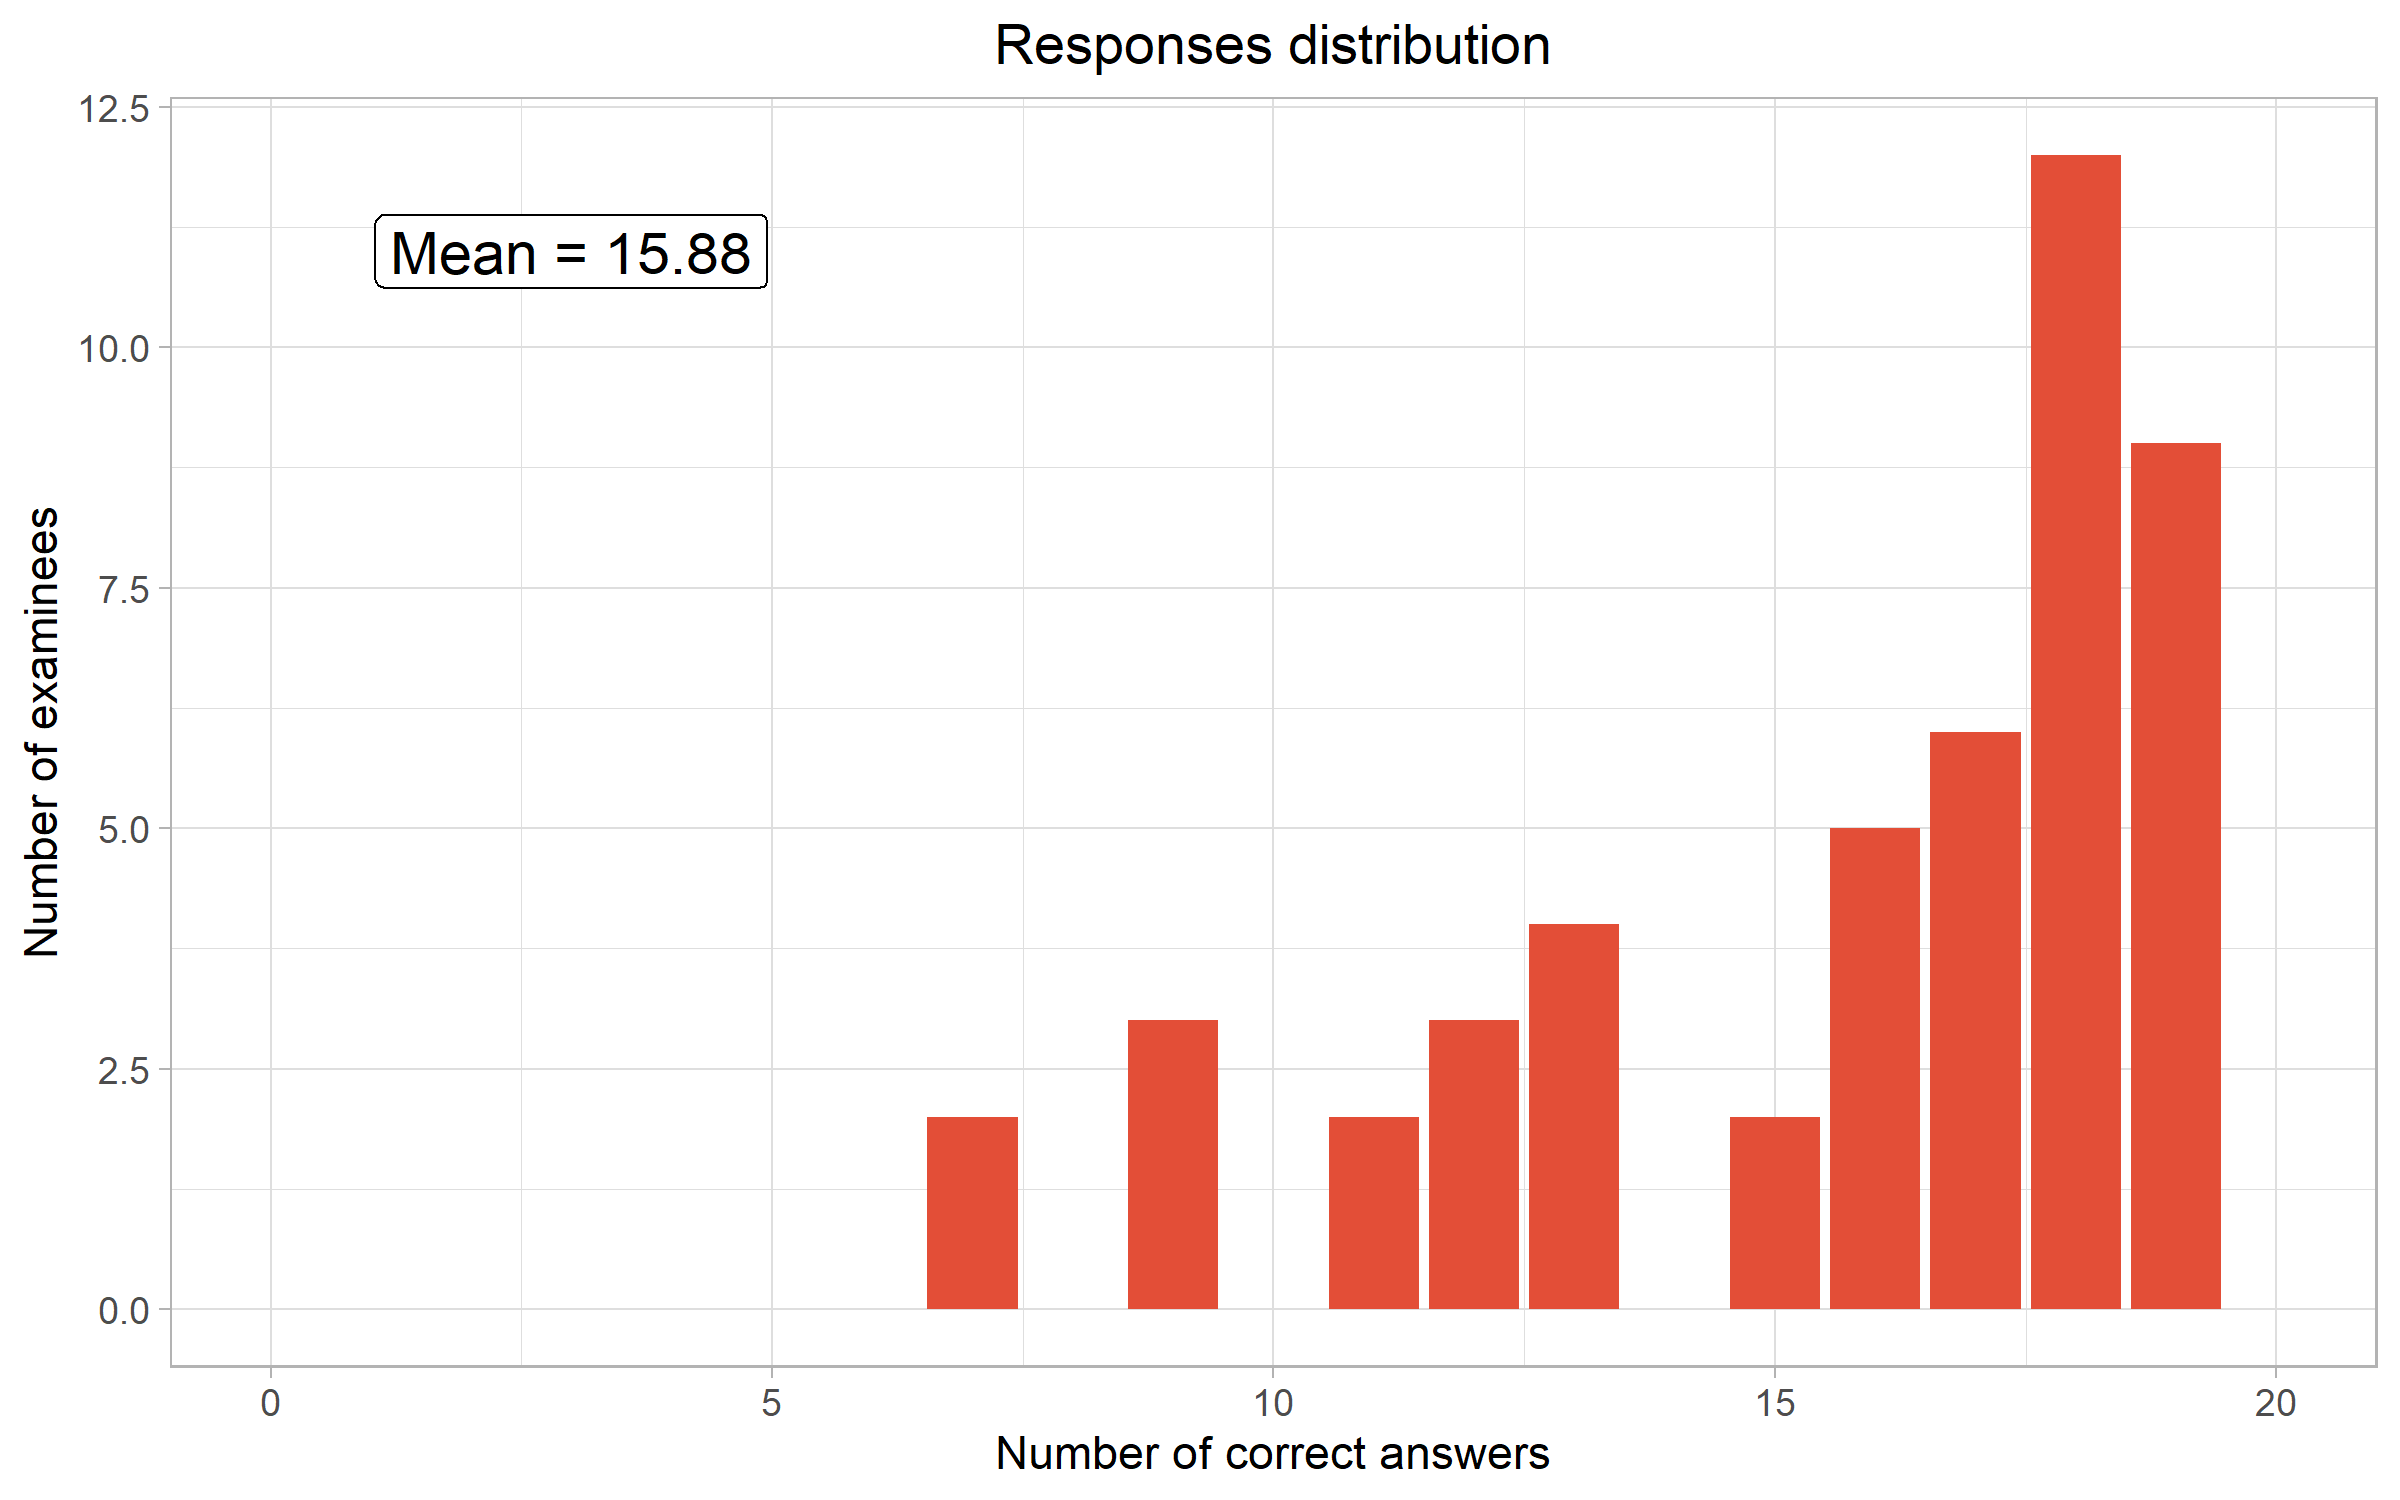
\includegraphics[width=0.7\textwidth]{Responses_distribution.png}
		\caption{Plot of the responses distribution.}
		\label{histogram_ans}
	\end{figure}
	
	Figure \ref{skill_class_dist} on page \pageref{skill_class_dist} presents the skill class distribution. Analysis of the results allows answering the question of what is the proportion of examinees possessing a specific skills' combination. What can be seen is that most examinees possess all skills ($P([1,1,1,1,1,1,1,1])=0.48$). Furthermore, other skill profiles, which probability is higher than or equal to 5\% are $P([1,1,0,1,1,1,1,1])=0.11$ and $P([1,1,1,1,1,0,1,1])=0.05$. In this study group, the probability of having at least 7 skills in bigger than 64\%. It~can be concluded that most students have mastered the skills necessary to solve fraction subtraction problems, but there are still skills that should be practiced more.
	
	\begin{figure}[h!]
		\centering
		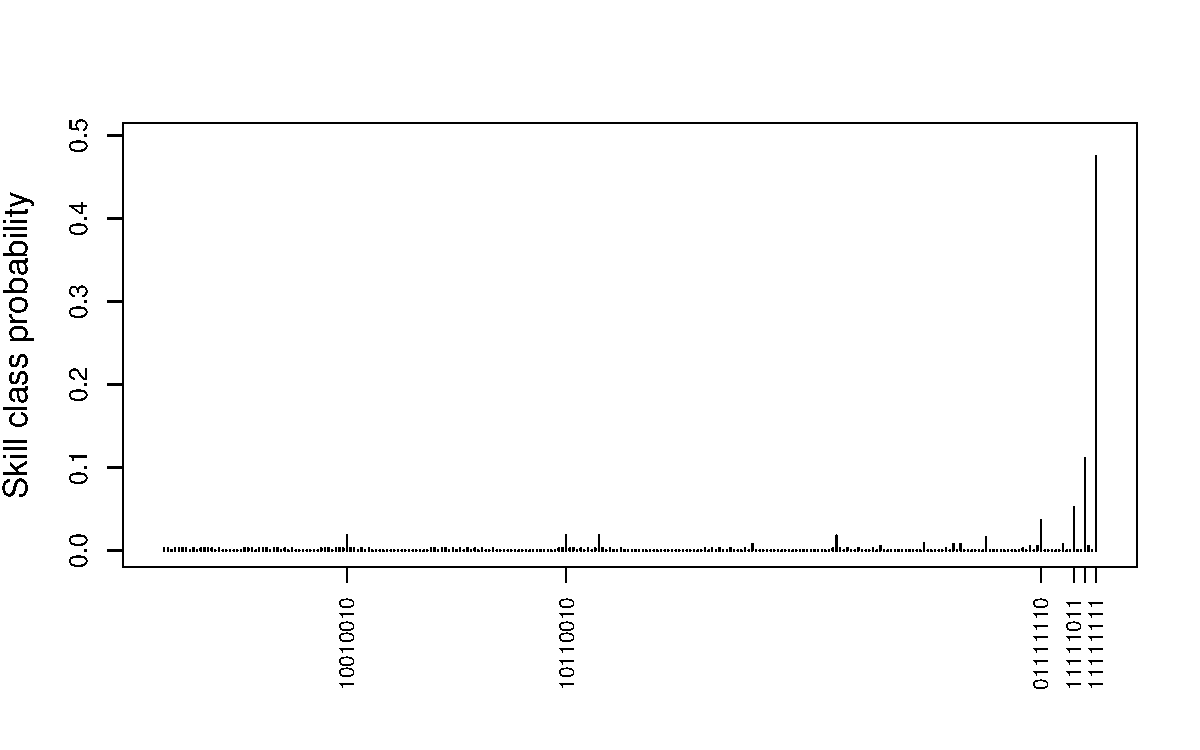
\includegraphics[width=0.7\textwidth]{Skill_class_probability_0.pdf}
		\caption{Plot of the skill class distribution $P(\alpha_i)$.}
		\label{skill_class_dist}
	\end{figure}
	
	Figure \ref{skill_possession} (page \pageref{skill_possession}) presents the skill distribution. On average, 80\% of students possess all of the skills. The fewest students (although as many as 70\%) possess the $\alpha_2$ (separating a whole number from a fraction), and the most (almost 90\%) possess the $\alpha_4$ (finding a~common denominator). The most puzzling fact is that the skill that is possessed by the smallest number of students ($\alpha_2$) does not appear as a skill that is missing in the most popular skill profiles. However, when analyzing the 10 most popular skill profiles, the lack of skill $\alpha_2$ appears in 4 of them. 
	
	\begin{figure}[h!]
		\centering
		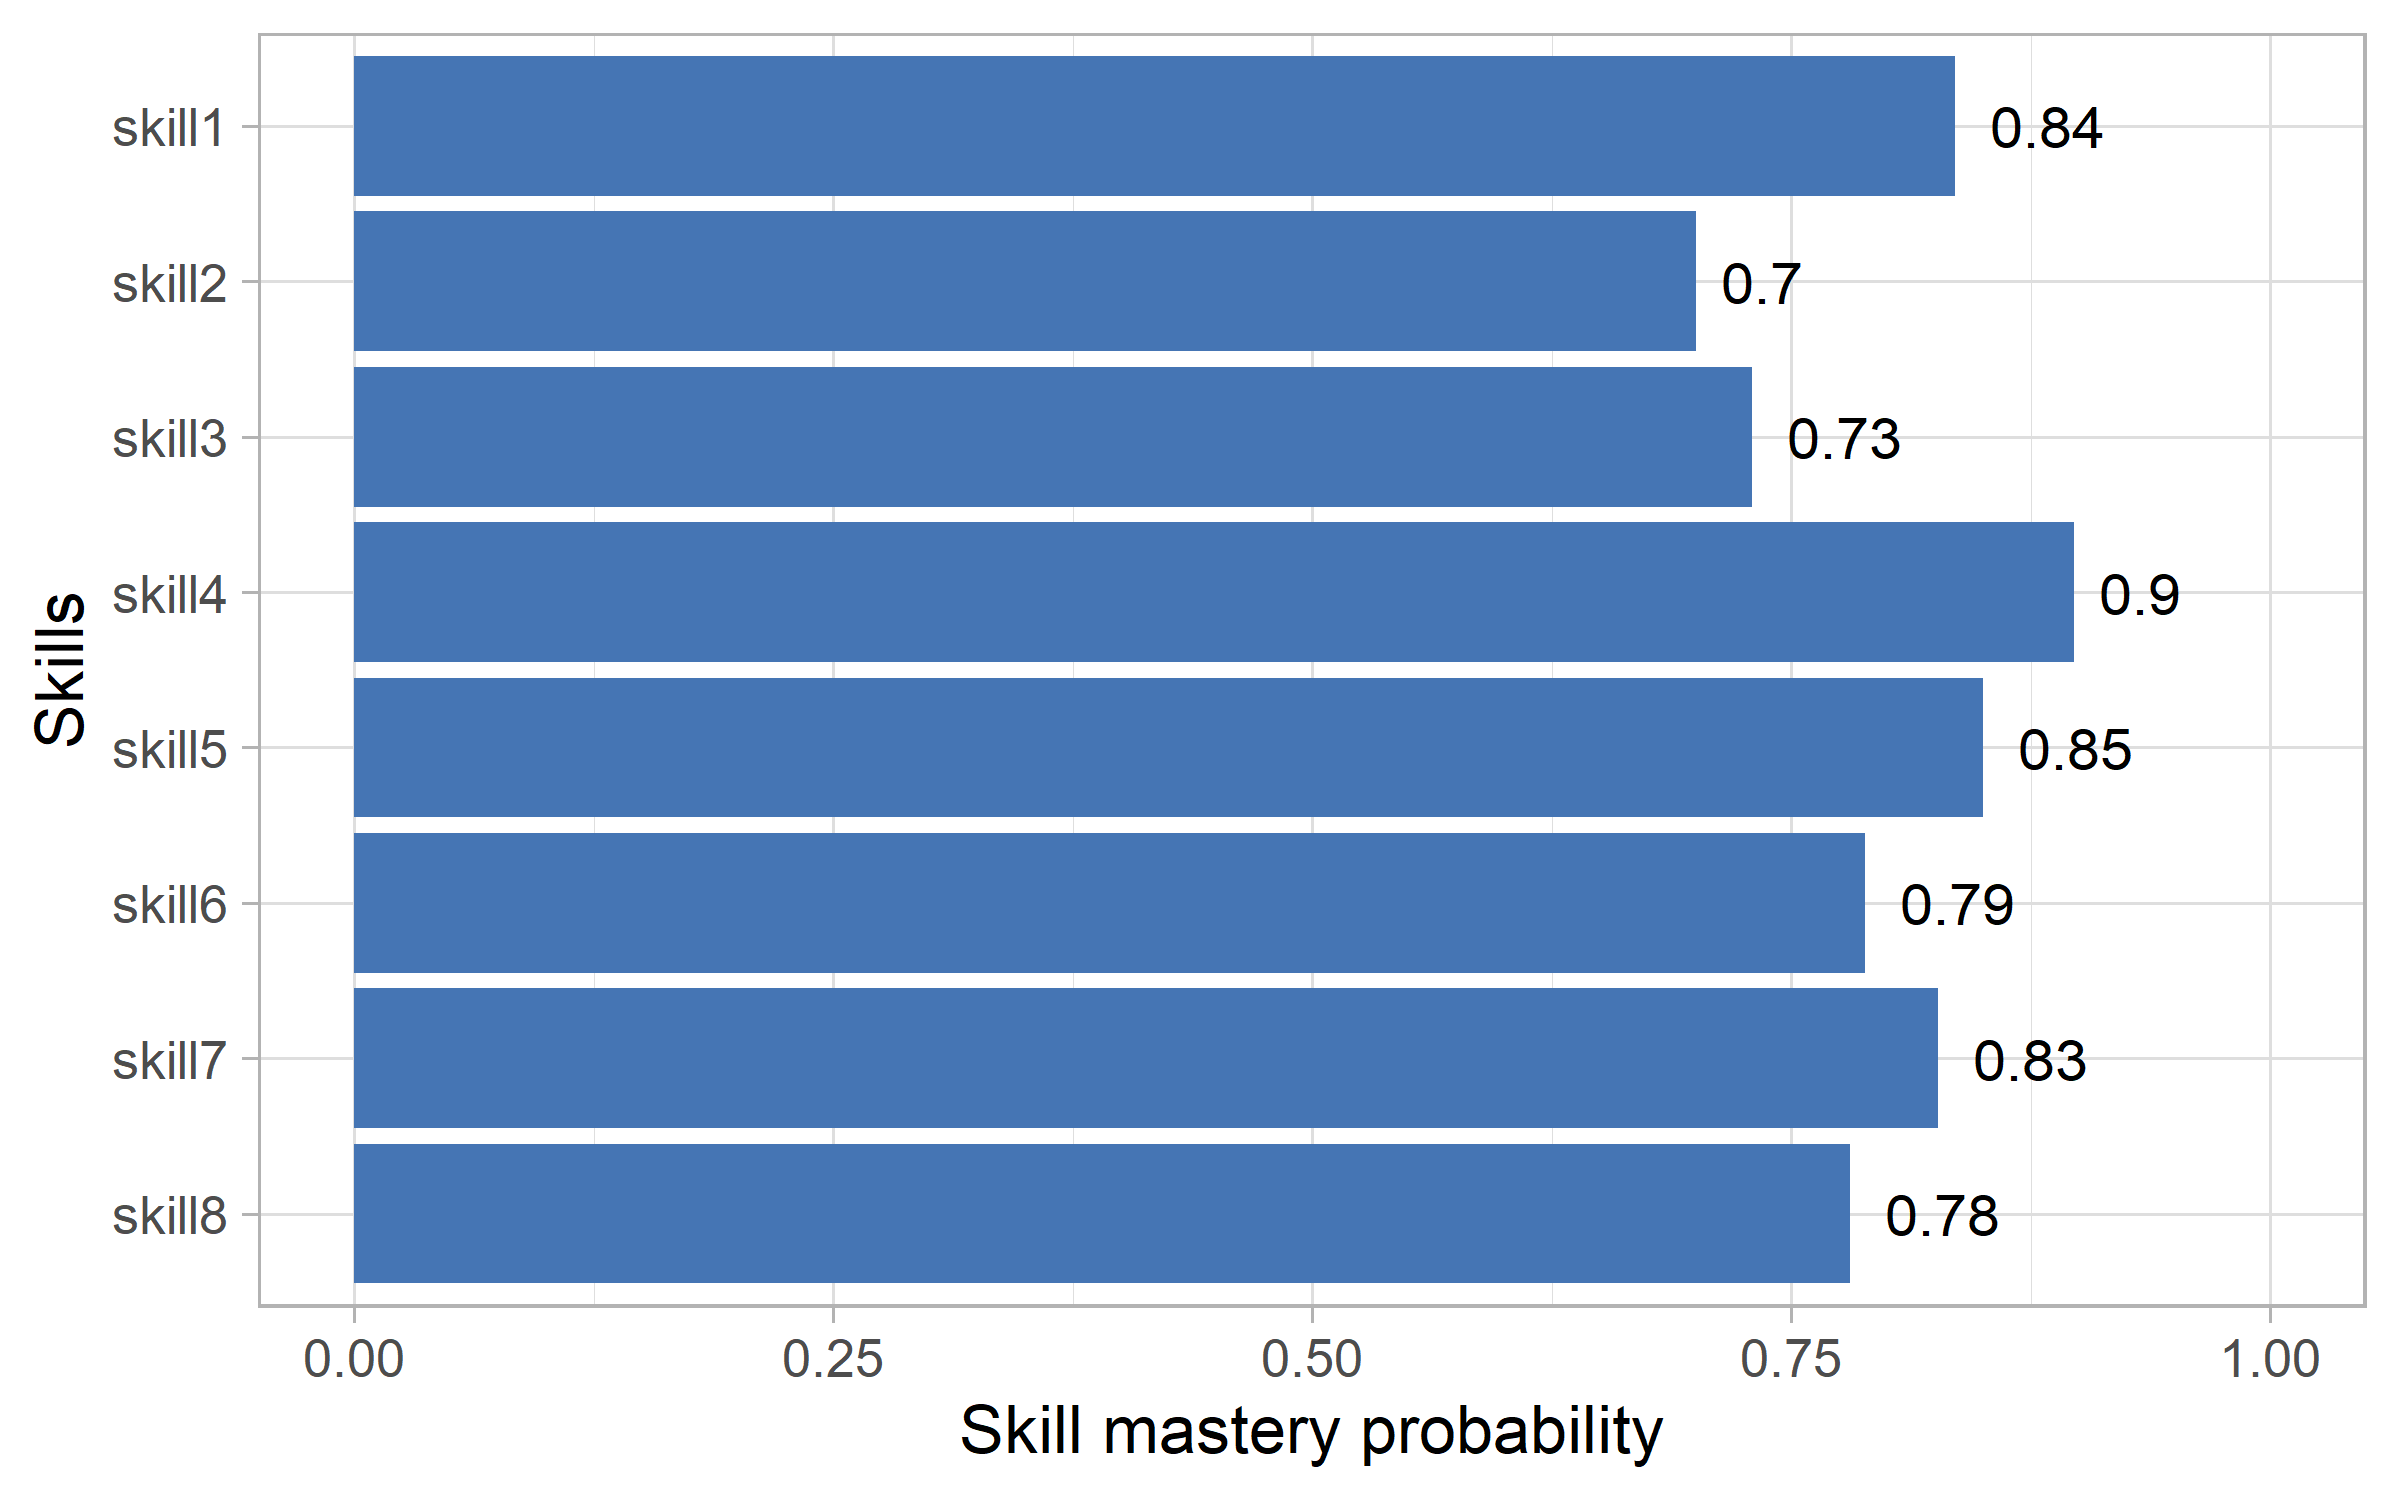
\includegraphics[width=0.7\textwidth]{Skill_mastery_probability.png}
		\caption{Plot of the skill distribution $P(\alpha_k)$.}
		\label{skill_possession}
	\end{figure}
	
	In summary, the test turned out to be simple for a group of 51 examined students. Almost half of them mastered all the skills checked by the test. None of the examinees responded correctly to less than 7 items and item easiness parameter was 71\% on average. Importantly for teachers, the analysis of the test results using Cognitive Diagnosis Models revealed which skills still need to be practiced.
	
	\subsubsection{Analysis of simulated data}
	The previous analysis involved a group of 51 students. Because the group of the examinees was very small, this part will be concerned an additional simulation in which 1000 random responses (with achieved for the real group of students slipping $s$ and guessing $g$ parameters) will be generated with DINA model. Obtained results for the group of respondents and the simulation will be compared.
	
	Figure \ref{histogram_ans_sim} shows the distribution of simulated answers to the test items. The shape of the plot is similar to the density of normal distribution and it is completely different than for the real data. Only 9\% of the simulated responses are correct for more than 15 items, over 37\% of the simulated respondents answered correctly to 9,10 or 11 items. On average, the simulated student answered correctly for 12.09 items.
	
	\begin{figure}[h!]
		\centering
		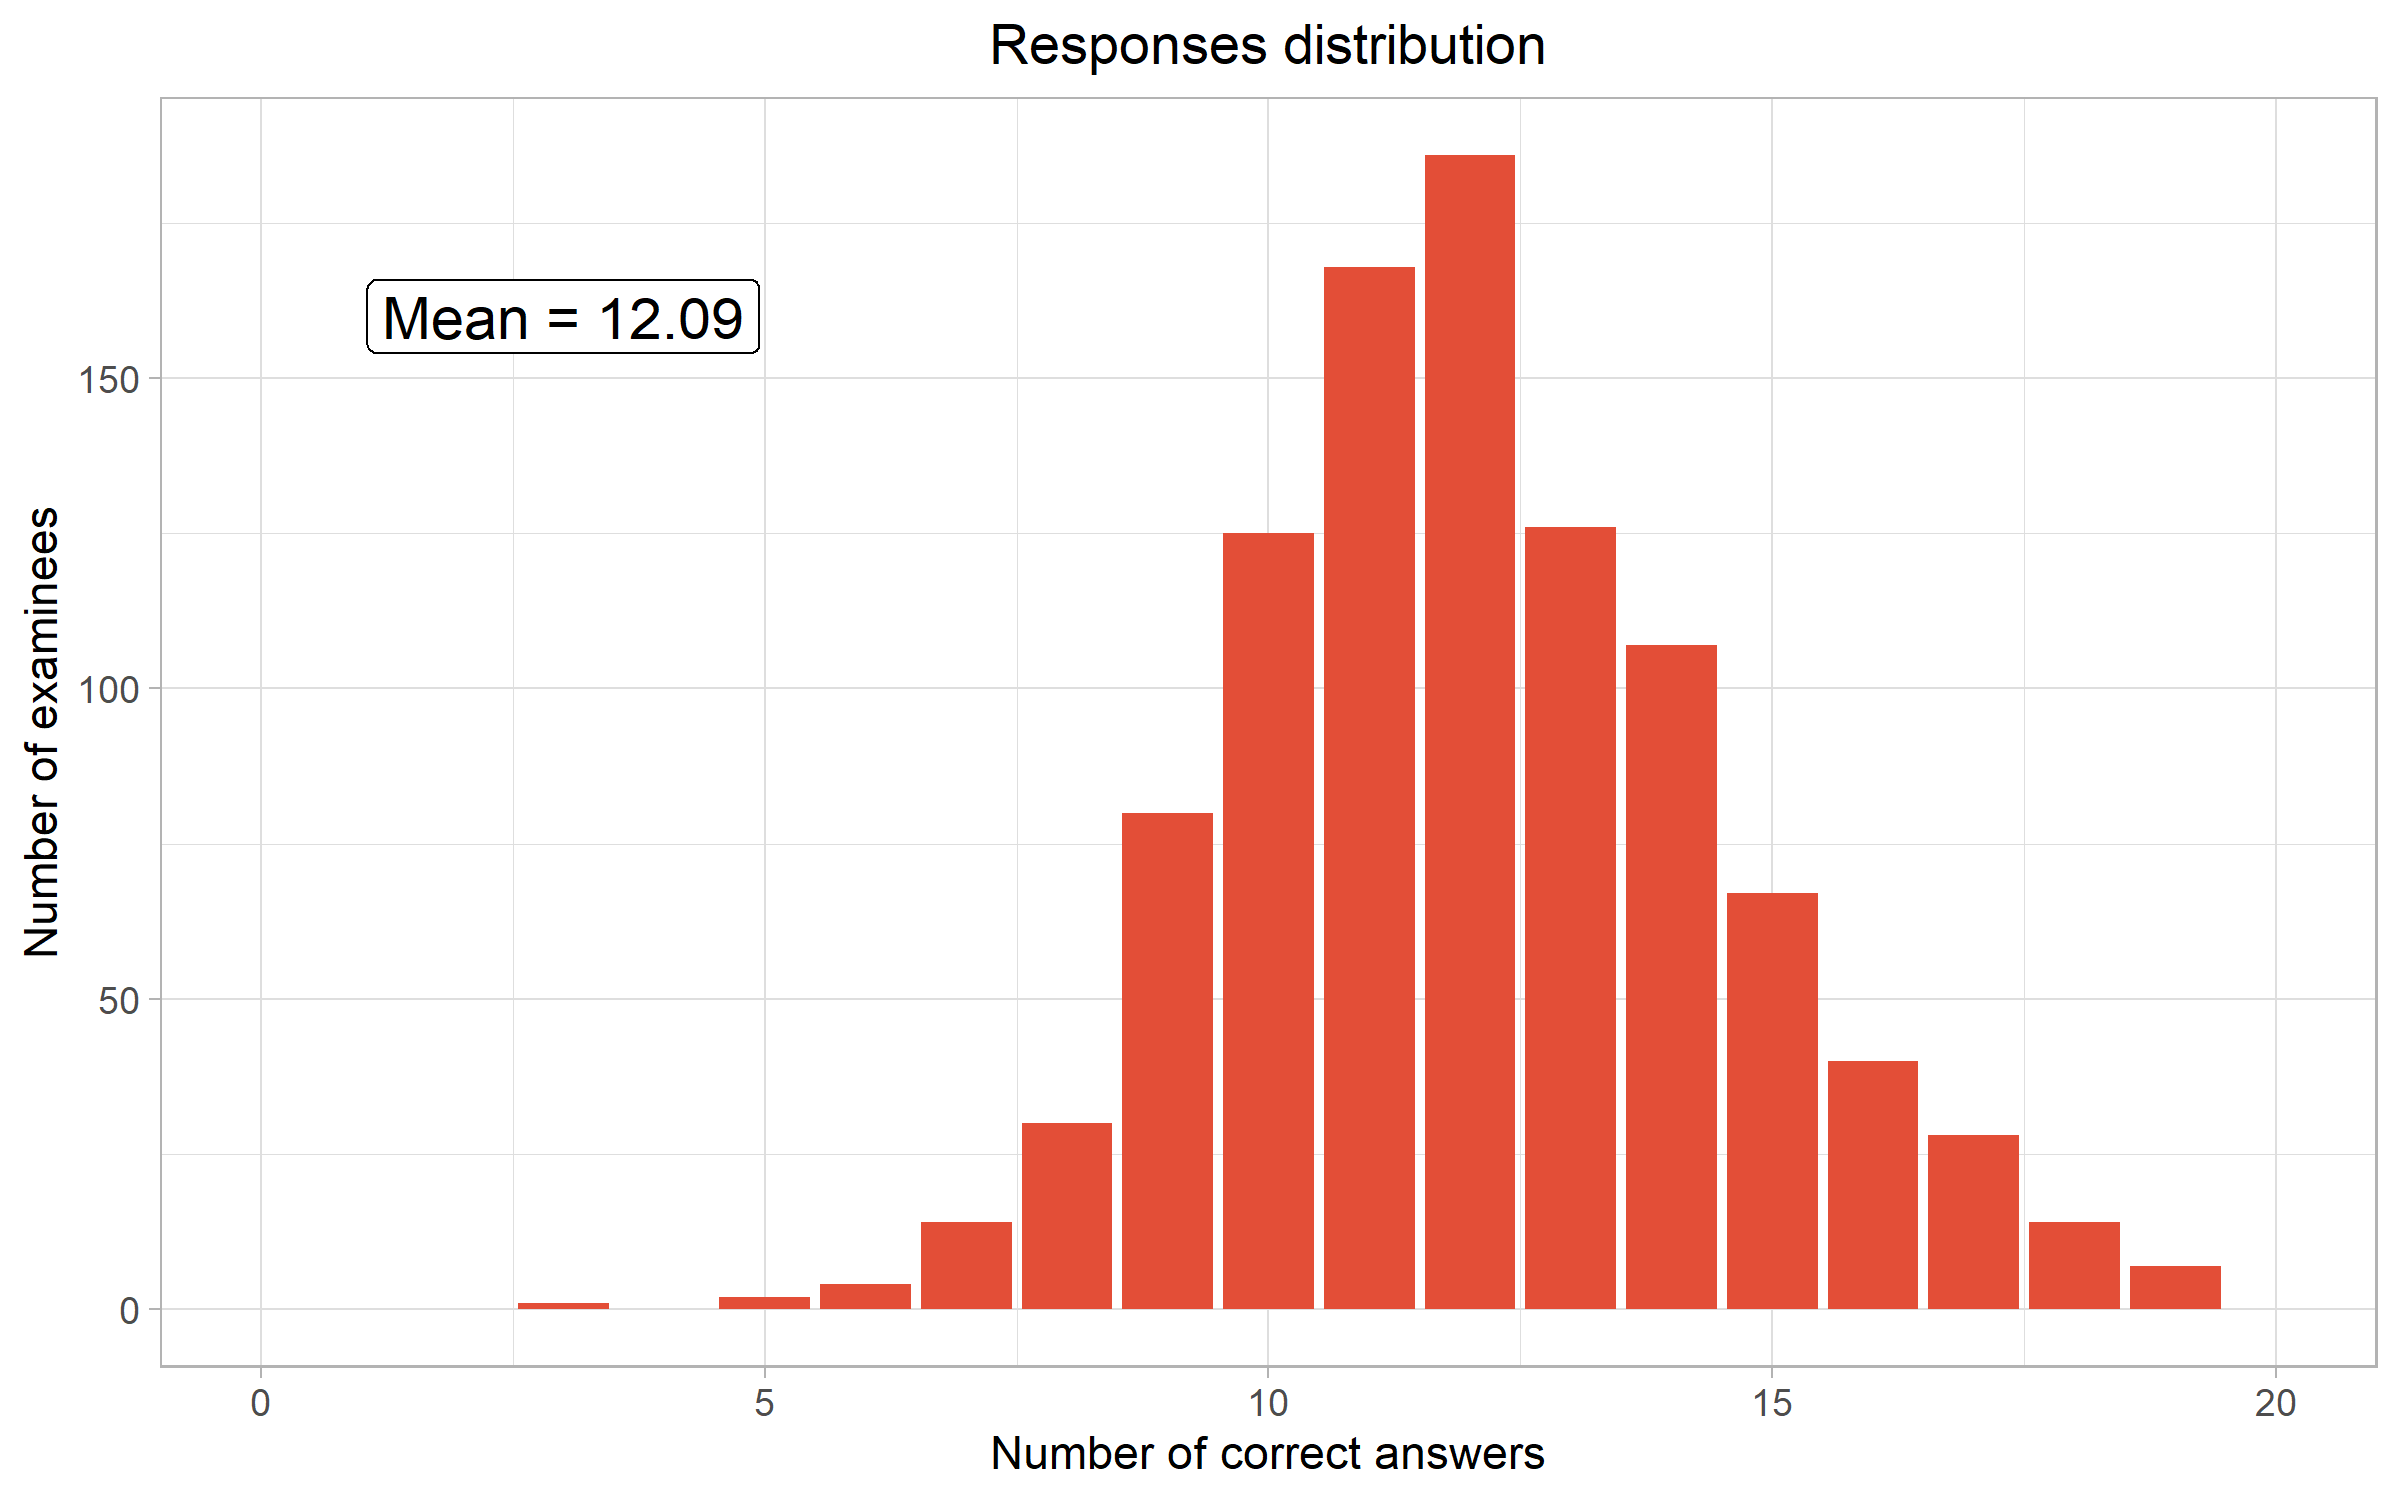
\includegraphics[width=0.7\textwidth]{Responses_sim_distribution.png}
		\caption{Plot of the simulated responses distribution.}
		\label{histogram_ans_sim}
	\end{figure}
	
	Figure \ref{skill_class_dist_sim} on page \pageref{skill_class_dist_sim} presents the skill class distribution. What can be seen, in this case, there is no such distinctive skill profile as previously. None of the probabilities is greater than 2\%. Probabilities higher than 1\% were obtained for the following skill profiles [11001010], [11000011], [01010011], [11100011], [11011010], [11001011], [11000111], [01110011], [01011110], and [11100111]. Probability of having a skill profile with more than 7 skills is very low and it equals 4\%.
	
	\begin{figure}[h!]
		\centering
		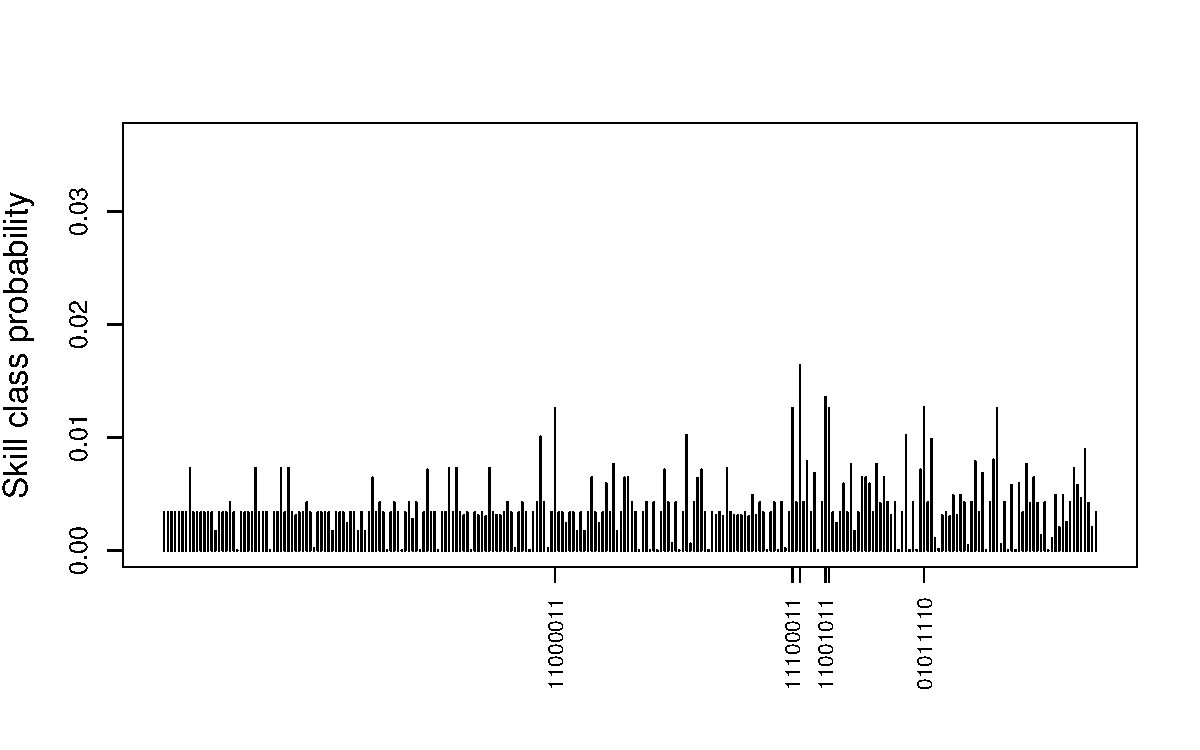
\includegraphics[width=0.7\textwidth]{Skill_class_probability_sim.pdf}
		\caption{Plot of the skill class distribution $P(\alpha_i)$.}
		\label{skill_class_dist_sim}
	\end{figure}
	
	Figure \ref{skill_possession_sim} presents the skill distribution. The resulting plot is significantly different from the plot for the real data. On first sight, it is noticeable that the skill mastery probability is lower. On average, 52\% of simulated students possess all of the skills. The fewest students (48\%) possess the $\alpha_3$ (simplifying before subtracting), and the most (over 58\%) possess the $\alpha_8$ (reducing answers to the simplest form). 
	
	\begin{figure}[h!]
		\centering
		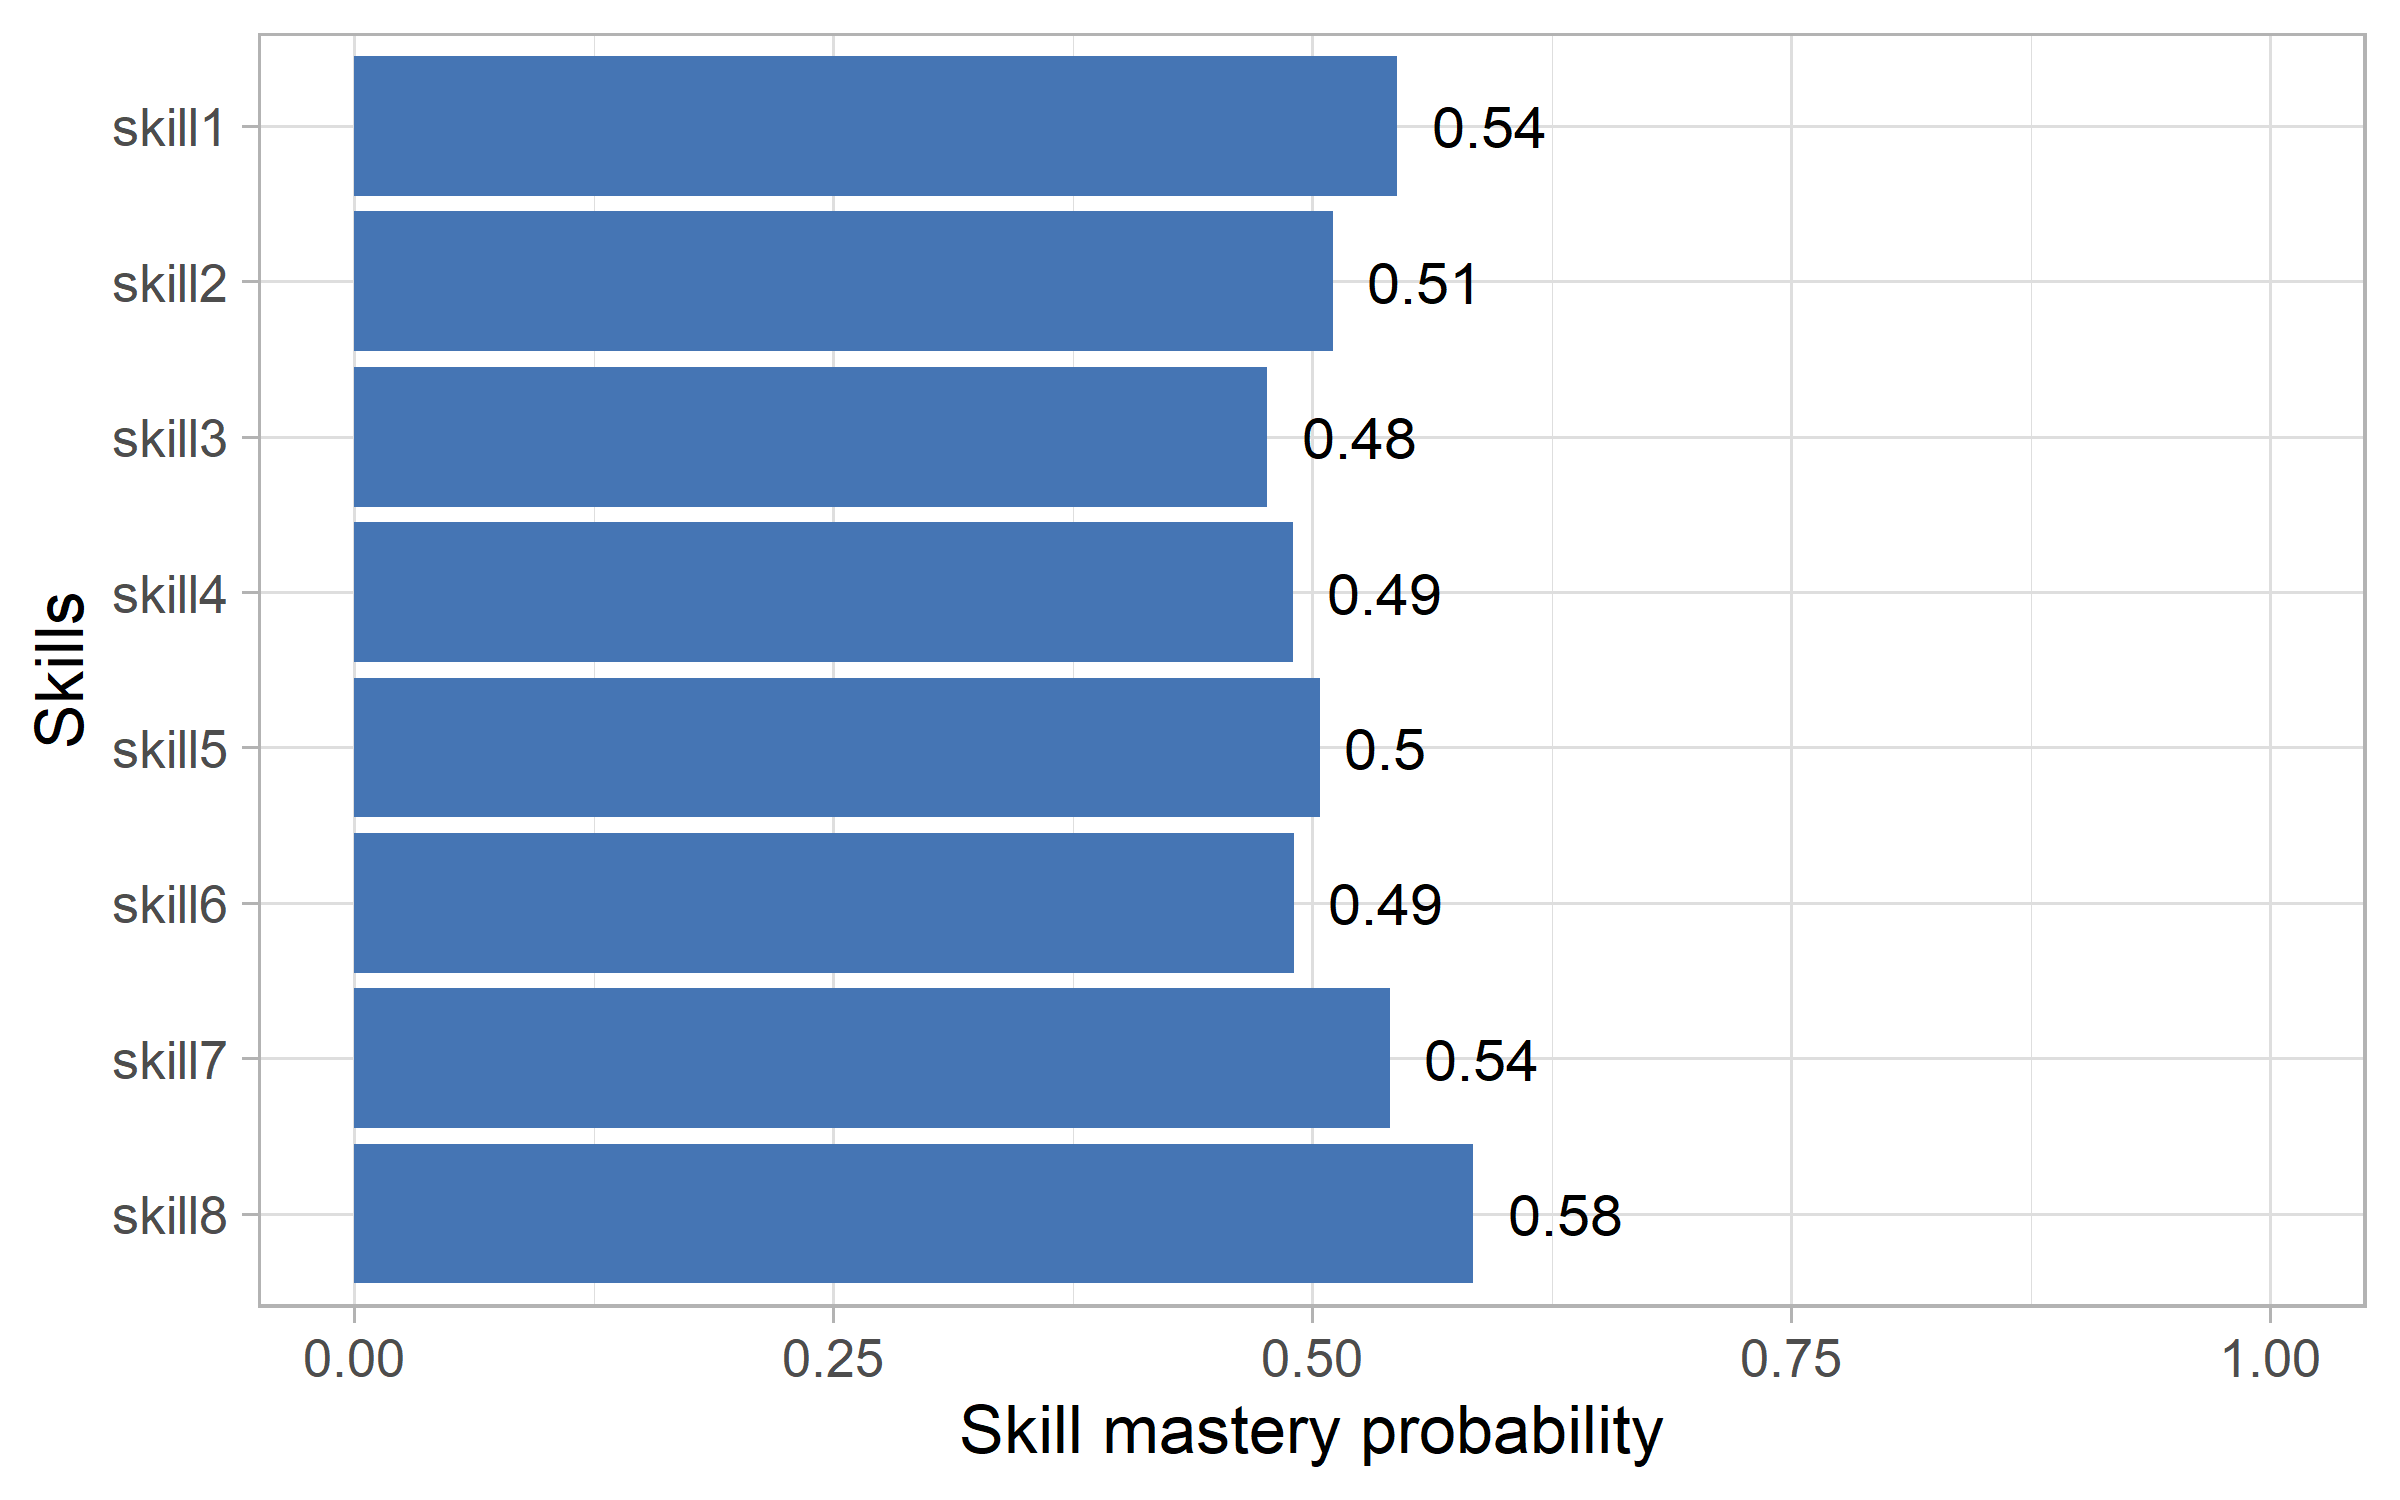
\includegraphics[width=0.7\textwidth]{Skill_mastery_probability_sim.png}
		\caption{Plot of the skill distribution $P(\alpha_k)$.}
		\label{skill_possession_sim}
	\end{figure}
	
	Comparing the results for real data with the results for simulated data leads to conclusions such as that the test group must have had a very good knowledge of subtracting fractions because the obtained results are very positive. It also raises important questions, such as whether the test was created in the best possible way and whether there is a~solution that would improve the simulation results since the simulation results differed so significantly from the results on the group of students. To try to answer those questions, it can be simulated subtracting or adding $Q$-matrix vectors and checking the results.
	
	The first simulation was to reduce the size of the $Q$-matrix. In each iteration, one of the randomly selected rows of the $Q$-matrix was removed from it, then the simulation was performed in the same way as before. The informedness measure and the average skill mastery probability value were used to check the results. For each size of the $Q$-matrix, the simulation was repeated 100 times to get more accurate results. 
	
	Figure \ref{smaller_qmat} shows the values of the obtained parameters. More interesting are results obtained for the informedness measure, because a downward trend is noticeable what allows stating that reducing the number of $q$-vectors adversely affects informedness. The~plot showing the average value of skill mastery probability does not allow drawing clear conclusions, but there is a noticeable jump on the plot, when the percentage of vectors removed from the $Q$-matrix is equal to 65\%. The mean skill mastery probability for 7 from 20 $q$-vectors is around 0.55.
	
	\begin{figure}[h!]
		\centering
		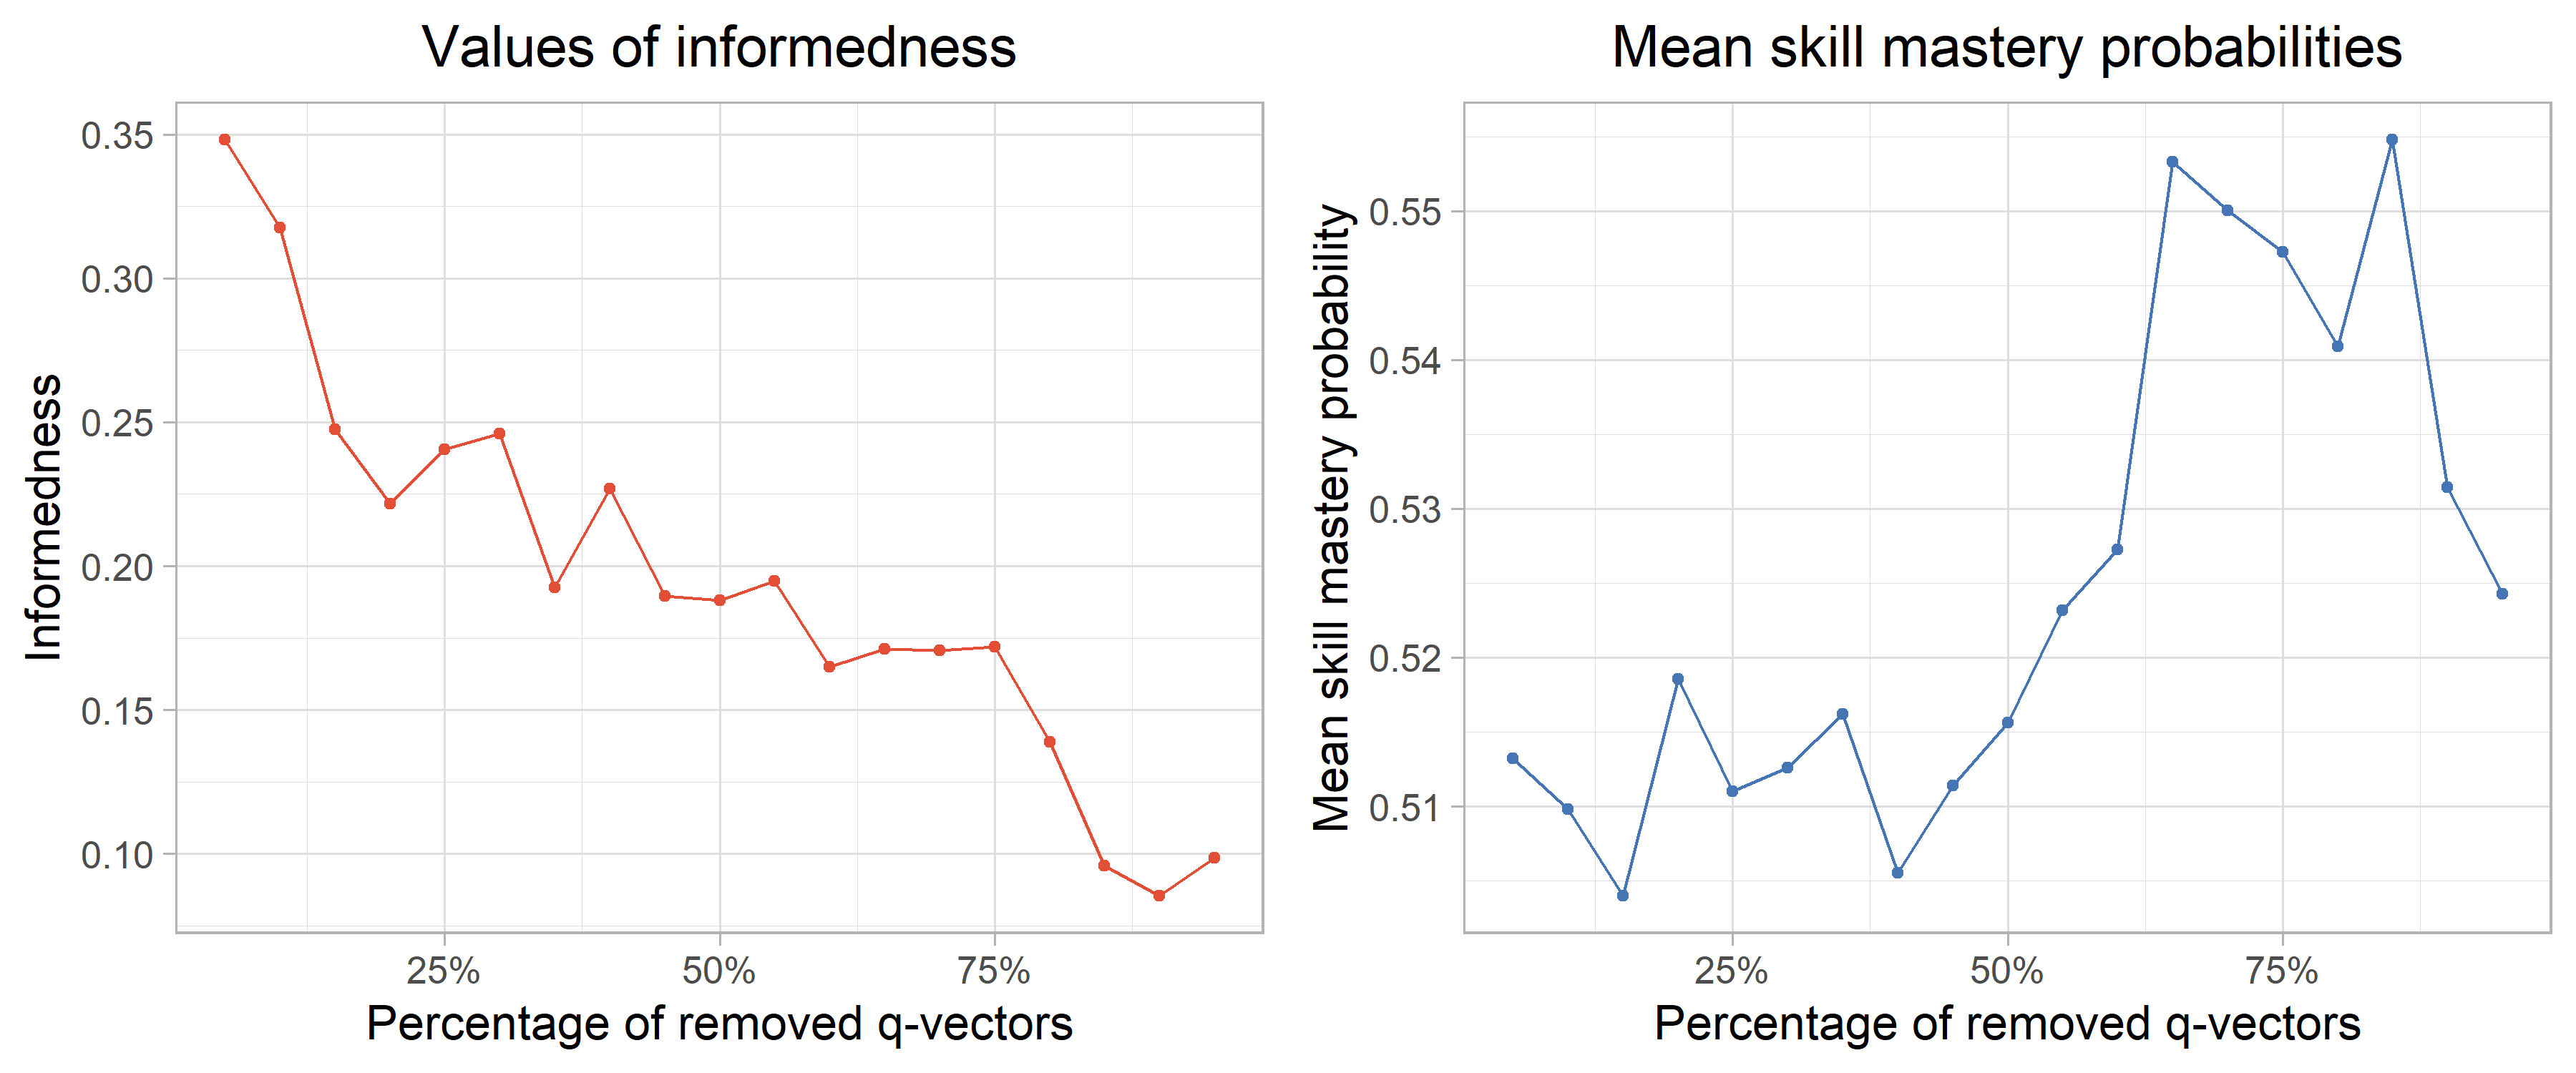
\includegraphics[width=\textwidth]{Smaller_qmatrix_results2.png}
		\caption{Values of the parameters obtained for $Q$-matrix with removed $q$-vectors.}
		\label{smaller_qmat}
	\end{figure}
	
	The second simulation was to increase the size of the $Q$-matrix. In each iteration, one of the randomly selected rows of the $Q$-matrix was added to it. The simulation and analysis were performed in the same way as before and repeated 100 times again. 
	
	Figure \ref{bigger_qmat} shows the values of the obtained parameters. This time the results are not as obvious as before. It can be concluded that the informedness value hovers around the value for the original $Q$-matrix. There is a noticeable jump on the plot of mean skill mastery probabilities, when the percentage of vectors added to the $Q$-matrix is equal to 65\%, which means adding 13 additional $q$-vectors. The mean value drops below 0.50 then. It~should be considered whether extending the test will not affect the concentration of the examinees and whether the improvement of the informedness value is significant enough to make it meaningful.
	
	\begin{figure}[H]
		\centering
		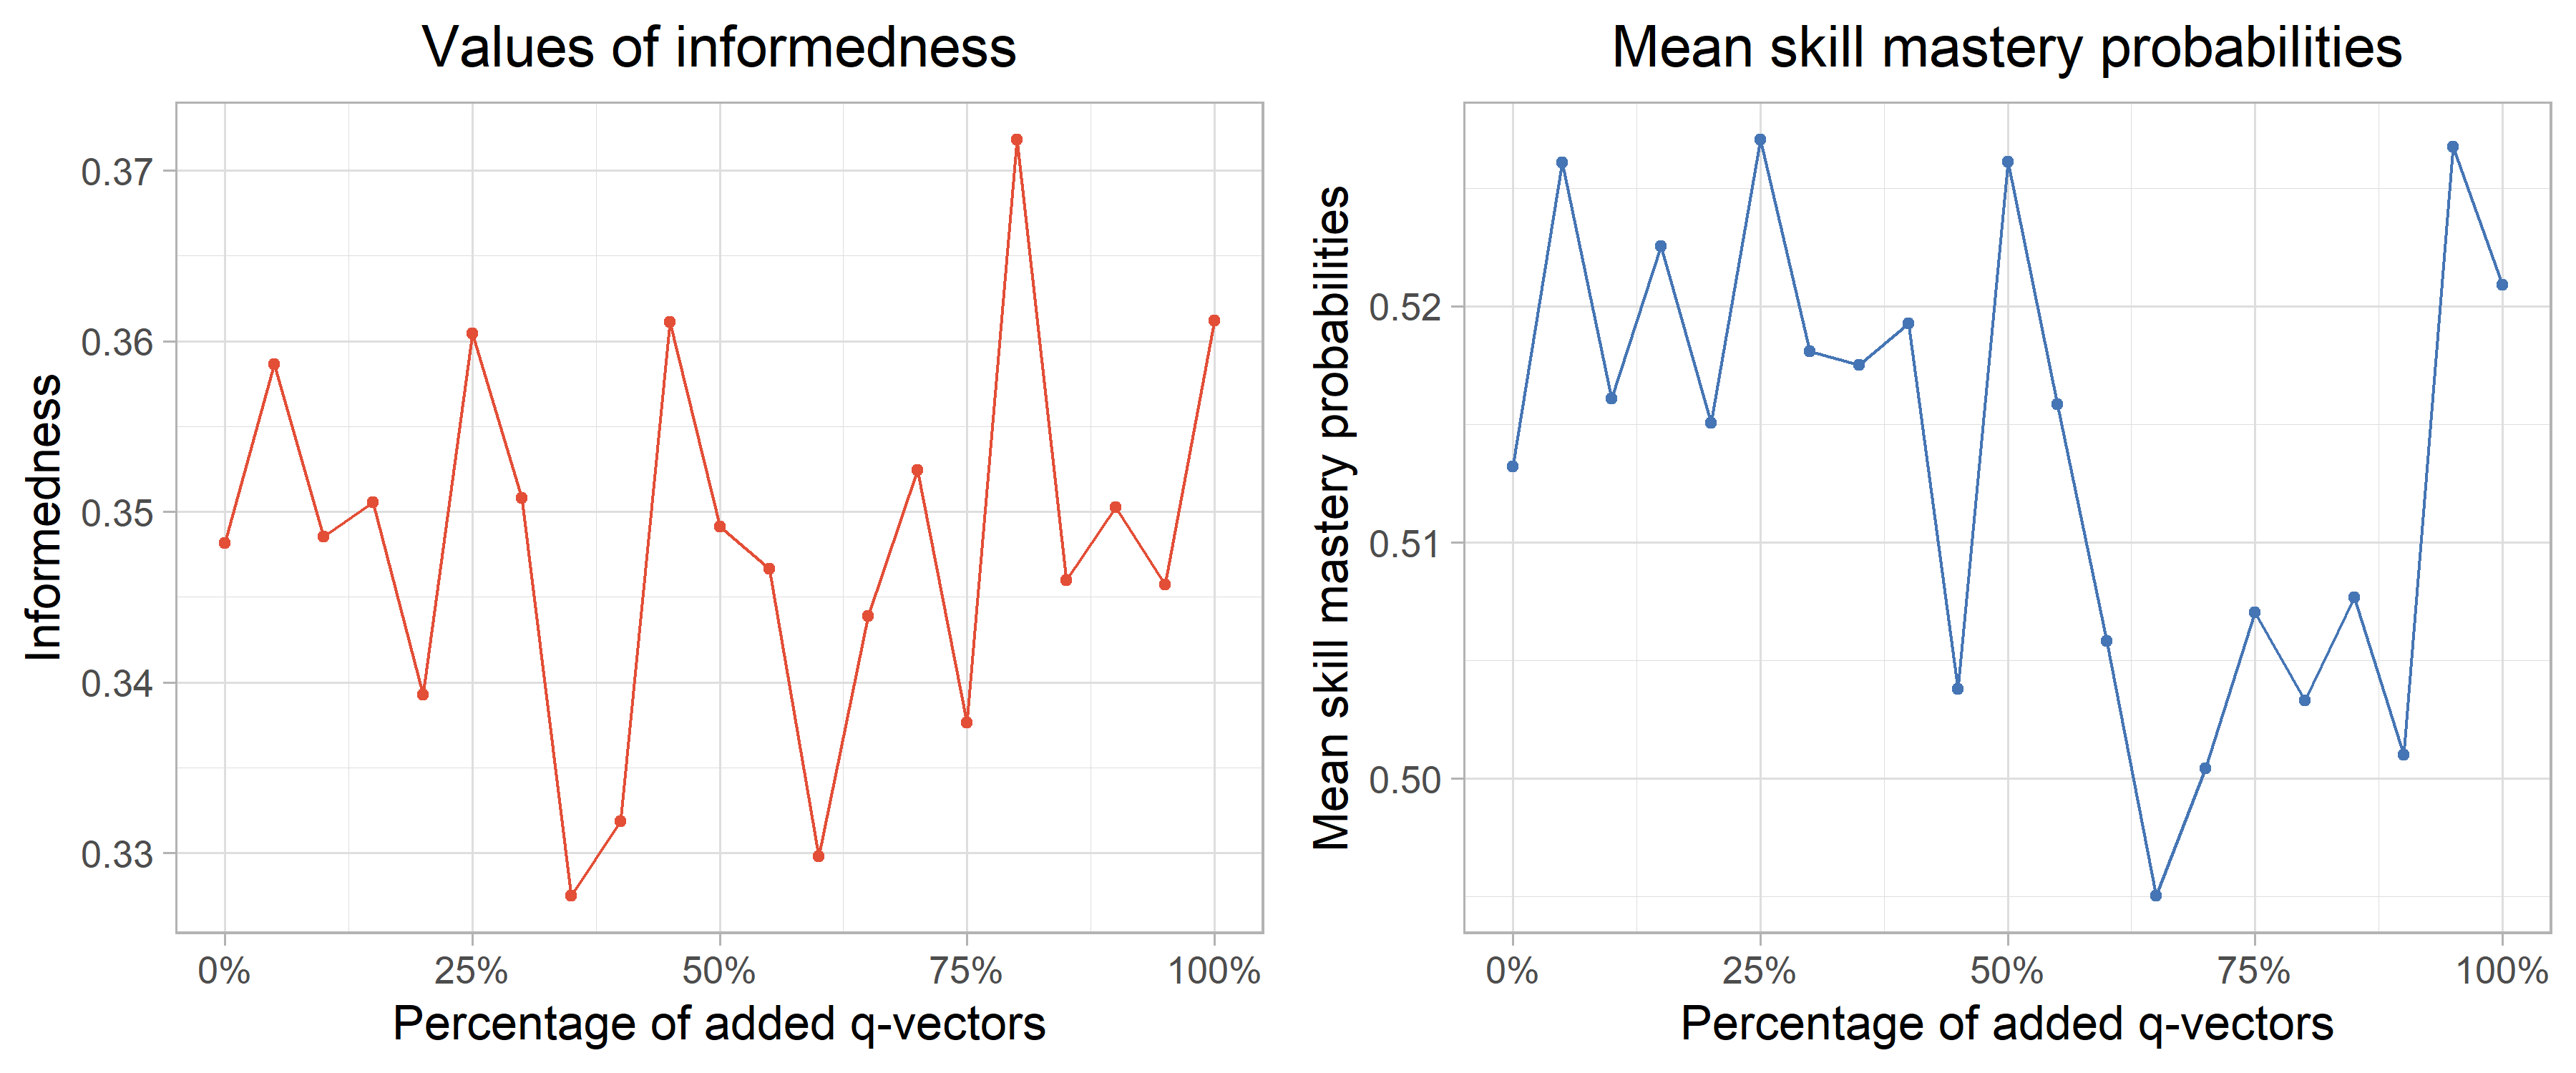
\includegraphics[width=\textwidth]{Bigger_qmatrix_results2.png}
		\caption{Values of the parameters obtained for $Q$-matrix with added $q$-vectors.}
		\label{bigger_qmat}
	\end{figure}
	
	To sum up, the 8-skill test is not the simplest one. It is hard to find a balance between the number of skills tested and the number of items. However, after analyzing the obtained results, it can be concluded that the test chosen to analyze fraction subtraction skills is doing well enough and the created $Q$-matrix is correct.
	
	{\backmatter \chapter{Summary and discussion}}
	
	%W podsumowaniu napisać o tym, że ta praca to zaledwie muśnięcie tematu i że jest w niej pokazane kilka aspektów CDMs - i sprawdzanie poprawności macierzy i operacje na prawdziwych danych, więc możliwości na rozszerzenie tematu jest super dużo.
	
	The aim of the thesis was a comparison of Cognitive Diagnosis Models and measurment of their robustness to the use of an incorrect model, checking the impact of using an~incorrect $Q$-matrix on the estimation results, and showing the possibilities of Cognitive Diagnosis Models based on the analysis of real data.
	
	The thesis began with explaining what Cognitive Diagnosis Models are, what they can be used for and what are the elements necessary for their analysis. Then, four models with guessing and slipping parameters were described -- DINA, NIDA and G-NIDA models from the group of non-compensatory models and DINO from the group of compensatory models. Later, the Joint Maximum Likelihood Estimation method and the measures and statistics used to check the quality of the estimation were described. The next part was devoted to simulations.
	% Celem pracy było porównanie używanych CDM modeli i sprawdzenie ich odporności na wprowadzenie błędnego modelu, sprawdzenie wpływu wprowadzenia błędnej Q-macierzy na wyniki estymacji, a także pokazanie możliwości modeli CDM na podstawie analizy danych rzeczywistych. Praca rozpoczęła się od wyjaśnienia, czym są modele CDM, do czego mogą zostać wykorzystane oraz jakie są elementy niezbędne do przeprowadzenia ich analizy. Następnie opisane zostały cztery modele, które charakteryzowały się parametrami zgadywania i poślizgnięcia -- DINA, NIDA i G-NIDA models z grupy modeli niekompensacyjnych oraz DINO z grupy modeli kompensacyjnych. Pózniej została opisana metoda estymacji tych modeli -- Joint Maximum Likelihood Estimation method oraz miary i statystyki wykorzystane do sprawdzenia jakości estymacji. Kolejna część została poświęcona symulacjom. 
	
	First, an analysis of the CDM misspecification was carried out using the previously described models. On the basis of the obtained results, it was found that the most optimal model, which is simple and the least sensitive to incorrect use of one of the other three models, is the DINA model. Moreover, it was noticed that if the NIDA model is a misspecified model when the true model is DINO, the estimation results are almost random. This result allowed to conclude that if the problem can be solved in several ways and there are indications that the true model is a compensatory model, then the NIDA model should not be chosen for estimation.
	% Najpierw została przeprowadzona analiza błędnej specyfikacji modelu z wykorzystaniem opisanych wcześniej modeli. Na podstawie otrzymanych wyników ustalono, że najbardziej optymalnym modelem, który jest prosty i najmniej wrażliwy na błędne wprowadzenie jednego z trzech pozostałych modeli, jest model DINA. Ponadto, zauważono, że w przypadku wprowadzenia błędnie modelu NIDA, gdy oryginalnym modelem jest DINO, wyniki estymacji są niemalże losowe, co pozwoliło na wyciągnięcie wniosku, że jeżeli zadanie może być rozwiązane na kilka sposobów i są przesłanki, że oryginalnym modelem jest model kompensacyjny, to do estymacji nie powinno się wybierać modelu NIDA.
	
	The next part of the simulation concerned the examination of the impact of the $Q$-matrix misspecification. Several types of misspecification have been investigated. It was noticed that for over- and underspecification, better results were obtained for underspecification. This is an important conclusion for experts who create the $Q$-matrix and they have doubts about the requirement of an attribute for giving a positive response -- it is better not to include it in the $Q$-matrix because an underestimated matrix gives better results than overestimated.
	% Kolejna część symulacyjna dotyczyła zbadania wpływu błędnej specyfikacji Q-macierzy. Zostało zbadane kilka rodzajów misspecification. Zauważono, że przypadku over i underspecification, lepsze wyniki otrzymane zostały w przypadku niedoszacowania. Jest to ważny wniosek dla osób, które zajmują się tworzeniem macierzy i wymaganie jakiejś umiejętności budzi ich wątpliwość - lepiej jest nie umieszczać jej w macierzy, ponieważ niedoszacowana macierz daje lepsze rezultaty.  
	
	The last part of the thesis concerned the analysis of the real data. The group of respondents was small, but this did not prevent from drawing interesting conclusions. Most students were found to have the skills necessary to subtract fractions. The most difficult skills for some students were separating a whole number from a fraction and simplifying before substracting. There were no items that turned out to be extremely difficult. Most of the item allowed for the separation of groups of students who could solve them from those who could not. After the analysis of the real data, a simulation was performed on the real $Q$-matrix and with the slipping and guessing parameters estimated on the real data. It was noticed that the simulation results differ significantly from the real ones. The test, in fact, was much more difficult, which confirmed that the tested group had mastered the required skills. The last subject of the analysis was to check whether removing or adding items to the $Q$-matrix would improve the estimation results. It was found that removing items negatively affects the obtained results, while adding items may improve the results, but the improvement is so small that it is not worth the additional involvement of students and teachers.
	% Ostatnia część pracy dotyczyła analizy danych rzeczywistych. Grupa badanych była dość mała, jednak nie przeszkodziło to w wyciągnięciu interesujących wniosków. Stwierdzono, że większość uczniów posiadała umiejętności niezbędne do odejmowania ułamków. Umiejętności, które sprawiały najwięcej trudności części uczniów, to 2,3. Nie było zadań, które okazały się być wyjątkowo trudne. Większość z zadań pozwalała na oddziele grupy uczniów potrafiących je rozwiązać od tych, którzy nie potrafili. Po przeprowadzonej analizie dokonano symulacji na rzeczywistej Q-macierzy i z wyestymowanymi na rzeczywistych danych parametrami s i g. Zauważono, że wyniki symulacyjne znacznie różnią się od tych rzeczywistych. Test w swej istotnie był zdecydowanie trudniejszy, co potwierdziło, że badana grupa opanowała umiejętności. Ostatnim przedmiotem analizy było sprawdzenie, czy usunięcie lub dodanie zadań do macierzy wpłynie na poprawę wyników estymacji. Stwierdzono, że usunięcie zadań wpływa negatywnie na otrzymane wyniki, natomiast dodanie może poprawić wyniki, ale poprawa jest na tyle niewielka, że nie jest to warte dodatkowego zaangażowania uczniów i nauczycieli.
	
	Based on the simulations and analyzes, it can be concluded that Cognitive Diagnosis Models are an interesting tool that can give researchers and teachers many possibilities. It~is a tool that, when used in education, could significantly contribute to the improvement of the quality of teaching, as it is able to provide detailed information on the strengths and weaknesses of the tested students. The above thesis is only an introduction to Cognitive Diagnosis Models as it is a very broad topic offering many possibilities. The conducted research could be enriched with further Cognitive Diagnosis Models, which can also be subject to sensitivity analysis to model misspecification. Possible development of the work could also be the analysis of other types of incorrectly specified $Q$-matrices.
	% Na podstawie przeprowadzonych symulacji i analiz można stwierdzić, że Cognitive Diagnosis Models są ciekawym narzędziem, które może dać wiele możliwości. Jest to narzędzie, które wykorzystywane w edukacji, mogłoby znacząco przyczynić się do poprawy jakości nauczania, ponieważ jest w stanie dostarczyć szczegółowych informacji na temat mocnych i słabych stron sprawdzanych uczniów. Powyższa praca jest zaledwie wprowadzeniem do CDMs, ponieważ jest to bardzo obszerny temat, który daje wiele możliwości. Przeprowadzone badania mogłyby zostać wzbogacone o kolejne modele kognitywistyczne, które także można poddać analizie wrażliwości na błędną specyfikację modelu. Możliwym rozwinięciem pracy mogłaby być także analiza innych rodzajów błędnie sprecyzowanej Q-macierzy.
	
	
	\appendix
	{\chapter{Functions}}\label{appendix}
	
	\noindent The appendix lists the functions that were used to run the simulations -- generating a~random $Q$-matrix, random skill profiles and, as a~result, a response matrix. \vspace{5pt}
	
	
	\begin{itemize}
		
		\item  Function \texttt{SolveTest()} is a solution of the test, what means it returns the response data -- binary matrix with value 1 if examinee solved the item correctly or 0 if not. The possible Cognitive Diagnosis Models are DINA, DINO, NIDA and G-NIDA.
		
		\lstinputlisting[language=R, linerange={11-55}]{CDMfunctions.R}
		
		\item Function \texttt{SkillProfiles()} randomly choose a sample of skills of chosen number of examinees from all possible combinations named \texttt{SkillsClass}.
		
		\lstinputlisting[language=R, linerange={66-70}]{CDMfunctions.R}
		
		\noindent where, for number K equal to number of skills, variable \texttt{SkillsClass} is defined as
		
		\lstinputlisting[language=R, linerange={76-76}]{CDMfunctions.R}
		
		\item Function \texttt{ChooseQmatrix()} randomly choose $Q$-matrix from all possible combinations of skills needed. 
		
		\lstinputlisting[language=R, linerange={81-88}]{CDMfunctions.R}
		
	\end{itemize}
	
	% Dodatek w pracach matematycznych również nie jest wymagany. Można w nim przedstawić np. jakiś dłuższy dowód, który z pewnych przyczyn pominęliśmy we właściwej części pracy lub (np. w przypadku prac statystycznych) umieścić dane, które analizowaliśmy.
	
	
	
	%%%%%%%%%%%%%%%%%%%%%%%%%%%%%%%%%%%%%%%%%%%%%%%%%%%%%%%%%
	% BIBLIOGRAFIA
	% W tworzeniu bibliografii najlepiej korzystać z BibTex'a, 
	% który jest częścią systemu Tex. W naszym przypadku funkcję 
	% przechowalni literatury, do której się odwołujemy, pełni 
	% plik bibliografia.bib. Nie musimy ręcznie dodawać nowych 
	% pozycji do bibliografii. Możemy wejść np. na stronę 
	% https://mathscinet.ams.org/mathscinet/index.html, 
	% znaleźć odpowiednią pozycję, wybrać ją, a następnie zmienić 
	% 'Select alternative format' na BibTeX, skopiować uzyskany 
	% tekst, wkleić do pliku bibliografia.bib i skompilować. 
	% Gotowe informacje do pliku bibliografia.bib można znaleźć 
	% także na https://arxiv.org - gdy znajdziemy interesującą nas 
	% pracę, szukamy 'References & Citations' i klikamy 'NASA ADS', 
	% a potem 'Bibtex entry for this abstract' 
	% i postępujemy tak jak wcześniej.
	%%%%%%%%%%%%%%%%%%%%%%%%%%%%%%%%%%%%%%%%%%%%%%%%%%%%%%%%%
	\newpage
	\bibliografia{bibliografia} 
	
	%https://www.ncbi.nlm.nih.gov/pmc/articles/PMC6092632/
\end{document}